\documentclass[]{elsarticle} %review=doublespace preprint=single 5p=2 column
%%% Begin My package additions %%%%%%%%%%%%%%%%%%%

\usepackage[hyphens]{url}


\usepackage{graphicx}
%%%%%%%%%%%%%%%% end my additions to header

\usepackage[T1]{fontenc}
\usepackage{lmodern}
\usepackage{amssymb,amsmath}
% TODO: Currently lineno needs to be loaded after amsmath because of conflict
% https://github.com/latex-lineno/lineno/issues/5
\usepackage{lineno} % add
\usepackage{ifxetex,ifluatex}
\usepackage{fixltx2e} % provides \textsubscript
% use upquote if available, for straight quotes in verbatim environments
\IfFileExists{upquote.sty}{\usepackage{upquote}}{}
\ifnum 0\ifxetex 1\fi\ifluatex 1\fi=0 % if pdftex
  \usepackage[utf8]{inputenc}
\else % if luatex or xelatex
  \usepackage{fontspec}
  \ifxetex
    \usepackage{xltxtra,xunicode}
  \fi
  \defaultfontfeatures{Mapping=tex-text,Scale=MatchLowercase}
  \newcommand{\euro}{€}
\fi
% use microtype if available
\IfFileExists{microtype.sty}{\usepackage{microtype}}{}
\usepackage[]{natbib}
\bibliographystyle{plainnat}

\ifxetex
  \usepackage[setpagesize=false, % page size defined by xetex
              unicode=false, % unicode breaks when used with xetex
              xetex]{hyperref}
\else
  \usepackage[unicode=true]{hyperref}
\fi
\hypersetup{breaklinks=true,
            bookmarks=true,
            pdfauthor={Márton Kiss},
            pdftitle={Cookbook},
            colorlinks=false,
            urlcolor=blue,
            linkcolor=magenta,
            pdfborder={0 0 0}}

\setcounter{secnumdepth}{0}
% Pandoc toggle for numbering sections (defaults to be off)
\setcounter{secnumdepth}{0}

% Pandoc syntax highlighting
\usepackage{color}
\usepackage{fancyvrb}
\newcommand{\VerbBar}{|}
\newcommand{\VERB}{\Verb[commandchars=\\\{\}]}
\DefineVerbatimEnvironment{Highlighting}{Verbatim}{commandchars=\\\{\}}
% Add ',fontsize=\small' for more characters per line
\usepackage{framed}
\definecolor{shadecolor}{RGB}{248,248,248}
\newenvironment{Shaded}{\begin{snugshade}}{\end{snugshade}}
\newcommand{\AlertTok}[1]{\textcolor[rgb]{0.94,0.16,0.16}{#1}}
\newcommand{\AnnotationTok}[1]{\textcolor[rgb]{0.56,0.35,0.01}{\textbf{\textit{#1}}}}
\newcommand{\AttributeTok}[1]{\textcolor[rgb]{0.77,0.63,0.00}{#1}}
\newcommand{\BaseNTok}[1]{\textcolor[rgb]{0.00,0.00,0.81}{#1}}
\newcommand{\BuiltInTok}[1]{#1}
\newcommand{\CharTok}[1]{\textcolor[rgb]{0.31,0.60,0.02}{#1}}
\newcommand{\CommentTok}[1]{\textcolor[rgb]{0.56,0.35,0.01}{\textit{#1}}}
\newcommand{\CommentVarTok}[1]{\textcolor[rgb]{0.56,0.35,0.01}{\textbf{\textit{#1}}}}
\newcommand{\ConstantTok}[1]{\textcolor[rgb]{0.00,0.00,0.00}{#1}}
\newcommand{\ControlFlowTok}[1]{\textcolor[rgb]{0.13,0.29,0.53}{\textbf{#1}}}
\newcommand{\DataTypeTok}[1]{\textcolor[rgb]{0.13,0.29,0.53}{#1}}
\newcommand{\DecValTok}[1]{\textcolor[rgb]{0.00,0.00,0.81}{#1}}
\newcommand{\DocumentationTok}[1]{\textcolor[rgb]{0.56,0.35,0.01}{\textbf{\textit{#1}}}}
\newcommand{\ErrorTok}[1]{\textcolor[rgb]{0.64,0.00,0.00}{\textbf{#1}}}
\newcommand{\ExtensionTok}[1]{#1}
\newcommand{\FloatTok}[1]{\textcolor[rgb]{0.00,0.00,0.81}{#1}}
\newcommand{\FunctionTok}[1]{\textcolor[rgb]{0.00,0.00,0.00}{#1}}
\newcommand{\ImportTok}[1]{#1}
\newcommand{\InformationTok}[1]{\textcolor[rgb]{0.56,0.35,0.01}{\textbf{\textit{#1}}}}
\newcommand{\KeywordTok}[1]{\textcolor[rgb]{0.13,0.29,0.53}{\textbf{#1}}}
\newcommand{\NormalTok}[1]{#1}
\newcommand{\OperatorTok}[1]{\textcolor[rgb]{0.81,0.36,0.00}{\textbf{#1}}}
\newcommand{\OtherTok}[1]{\textcolor[rgb]{0.56,0.35,0.01}{#1}}
\newcommand{\PreprocessorTok}[1]{\textcolor[rgb]{0.56,0.35,0.01}{\textit{#1}}}
\newcommand{\RegionMarkerTok}[1]{#1}
\newcommand{\SpecialCharTok}[1]{\textcolor[rgb]{0.00,0.00,0.00}{#1}}
\newcommand{\SpecialStringTok}[1]{\textcolor[rgb]{0.31,0.60,0.02}{#1}}
\newcommand{\StringTok}[1]{\textcolor[rgb]{0.31,0.60,0.02}{#1}}
\newcommand{\VariableTok}[1]{\textcolor[rgb]{0.00,0.00,0.00}{#1}}
\newcommand{\VerbatimStringTok}[1]{\textcolor[rgb]{0.31,0.60,0.02}{#1}}
\newcommand{\WarningTok}[1]{\textcolor[rgb]{0.56,0.35,0.01}{\textbf{\textit{#1}}}}

% tightlist command for lists without linebreak
\providecommand{\tightlist}{%
  \setlength{\itemsep}{0pt}\setlength{\parskip}{0pt}}




\usepackage{multicol} \usepackage{float} \usepackage{placeins} \usepackage{afterpage} \usepackage{inputenc} \DeclareUnicodeCharacter{0081}{ } \DeclareUnicodeCharacter{03B2}{\ensuremath{\beta}} \DeclareUnicodeCharacter{03C1}{\ensuremath{\rho}} \DeclareUnicodeCharacter{03C3}{\ensuremath{\sigma}} \DeclareUnicodeCharacter{03C4}{\ensuremath{\tau}}
\usepackage{booktabs}
\usepackage{longtable}
\usepackage{array}
\usepackage{multirow}
\usepackage{wrapfig}
\usepackage{float}
\usepackage{colortbl}
\usepackage{pdflscape}
\usepackage{tabu}
\usepackage{threeparttable}
\usepackage{threeparttablex}
\usepackage[normalem]{ulem}
\usepackage{makecell}
\usepackage{xcolor}
\usepackage{caption}
\usepackage{graphicx}
\usepackage{siunitx}
\usepackage{hhline}
\usepackage{calc}
\usepackage{tabularx}
\usepackage{adjustbox}
\usepackage{hyperref}



\begin{document}


\begin{frontmatter}

  \title{Cookbook}
    \author[]{%
  %
  }
  
      \cortext[cor1]{Corresponding author}
  
  \begin{abstract}
  
  \end{abstract}
  
 \end{frontmatter}

\(~\)\\
\(~\)\\
\(~\)\\
\(~\)\\
\(~\)\\
\(~\)\\
\(~\)\\
Date: \_\_\_\_\_\_\_\_\_\_\_\_\_\_\_\_\_\_\_\_\_\_\_ Signature:
\_\_\_\_\_\_\_\_\_\_\_\_\_\_\_\_\_\_\_\_\_\_\_\_\_\_\_\_\_\_\_\_\_\_\_\_
\(~\)\\
\(~\)\\
\(~\)\\
\(~\)\\

\hypertarget{version-control}{%
\subsection*{Version control}\label{version-control}}
\addcontentsline{toc}{subsection}{Version control}

v.1.0 -- Initial version

\newpage

\listoffigures
\listoftables
\pagebreak

\hypertarget{results}{%
\section{Results}\label{results}}

\renewcommand\floatpagefraction{0.8}

\graphicspath{ {../figure} {../inst/cookbook_files/figure-latex/} {../figure-latex/} {../inst/01_chap1_files/figure-latex/}}

\hypertarget{executive-summary}{%
\subsection{Executive summary}\label{executive-summary}}

Lorem ipsum dolor sit amet, consectetur adipiscing elit. Maecenas et
justo non erat lobortis tincidunt. In et nunc sollicitudin, pellentesque
neque sit amet, blandit mauris. Praesent nunc urna, mattis non risus eu,
egestas bibendum nunc. Mauris et hendrerit purus.

Nunc sodales, massa ut vehicula auctor, augue felis faucibus urna, et
semper libero tortor accumsan magna. Proin non tortor quis erat tempor
fermentum et ut tortor. Praesent elementum tristique sapien a interdum.
Aenean sit amet mi a sapien semper ullamcorper. Phasellus quis enim
tempor, porttitor odio eu, faucibus libero. Nullam eu eros vitae eros
dictum luctus. Mauris congue ante vel laoreet eleifend.

\begin{figure}[H]

{\centering 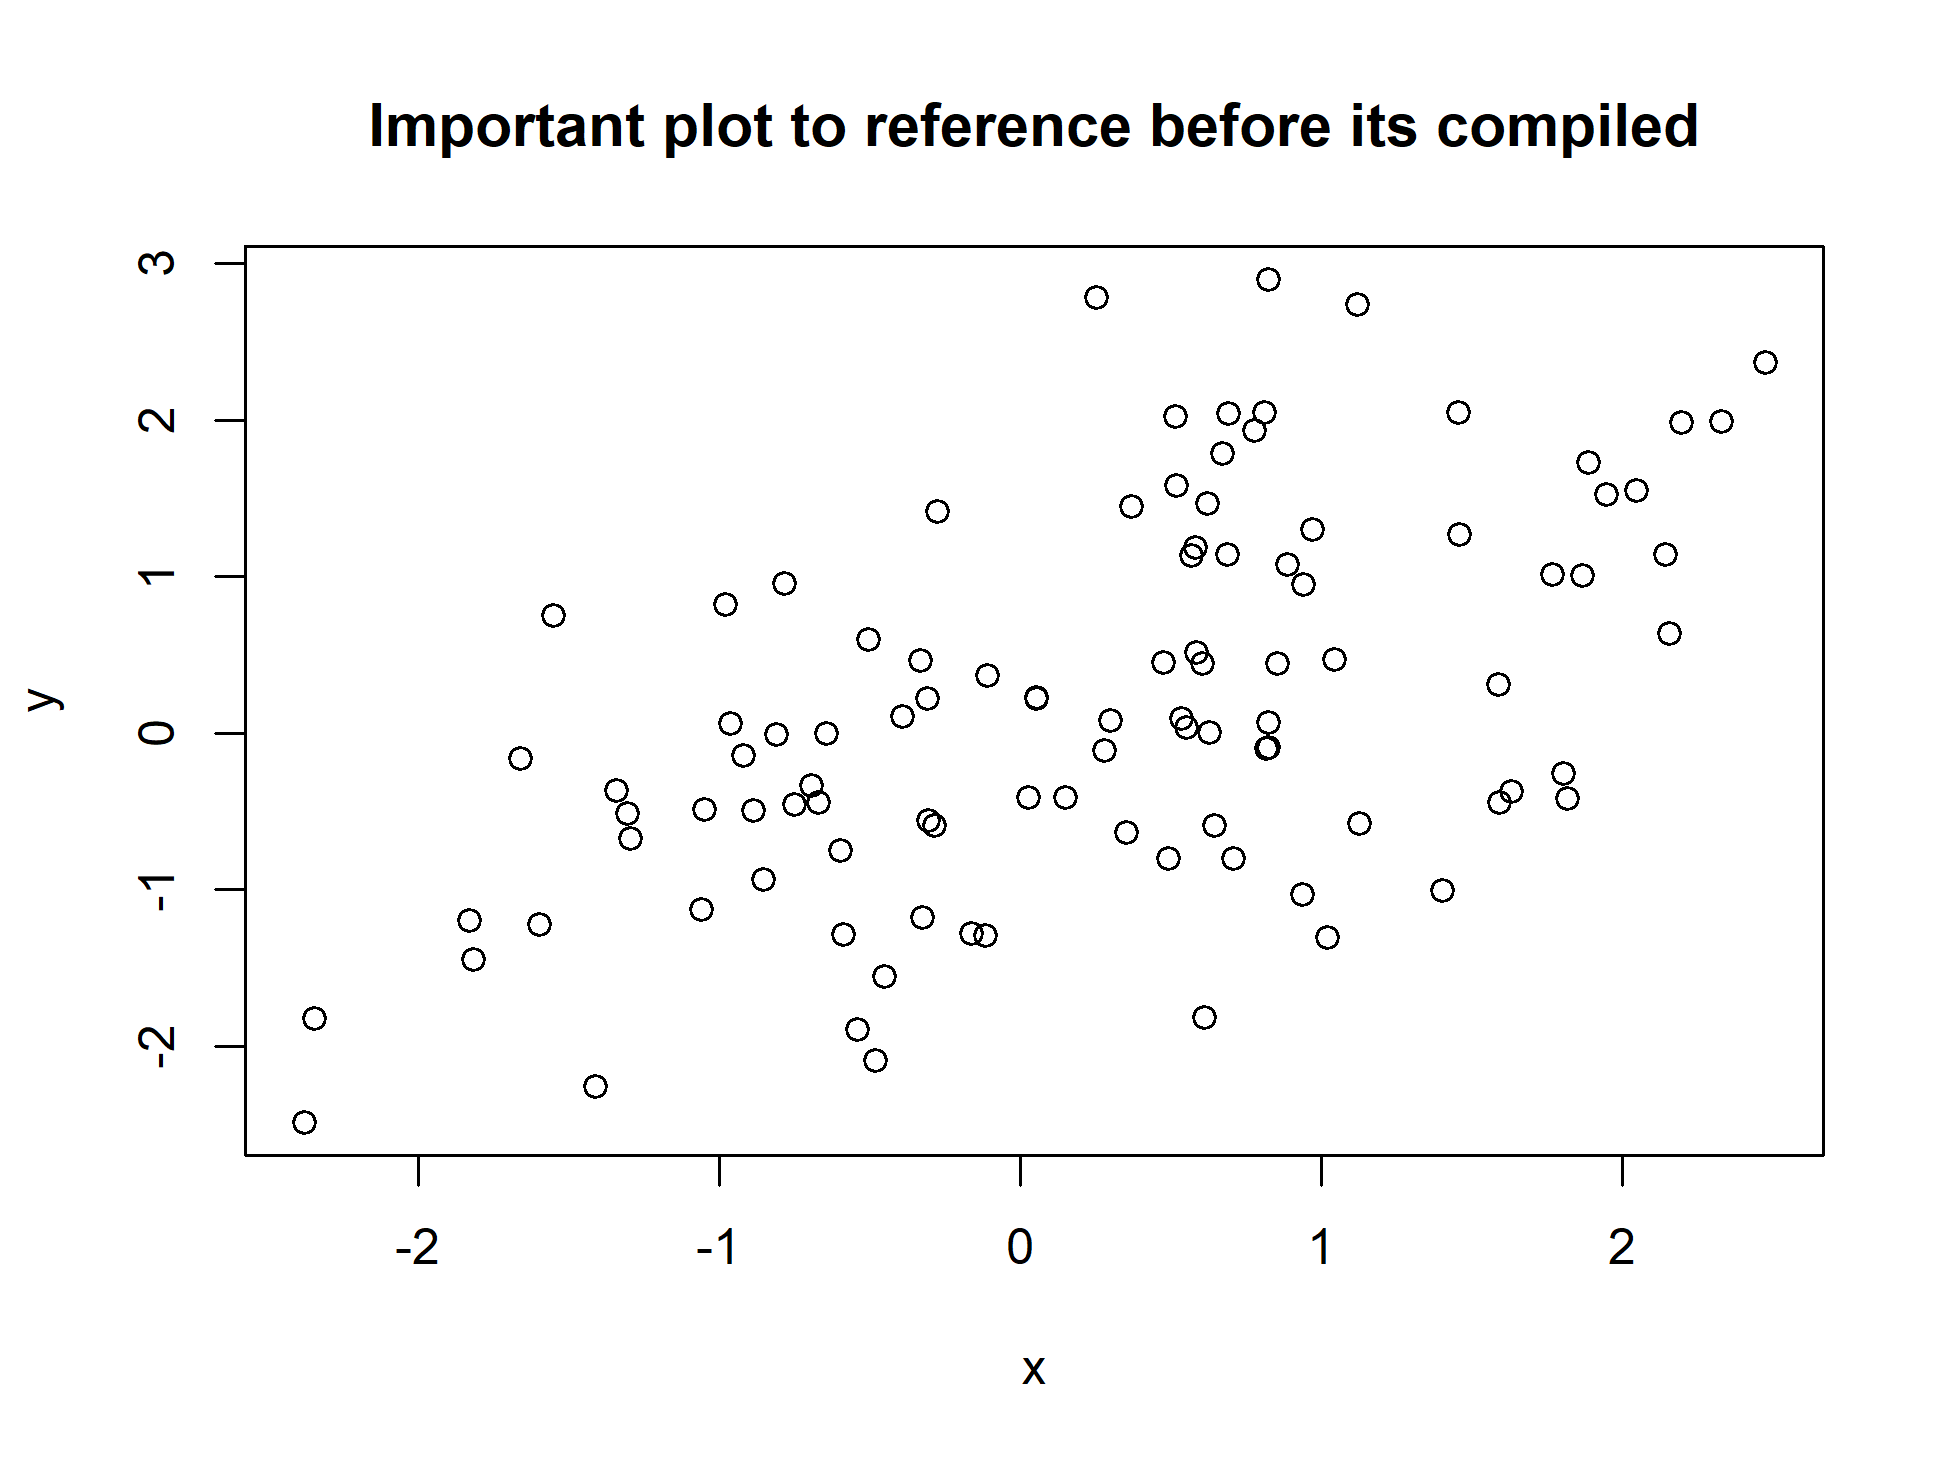
\includegraphics[width=0.9\linewidth]{cookbook_files/figure-latex/chunk-a-1} 

}

\caption{Executive graph for executive thoughts}\label{fig:chunk-a}
\end{figure}

\begin{figure}[H]
\begin{multicols}{2}
\begin{figure}[H]
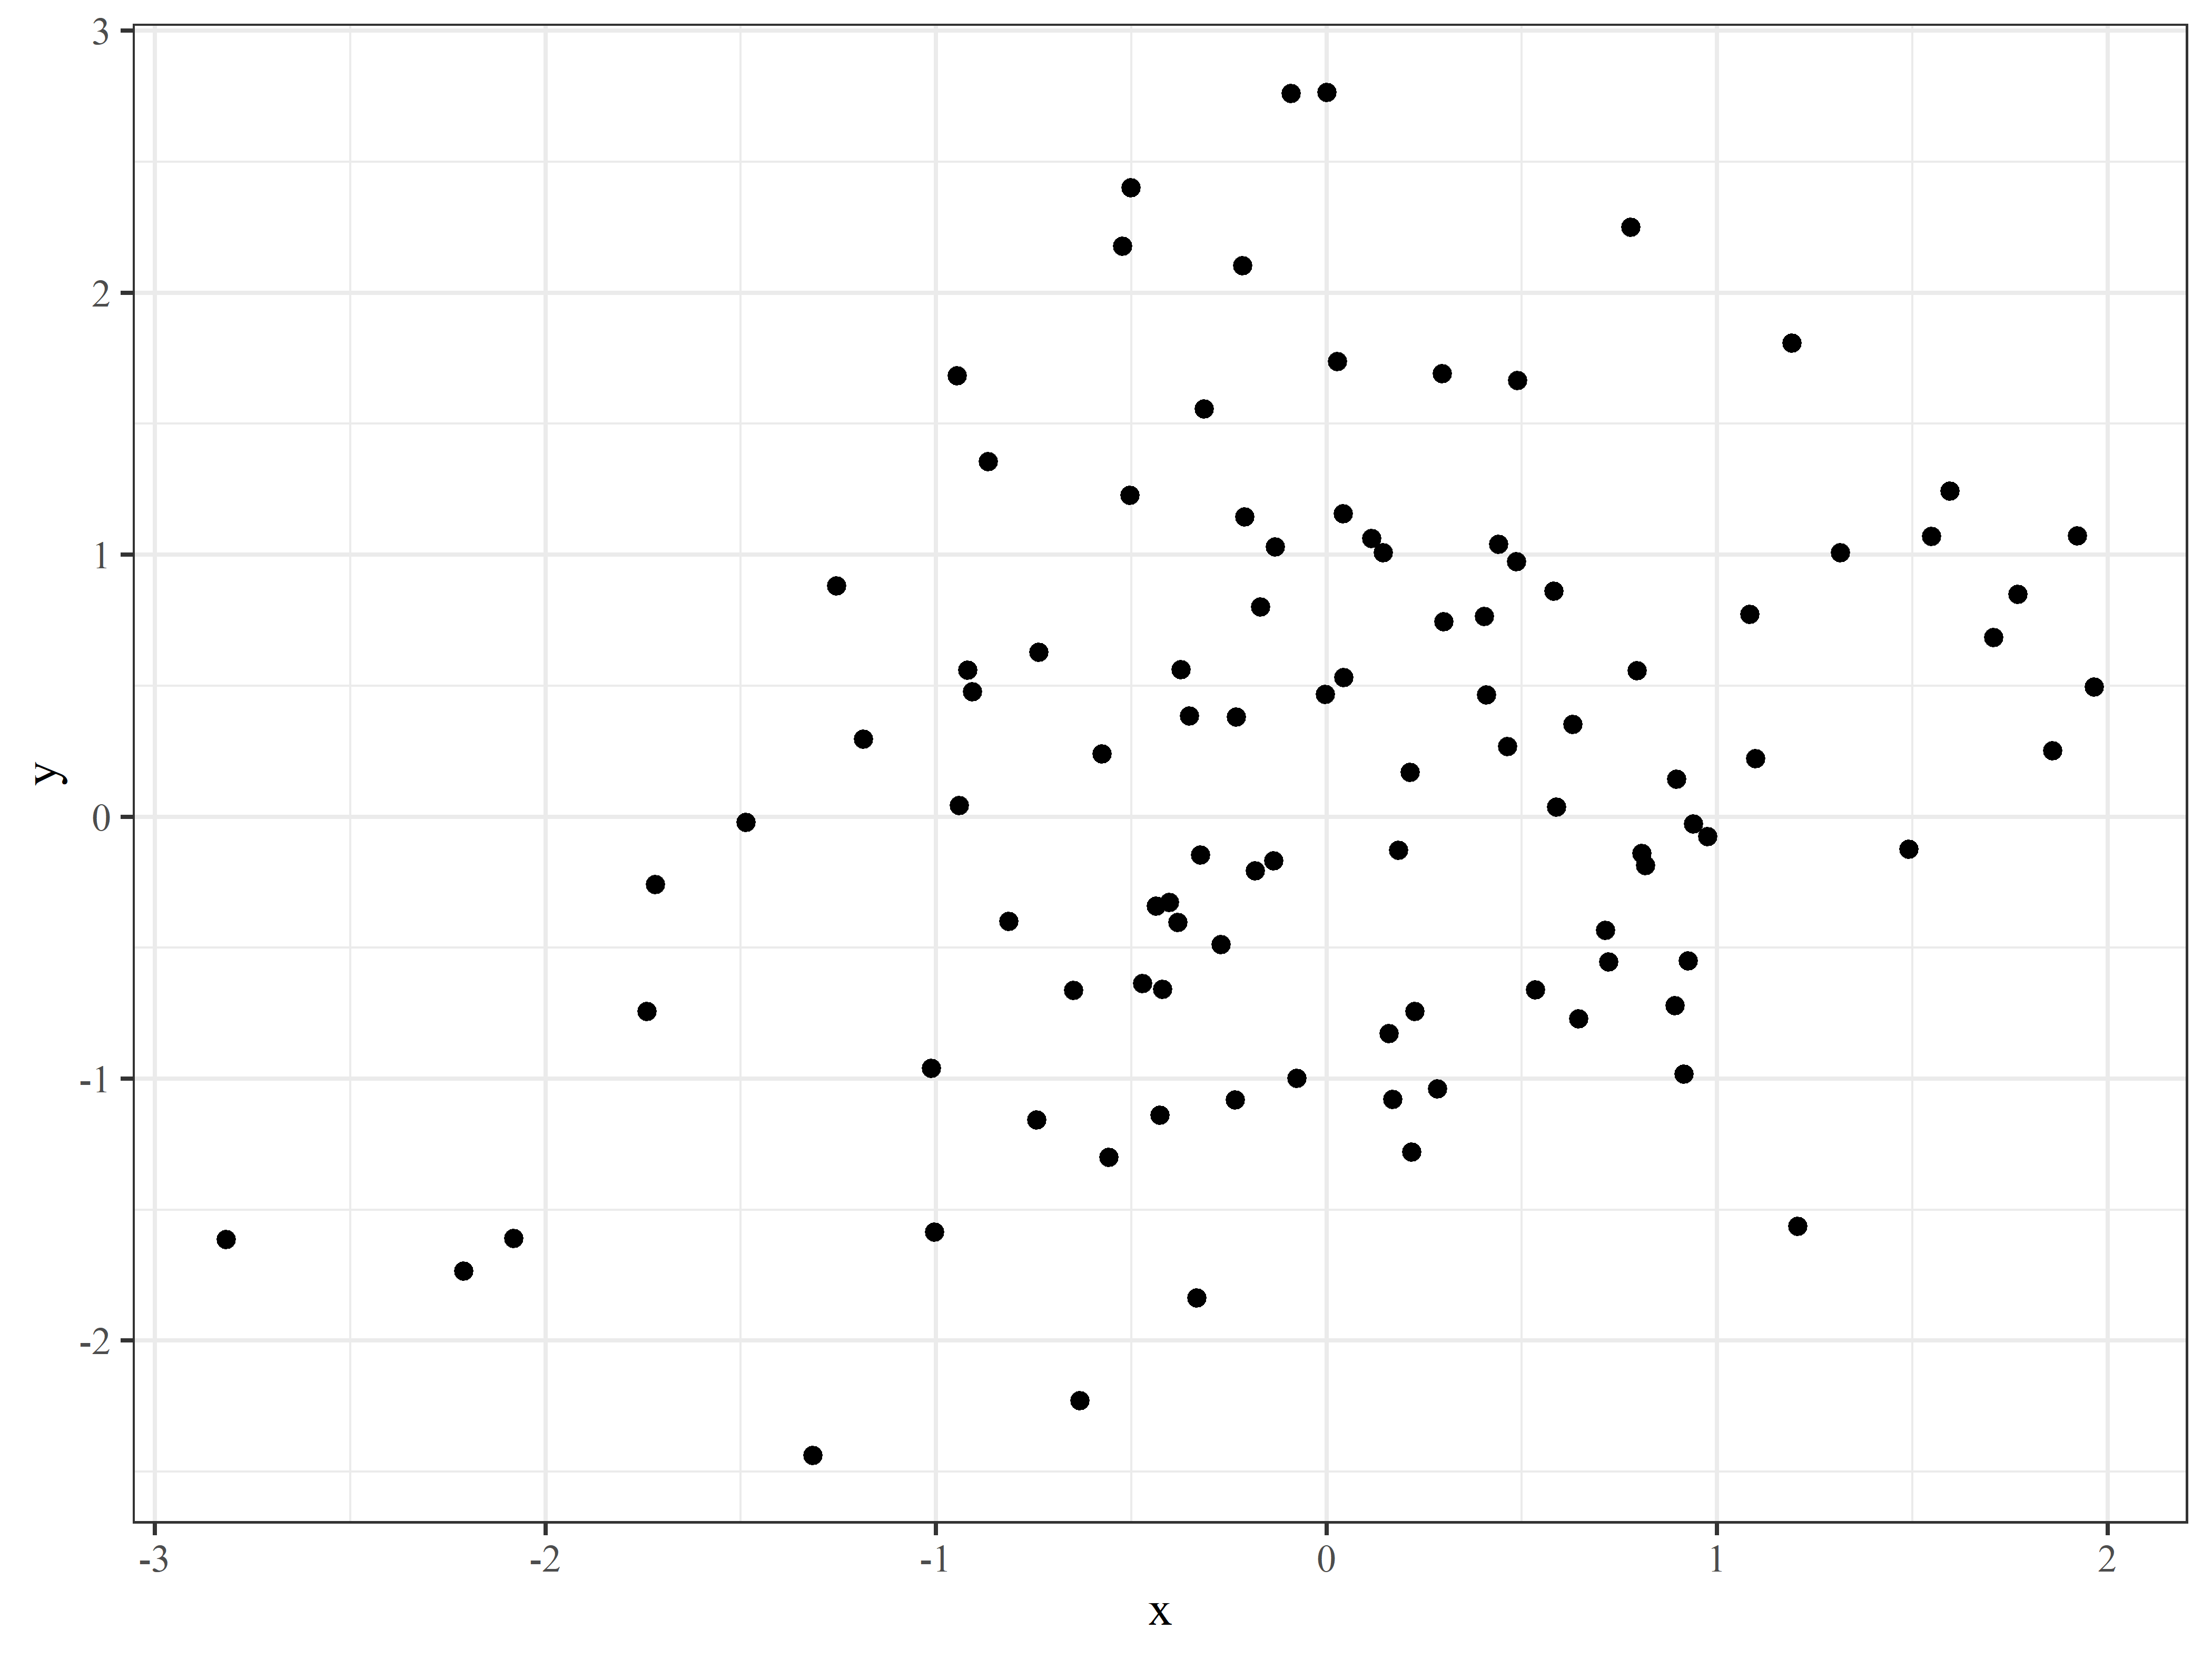
\includegraphics[width = \linewidth]{mandatory_chunk_name-1.png}
\caption{Plot the first}
\label{fig:plotmeans}
\end{figure}

\columnbreak

\begin{figure}[H]
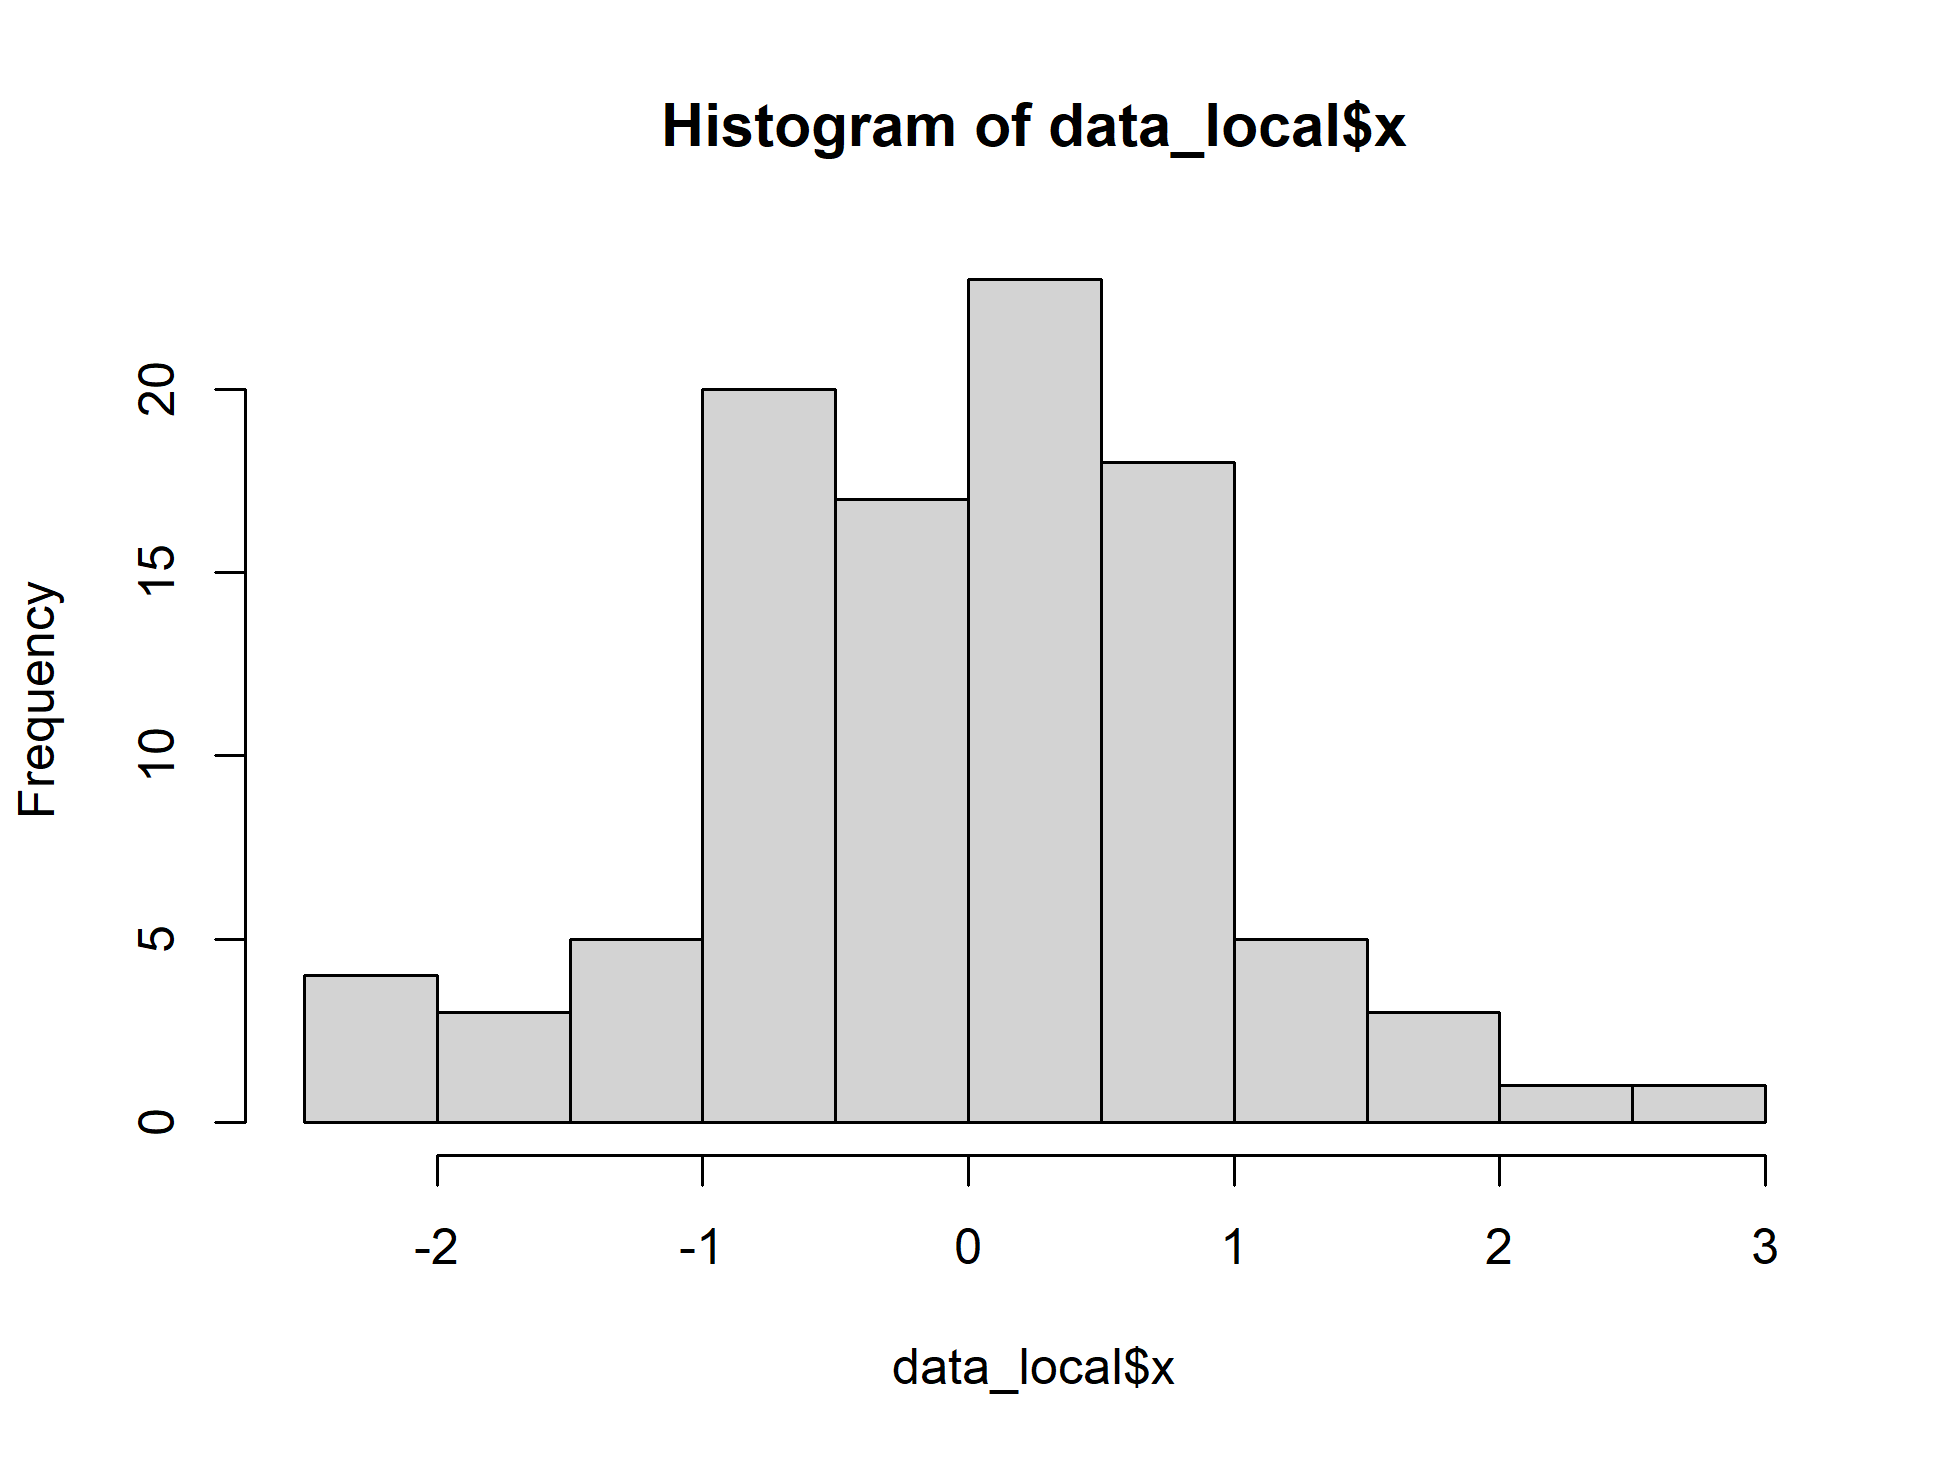
\includegraphics[width = \linewidth]{mandatory_chunk_name-2.png}
\centering
\caption{Plot the second}
\label{fig:histogram}
\end{figure}
\end{multicols}
\end{figure}

\newpage

\hypertarget{introduction}{%
\subsection{Introduction}\label{introduction}}

\begin{verbatim}
This is a text box if you like textboxes
\end{verbatim}

Links can be given in this format (for html versions):
\href{https://www.ncbi.nlm.nih.gov/pmc/articles/PMC6852019/}{link}

Lorem ipsum dolor sit amet, consectetur adipiscing elit. Maecenas et
justo non erat lobortis tincidunt. In et nunc sollicitudin, pellentesque
neque sit amet, blandit mauris. Praesent nunc urna, mattis non risus eu,
egestas bibendum nunc. Mauris et hendrerit purus. Morbi posuere nibh
erat, vel dignissim nisl fermentum sed. Vivamus nisi tellus, placerat
vitae accumsan nec, tincidunt ac leo. Phasellus sed dolor et massa
placerat sodales. Nulla facilisi. Sed sed justo nec lacus egestas
malesuada hendrerit quis ligula. Vestibulum in purus mattis, elementum
quam sit amet, eleifend lorem. Nunc dictum ligula ante, sit amet auctor
nisi aliquet non. Donec ullamcorper ultrices molestie.

Nunc sodales, massa ut vehicula auctor, augue felis faucibus urna, et
semper libero tortor accumsan magna. Proin non tortor quis erat tempor
fermentum et ut tortor. Praesent elementum tristique sapien a interdum.
Aenean sit amet mi a sapien semper ullamcorper. Phasellus quis enim
tempor, porttitor odio eu, faucibus libero. Nullam eu eros vitae eros
dictum luctus. Mauris congue ante vel laoreet eleifend.

Nunc lobortis sapien ac eros venenatis commodo. Vestibulum a venenatis
enim. Sed sit amet lectus gravida quam mollis porttitor eu ut elit.
Etiam dolor massa, dignissim et facilisis vitae, congue ac sem. Proin
sed sem condimentum, tincidunt sapien eget, accumsan dolor. Aenean
varius mi ligula, nec scelerisque ligula dignissim ac. Cras ex magna,
feugiat sed libero sed, vestibulum condimentum risus. Sed pretium
maximus est, quis imperdiet purus consectetur vestibulum. Phasellus
mattis sapien ante, convallis facilisis mi posuere quis. Maecenas id
magna scelerisque, ultrices sem viverra, ornare lectus. Ut consectetur
eleifend tortor sagittis venenatis. Cras quis lorem et odio tristique
gravida. Sed sapien justo, euismod id ligula quis, fringilla egestas
nulla. Aenean molestie felis ut aliquam scelerisque. Maecenas id ligula
ultricies, tristique sem eu, eleifend est. Cras tempor feugiat nibh sit
amet efficitur.

\(~\)\\

\hypertarget{deviations-from-the-protocol}{%
\subsection{Deviations from the
Protocol}\label{deviations-from-the-protocol}}

Lorem ipsum dolor sit amet, consectetur adipiscing elit. Maecenas et
justo non erat lobortis tincidunt. In et nunc sollicitudin, pellentesque
neque sit amet, blandit mauris. Praesent nunc urna, mattis non risus eu,
egestas bibendum nunc. Mauris et hendrerit purus. Morbi posuere nibh
erat, vel dignissim nisl fermentum sed. Vivamus nisi tellus, placerat
vitae accumsan nec, tincidunt ac leo. Phasellus sed dolor et massa
placerat sodales. Nulla facilisi. Sed sed justo nec lacus egestas
malesuada hendrerit quis ligula. Vestibulum in purus mattis, elementum
quam sit amet, eleifend lorem. Nunc dictum ligula ante, sit amet auctor
nisi aliquet non. Donec ullamcorper ultrices molestie.

Nunc lobortis sapien ac eros venenatis commodo. Vestibulum a venenatis
enim. Sed sit amet lectus gravida quam mollis porttitor eu ut elit.
Etiam dolor massa, dignissim et facilisis vitae, congue ac sem. Proin
sed sem condimentum, tincidunt sapien eget, accumsan dolor. Aenean
varius mi ligula, nec scelerisque ligula dignissim ac. Cras ex magna,
feugiat sed libero sed, vestibulum condimentum risus. Sed pretium
maximus est, quis imperdiet purus consectetur vestibulum. Phasellus
mattis sapien ante, convallis facilisis mi posuere quis. Maecenas id
magna scelerisque, ultrices sem viverra, ornare lectus. Ut consectetur
eleifend tortor sagittis venenatis. Cras quis lorem et odio tristique
gravida. Sed sapien justo, euismod id ligula quis, fringilla egestas
nulla. Aenean molestie felis ut aliquam scelerisque. Maecenas id ligula
ultricies, tristique sem eu, eleifend est. Cras tempor feugiat nibh sit
amet efficitur.

\hypertarget{planned-investigations}{%
\subsection{Planned investigations}\label{planned-investigations}}

If you're feeling cocky, spruce up your report with model descriptions
in Latex, eg.:

\begin{align}
\begin{aligned}
FPR = \frac{FP}{N} = \dfrac{FP}{FP+TN}\\
TPR = \frac{TP}{P} = \dfrac{FP}{FP+FN}
\end{aligned}
\end{align}

\(~\)\\

\[
  log(Cool\ variable_{i,j}) = \alpha_0 + 
  \alpha_1\times Independent\ variable_1 +
\] \[
  \alpha_2\times Independent\ variable_{2,i,j} +
  \alpha_3\times Sex_i + \\
\] \[
  \alpha_2\times Independent\ variable_{3,i,j} *
  \alpha_{3,k} \times Treatment + \\ 
\] \[
  \delta_{0,i}+\delta_{1i}\times j+\epsilon_{i,j}
\]

where,

\begin{itemize}
\tightlist
\item
  \textbf{i} is the subject number,\\
\item
  \textbf{j} is the time point,\\
\item
  \textbf{k} is the treatment,\\
\item
  \(\epsilon\) is the residual error, and\\
\item
  \(\delta\) represents the random effects.
\end{itemize}

\(~\)\\

\hypertarget{chapter-title}{%
\subsection{Chapter title}\label{chapter-title}}

\hypertarget{relevelling}{%
\subsubsection{Relevelling}\label{relevelling}}

\emph{Lorem ipsum dolor sit amet, consectetur adipiscing elit. Maecenas
et justo non erat lobortis tincidunt. In et nunc sollicitudin,
pellentesque neque sit amet, blandit mauris. Praesent nunc urna, mattis
non risus eu, egestas bibendum nunc. Mauris et hendrerit purus. Morbi
posuere nibh erat, vel dignissim nisl fermentum sed. Vivamus nisi
tellus, placerat vitae accumsan nec, tincidunt ac leo. Phasellus sed
dolor et massa placerat sodales. Nulla facilisi. Sed sed justo nec lacus
egestas malesuada hendrerit quis ligula. Vestibulum in purus mattis,
elementum quam sit amet, eleifend lorem. Nunc dictum ligula ante, sit
amet auctor nisi aliquet non. Donec ullamcorper ultrices molestie.}

Sorry, the below is a dull example of releveling:

\begin{Shaded}
\begin{Highlighting}[]
\CommentTok{\# This is an example of factor releveling snatched from}
\CommentTok{\# https://www.tutorialspoint.com/r/r\_factors.htm}

\NormalTok{data\_f }\OtherTok{\textless{}{-}} \FunctionTok{c}\NormalTok{(}\StringTok{"East"}\NormalTok{, }\StringTok{"West"}\NormalTok{, }\StringTok{"East"}\NormalTok{, }\StringTok{"North"}\NormalTok{, }\StringTok{"North"}\NormalTok{, }\StringTok{"East"}\NormalTok{,}
    \StringTok{"West"}\NormalTok{, }\StringTok{"West"}\NormalTok{, }\StringTok{"West"}\NormalTok{, }\StringTok{"East"}\NormalTok{, }\StringTok{"North"}\NormalTok{)}
\CommentTok{\# Create the factors}
\NormalTok{factor\_data }\OtherTok{\textless{}{-}} \FunctionTok{factor}\NormalTok{(data\_f)}
\FunctionTok{print}\NormalTok{(factor\_data)}
\end{Highlighting}
\end{Shaded}

\begin{verbatim}
##  [1] East  West  East  North North East  West  West  West  East  North
## Levels: East North West
\end{verbatim}

\begin{Shaded}
\begin{Highlighting}[]
\CommentTok{\# Apply the factor function with required order of the}
\CommentTok{\# level.}
\NormalTok{new\_order\_data }\OtherTok{\textless{}{-}} \FunctionTok{factor}\NormalTok{(factor\_data, }\AttributeTok{levels =} \FunctionTok{c}\NormalTok{(}\StringTok{"East"}\NormalTok{, }\StringTok{"West"}\NormalTok{,}
    \StringTok{"North"}\NormalTok{))}
\FunctionTok{print}\NormalTok{(new\_order\_data)}
\end{Highlighting}
\end{Shaded}

\begin{verbatim}
##  [1] East  West  East  North North East  West  West  West  East  North
## Levels: East West North
\end{verbatim}

Nunc sodales, massa ut vehicula auctor, augue felis faucibus urna, et
semper libero tortor accumsan magna. Proin non tortor quis erat tempor
fermentum et ut tortor. Praesent elementum tristique sapien a interdum.
Aenean sit amet mi a sapien semper ullamcorper. Phasellus quis enim
tempor, porttitor odio eu, faucibus libero. Nullam eu eros vitae eros
dictum luctus. Mauris congue ante vel laoreet eleifend.

\hypertarget{side-by-side-log-graphs}{%
\subsubsection{Side-by-side log graphs}\label{side-by-side-log-graphs}}

Lorem ipsum dolor sit amet, consectetur adipiscing elit. Maecenas et
justo non erat lobortis tincidunt. In et nunc sollicitudin, pellentesque
neque sit amet, blandit mauris. Praesent nunc urna, mattis non risus eu,
egestas bibendum nunc. Mauris et hendrerit purus. Morbi posuere nibh
erat, vel dignissim nisl fermentum sed. Vivamus nisi tellus, placerat
vitae accumsan nec, tincidunt ac leo. Phasellus sed dolor et massa
placerat sodales. Nulla facilisi. Sed sed justo nec lacus egestas
malesuada hendrerit quis ligula. Vestibulum in purus mattis, elementum
quam sit amet, eleifend lorem. Nunc dictum ligula ante, sit amet auctor
nisi aliquet non. Donec ullamcorper ultrices molestie.

Nunc sodales, massa ut vehicula auctor, augue felis faucibus urna, et
semper libero tortor accumsan magna. Proin non tortor quis erat tempor
fermentum et ut tortor. Praesent elementum tristique sapien a interdum.
Aenean sit amet mi a sapien semper ullamcorper. Phasellus quis enim
tempor, porttitor odio eu, faucibus libero. Nullam eu eros vitae eros
dictum luctus. Mauris congue ante vel laoreet eleifend.

Nunc lobortis sapien ac eros venenatis commodo. Vestibulum a venenatis
enim. Sed sit amet lectus gravida quam mollis porttitor eu ut elit.
Etiam dolor massa, dignissim et facilisis vitae, congue ac sem. Proin
sed sem condimentum, tincidunt sapien eget, accumsan dolor. Aenean
varius mi ligula, nec scelerisque ligula dignissim ac. Cras ex magna,
feugiat sed libero sed, vestibulum condimentum risus. Sed pretium
maximus est, quis imperdiet purus consectetur vestibulum. Phasellus
mattis sapien ante, convallis facilisis mi posuere quis. Maecenas id
magna scelerisque, ultrices sem viverra, ornare lectus. Ut consectetur
eleifend tortor sagittis venenatis. Cras quis lorem et odio tristique
gravida. Sed sapien justo, euismod id ligula quis, fringilla egestas
nulla. Aenean molestie felis ut aliquam scelerisque. Maecenas id ligula
ultricies, tristique sem eu, eleifend est. Cras tempor feugiat nibh sit
amet efficitur.

\begin{figure}[H]

{\centering 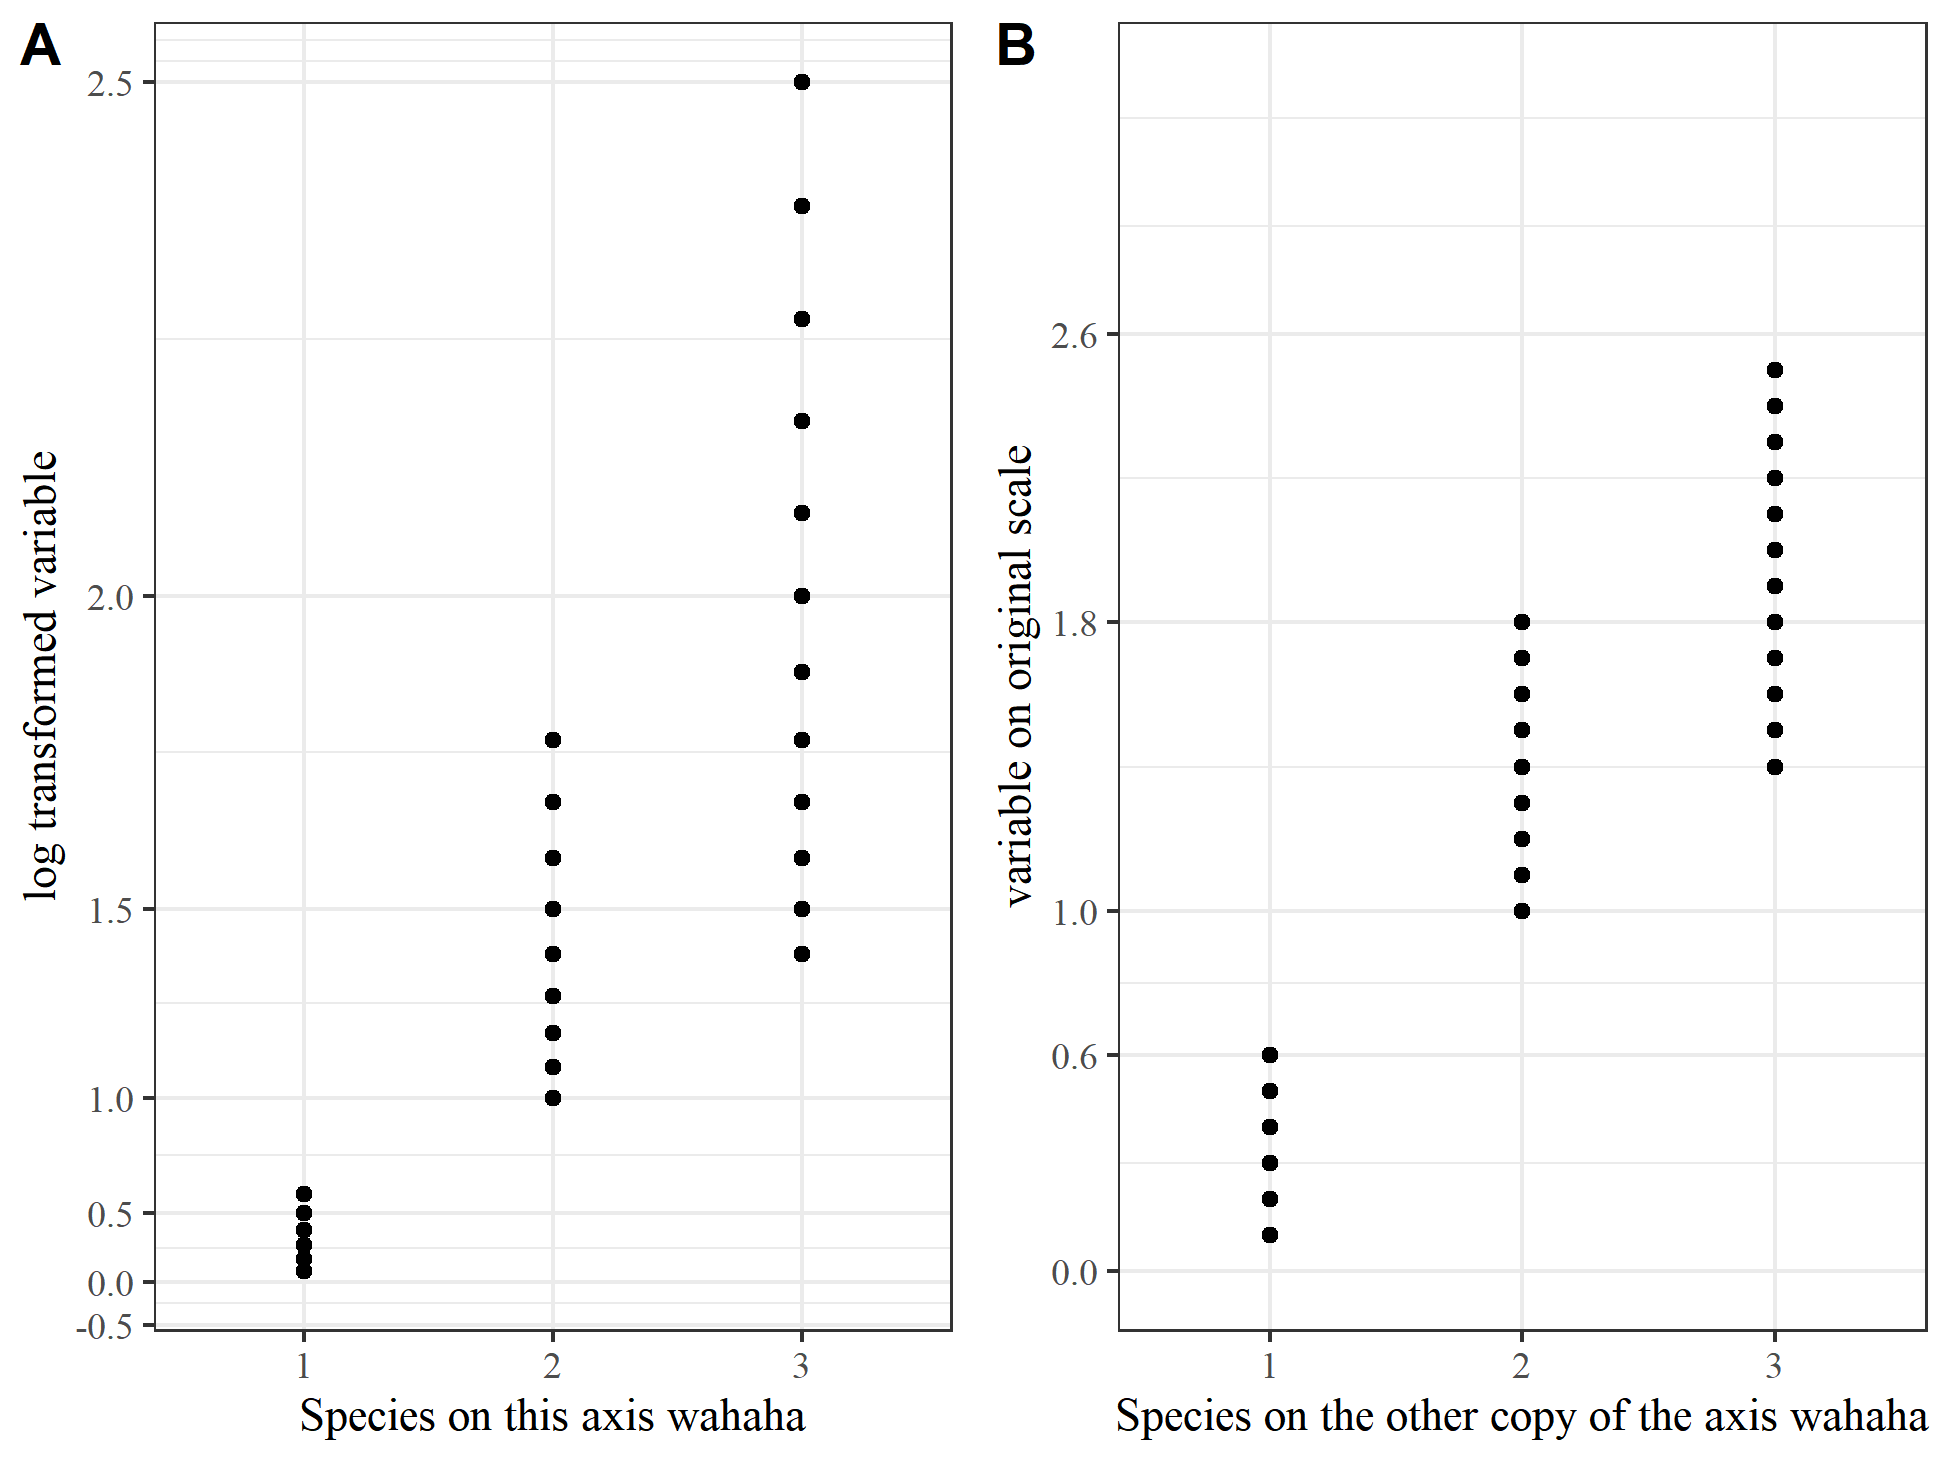
\includegraphics[width=0.9\linewidth]{cookbook_files/figure-latex/two_log_norm_plot-1} 

}

\caption{Title of the plot above}\label{fig:two_log_norm_plot}
\end{figure}

\newpage

\hypertarget{side-by-side-different-graphs-different-fig.-title}{%
\subsubsection{Side by side different graphs, different
fig.~title}\label{side-by-side-different-graphs-different-fig.-title}}

\begin{figure}[h]
\begin{multicols}{2}
\begin{figure}[H]
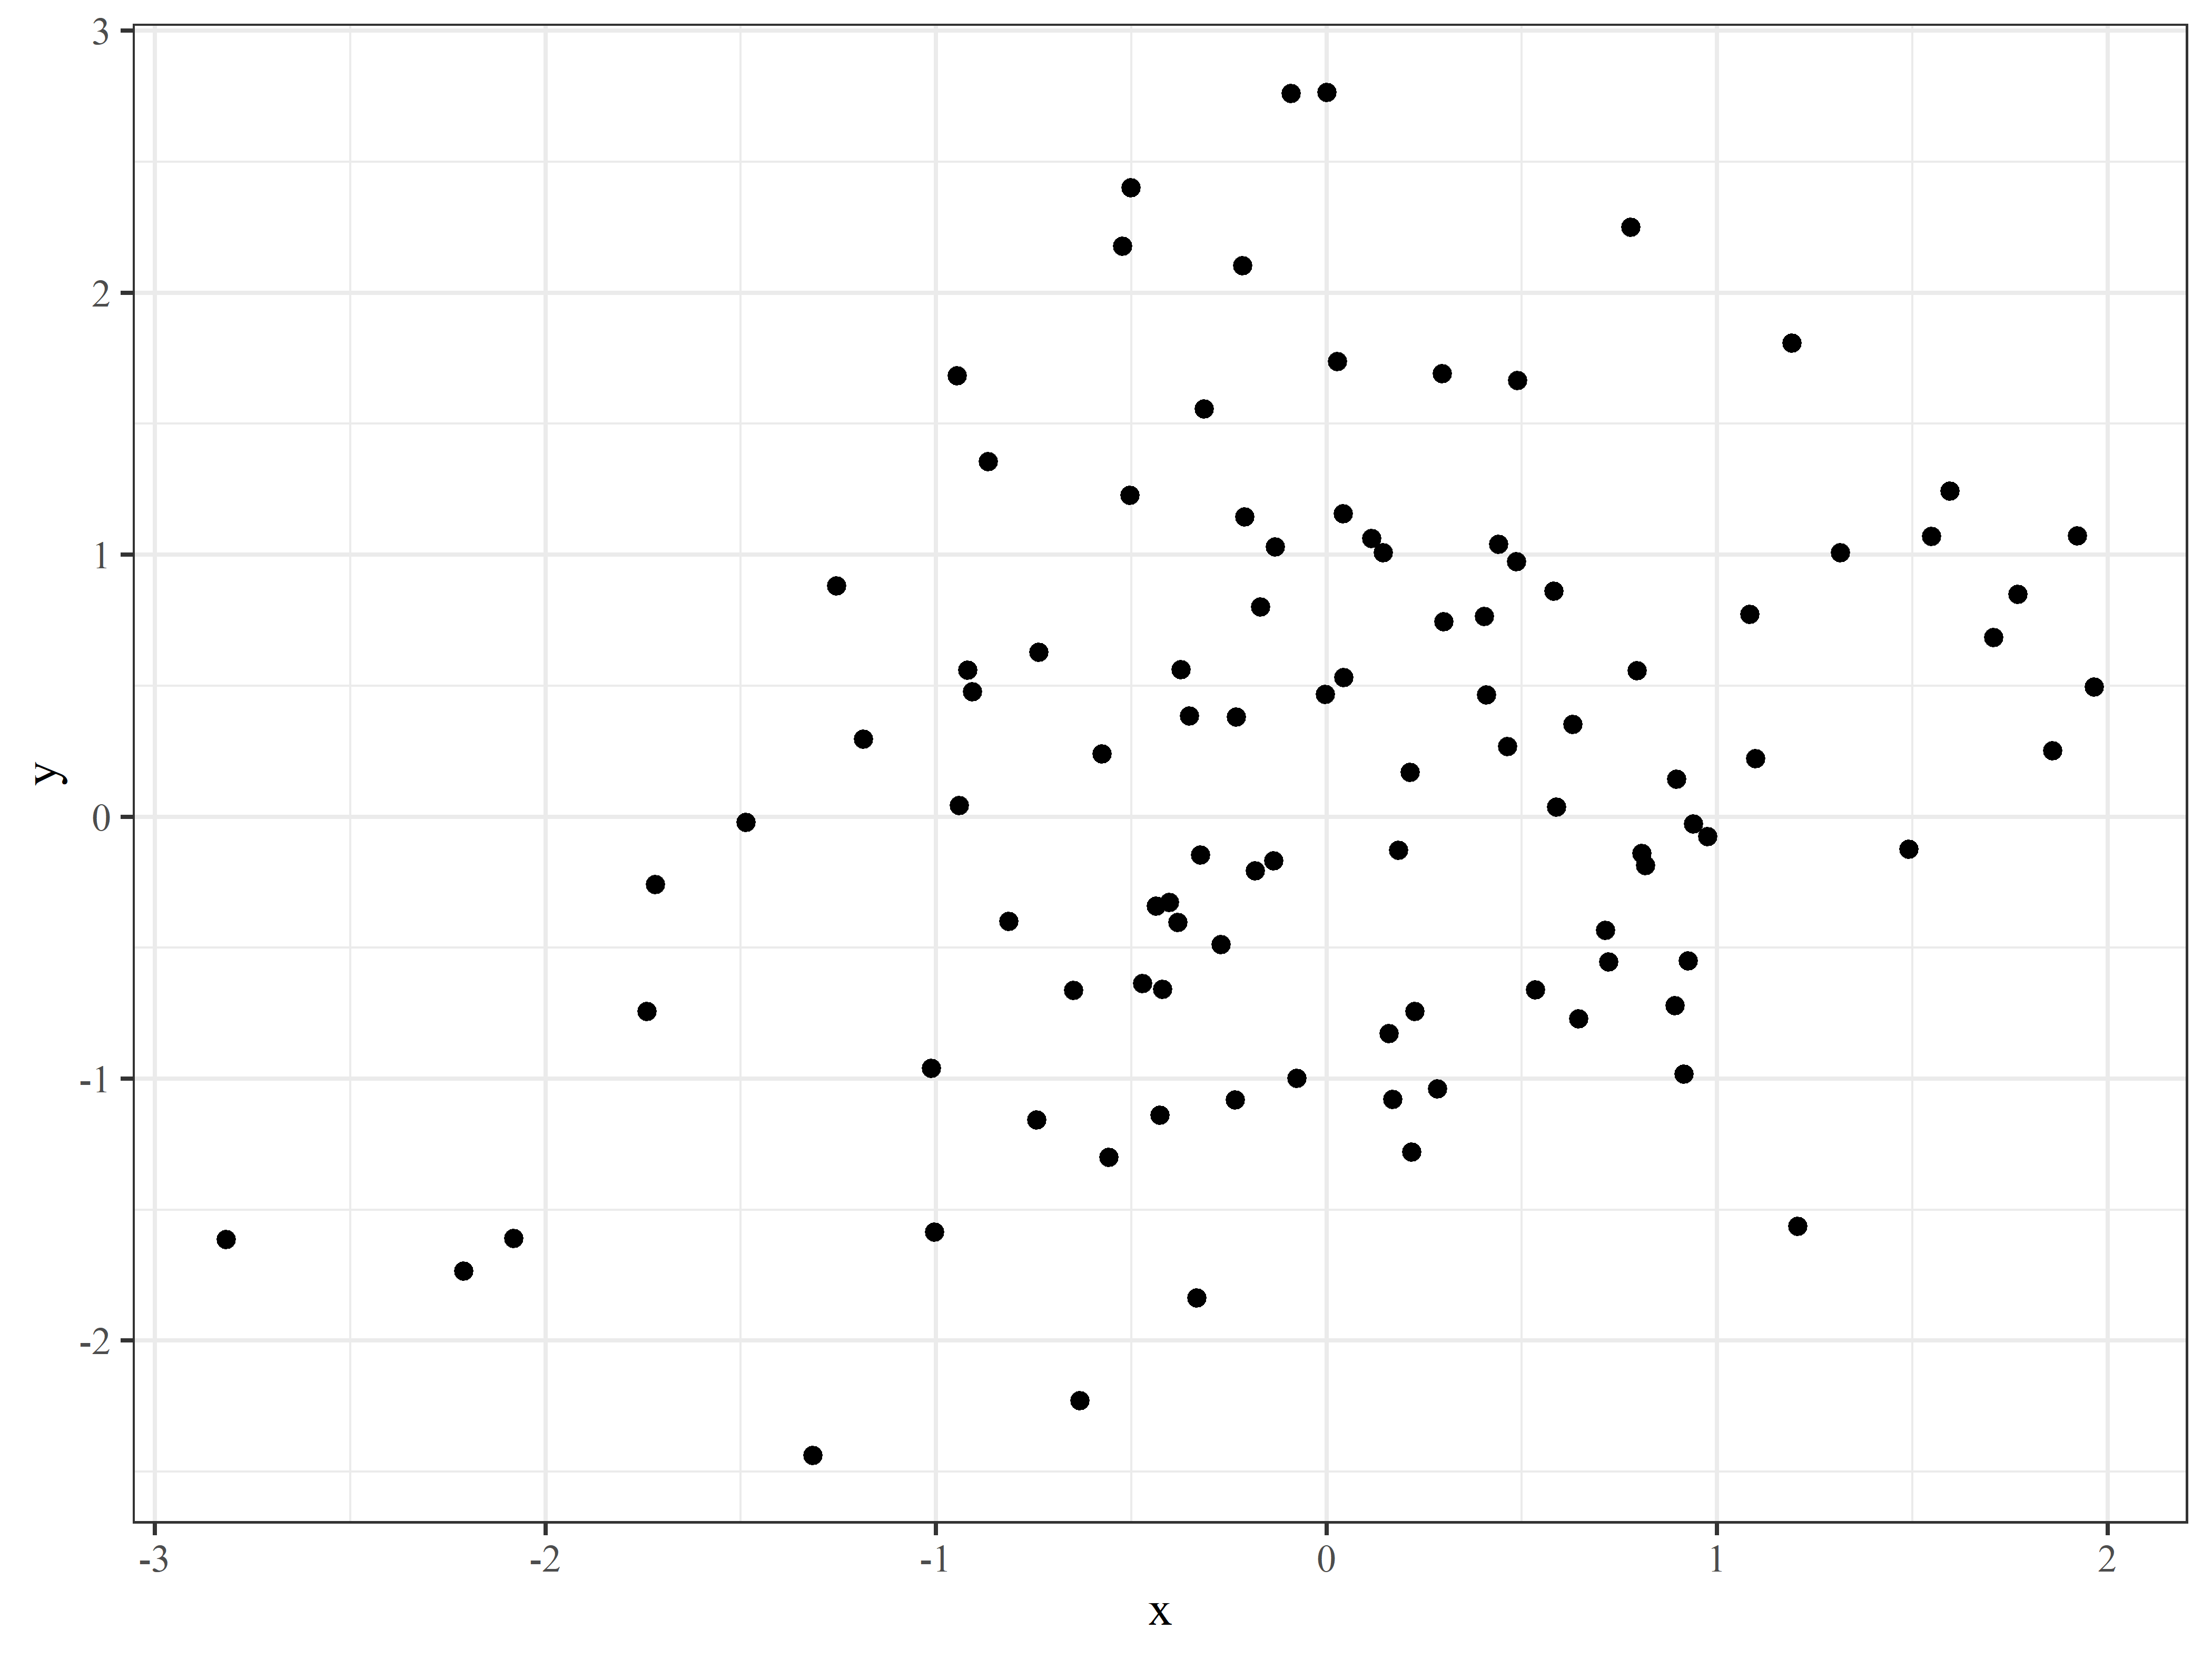
\includegraphics[width = \linewidth]{mandatory_chunk_name-1.png}
\caption{Plot the first}
\label{fig:plotmeans}
\end{figure}

\columnbreak

\begin{figure}[H]
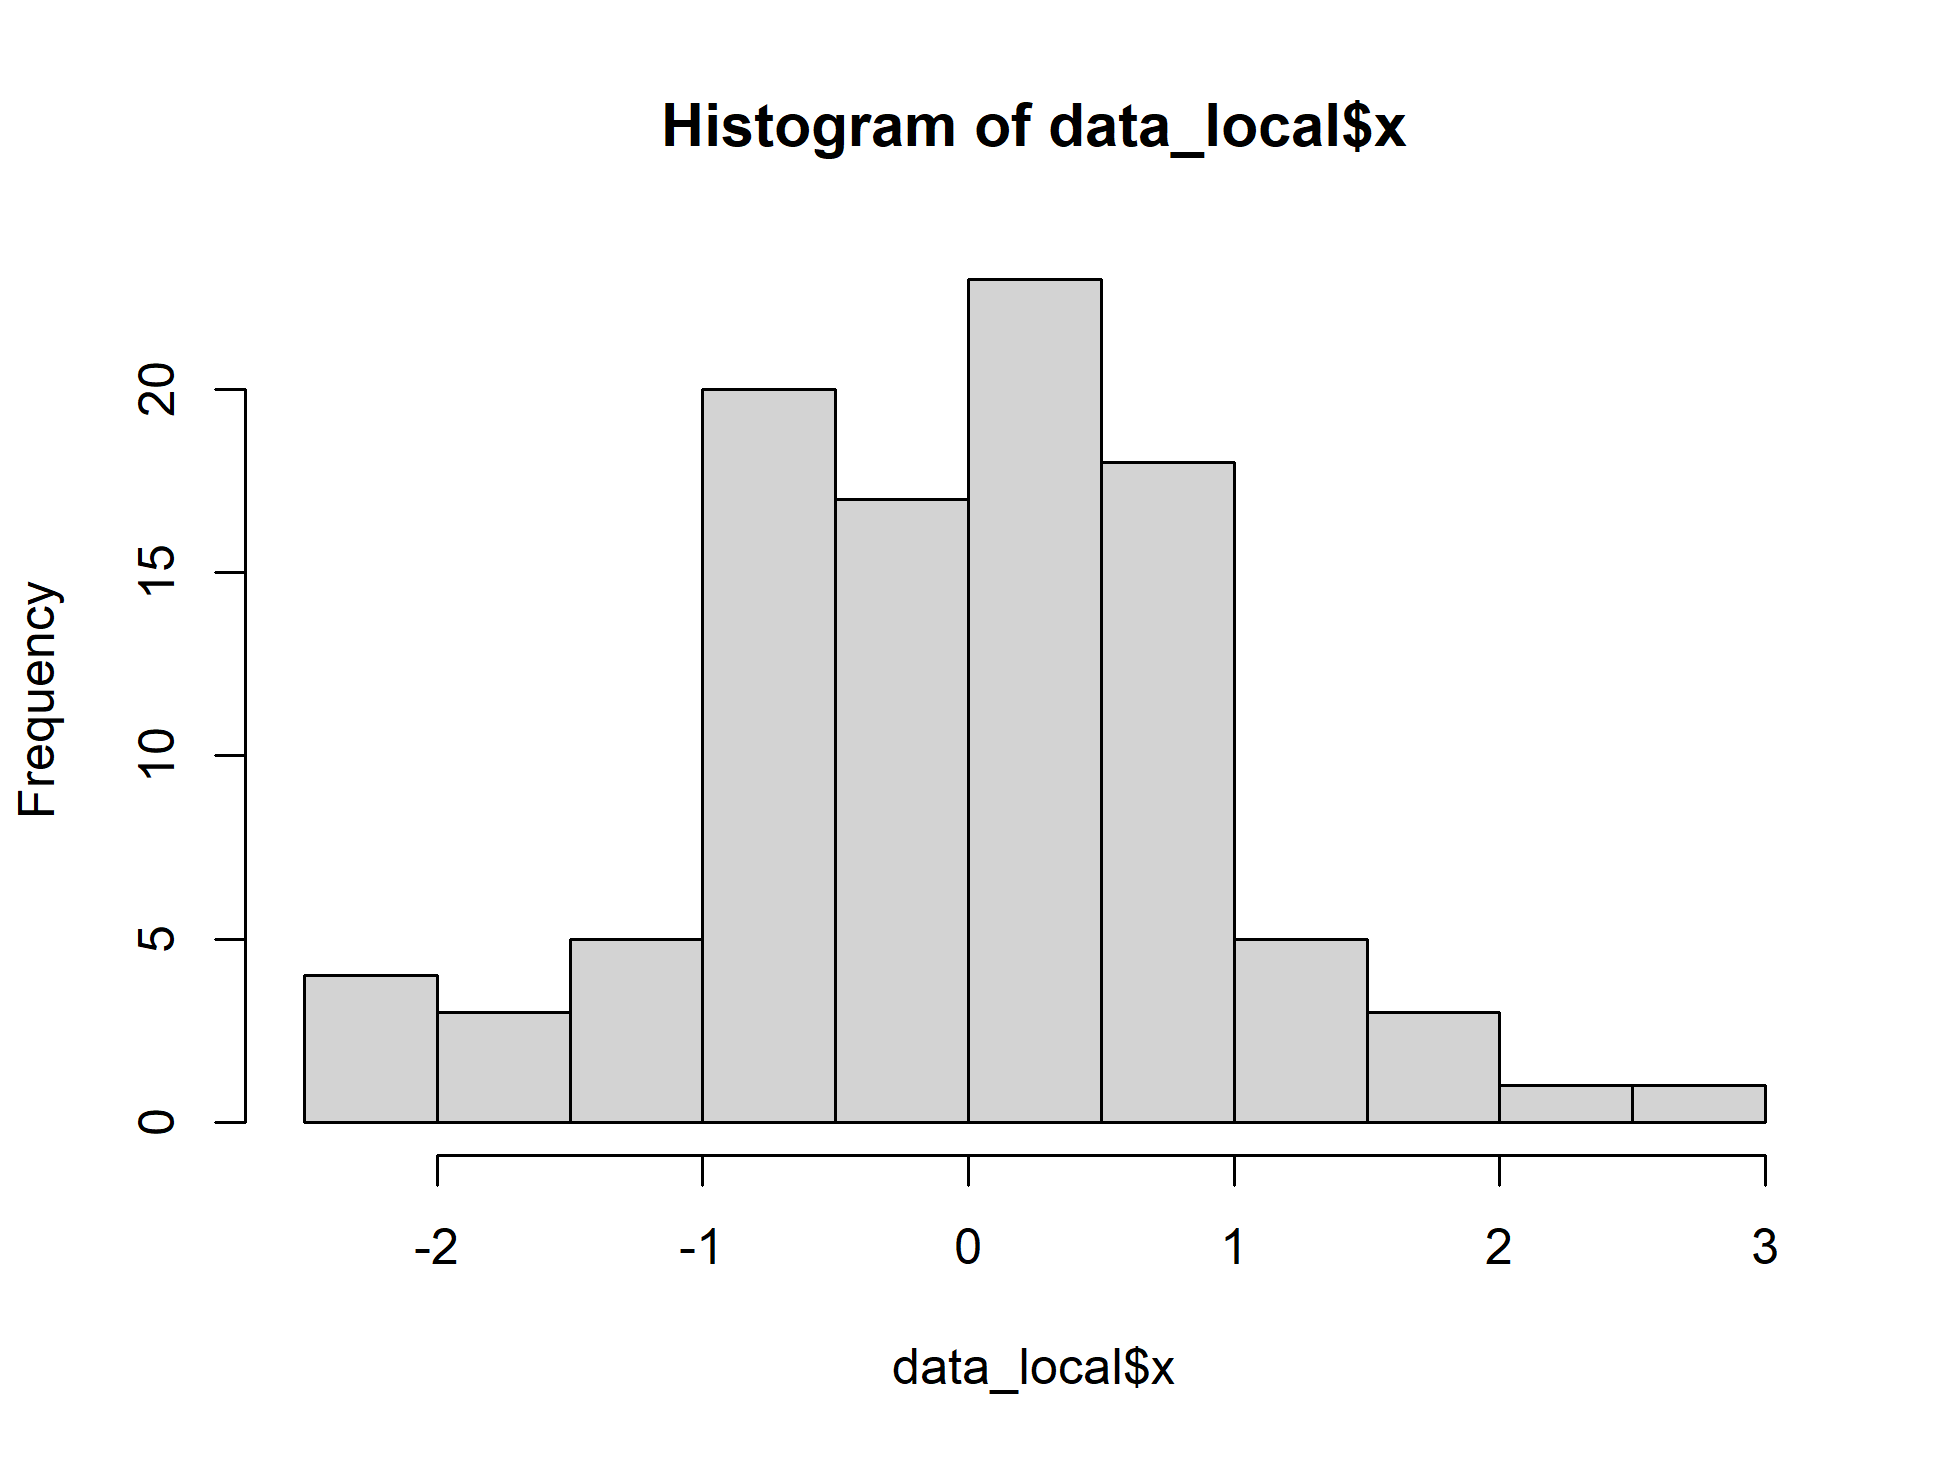
\includegraphics[width = \linewidth]{mandatory_chunk_name-2.png}
\centering
\caption{Plot the second}
\label{fig:histogram}
\end{figure}
\end{multicols}
\end{figure}

\newpage

\hypertarget{a-tbl_summary-example}{%
\subsubsection{A tbl\_summary example}\label{a-tbl_summary-example}}

Lorem ipsum dolor sit amet, consectetur adipiscing elit. Maecenas et
justo non erat lobortis tincidunt. In et nunc sollicitudin, pellentesque
neque sit amet, blandit mauris. Praesent nunc urna, mattis non risus eu,
egestas bibendum nunc. Mauris et hendrerit purus. Morbi posuere nibh
erat, vel dignissim nisl fermentum sed. Vivamus nisi tellus, placerat
vitae accumsan nec, tincidunt ac leo. Phasellus sed dolor et massa
placerat sodales. Nulla facilisi. Sed sed justo nec lacus egestas
malesuada hendrerit quis ligula. Vestibulum in purus mattis, elementum
quam sit amet, eleifend lorem. Nunc dictum ligula ante, sit amet auctor
nisi aliquet non. Donec ullamcorper ultrices molestie.

Nunc sodales, massa ut vehicula auctor, augue felis faucibus urna, et
semper libero tortor accumsan magna. Proin non tortor quis erat tempor
fermentum et ut tortor. Praesent elementum tristique sapien a interdum.
Aenean sit amet mi a sapien semper ullamcorper. Phasellus quis enim
tempor, porttitor odio eu, faucibus libero. Nullam eu eros vitae eros
dictum luctus. Mauris congue ante vel laoreet eleifend.

Nunc lobortis sapien ac eros venenatis commodo. Vestibulum a venenatis
enim. Sed sit amet lectus gravida quam mollis porttitor eu ut elit.
Etiam dolor massa, dignissim et facilisis vitae, congue ac sem. Proin
sed sem condimentum, tincidunt sapien eget, accumsan dolor. Aenean
varius mi ligula, nec scelerisque ligula dignissim ac. Cras ex magna,
feugiat sed libero sed, vestibulum condimentum risus. Sed pretium
maximus est, quis imperdiet purus consectetur vestibulum. Phasellus
mattis sapien ante, convallis facilisis mi posuere quis. Maecenas id
magna scelerisque, ultrices sem viverra, ornare lectus. Ut consectetur
eleifend tortor sagittis venenatis. Cras quis lorem et odio tristique
gravida. Sed sapien justo, euismod id ligula quis, fringilla egestas
nulla. Aenean molestie felis ut aliquam scelerisque. Maecenas id ligula
ultricies, tristique sem eu, eleifend est. Cras tempor feugiat nibh sit
amet efficitur.

 
  \providecommand{\huxb}[2]{\arrayrulecolor[RGB]{#1}\global\arrayrulewidth=#2pt}
  \providecommand{\huxvb}[2]{\color[RGB]{#1}\vrule width #2pt}
  \providecommand{\huxtpad}[1]{\rule{0pt}{#1}}
  \providecommand{\huxbpad}[1]{\rule[-#1]{0pt}{#1}}

\begin{table}[h]
\begin{centerbox}
\begin{threeparttable}
\captionsetup{justification=centering,singlelinecheck=off}
\caption{Plot without much thought or meaning}
 \label{tab:unnamed-chunk-8}
\setlength{\tabcolsep}{0pt}
\begin{tabularx}{0.4\textwidth}{p{0.1\textwidth} p{0.1\textwidth} p{0.1\textwidth} p{0.1\textwidth}}


\hhline{>{\huxb{0, 0, 0}{0.8}}->{\huxb{0, 0, 0}{0.8}}->{\huxb{0, 0, 0}{0.8}}->{\huxb{0, 0, 0}{0.8}}-}
\arrayrulecolor{black}

\multicolumn{1}{!{\huxvb{0, 0, 0}{0.8}}m{0.1\textwidth}!{\huxvb{0, 0, 0}{0.8}}}{\cellcolor[RGB]{204, 204, 204}\hspace{6pt}\parbox[c]{0.1\textwidth-6pt-6pt}{\huxtpad{6pt + 1em}\raggedright \textbf{{\fontsize{7pt}{8.4pt}\selectfont 
}}\huxbpad{6pt}}} &
\multicolumn{1}{m{0.1\textwidth}!{\huxvb{0, 0, 0}{0.8}}}{\cellcolor[RGB]{204, 204, 204}\hspace{6pt}\parbox[c]{0.1\textwidth-6pt-6pt}{\huxtpad{6pt + 1em}\centering \textbf{{\fontsize{7pt}{8.4pt}\selectfont \textbf{Setosa}, N = 50
}}\huxbpad{6pt}}} &
\multicolumn{1}{m{0.1\textwidth}!{\huxvb{0, 0, 0}{0.8}}}{\cellcolor[RGB]{204, 204, 204}\hspace{6pt}\parbox[c]{0.1\textwidth-6pt-6pt}{\huxtpad{6pt + 1em}\centering \textbf{{\fontsize{7pt}{8.4pt}\selectfont \textbf{Verginica}, N = 50
}}\huxbpad{6pt}}} &
\multicolumn{1}{m{0.1\textwidth}!{\huxvb{0, 0, 0}{0.8}}}{\cellcolor[RGB]{204, 204, 204}\hspace{6pt}\parbox[c]{0.1\textwidth-6pt-6pt}{\huxtpad{6pt + 1em}\centering \textbf{{\fontsize{7pt}{8.4pt}\selectfont \textbf{Versicolor}, N = 50
}}\huxbpad{6pt}}} \tabularnewline[-0.5pt]


\hhline{>{\huxb{0, 0, 0}{0.8}}->{\huxb{0, 0, 0}{0.8}}->{\huxb{0, 0, 0}{0.8}}->{\huxb{0, 0, 0}{0.8}}-}
\arrayrulecolor{black}

\multicolumn{1}{!{\huxvb{0, 0, 0}{0.8}}m{0.1\textwidth}!{\huxvb{0, 0, 0}{0.8}}}{\cellcolor[RGB]{242, 242, 242}\hspace{6pt}\parbox[c]{0.1\textwidth-6pt-6pt}{\huxtpad{6pt + 1em}\raggedright \textbf{{\fontsize{7pt}{8.4pt}\selectfont Numeric representation of species}}\huxbpad{6pt}}} &
\multicolumn{1}{m{0.1\textwidth}!{\huxvb{0, 0, 0}{0.8}}}{\cellcolor[RGB]{242, 242, 242}\hspace{6pt}\parbox[c]{0.1\textwidth-6pt-6pt}{\huxtpad{6pt + 1em}\centering {\fontsize{7pt}{8.4pt}\selectfont }\huxbpad{6pt}}} &
\multicolumn{1}{m{0.1\textwidth}!{\huxvb{0, 0, 0}{0.8}}}{\cellcolor[RGB]{242, 242, 242}\hspace{6pt}\parbox[c]{0.1\textwidth-6pt-6pt}{\huxtpad{6pt + 1em}\centering {\fontsize{7pt}{8.4pt}\selectfont }\huxbpad{6pt}}} &
\multicolumn{1}{m{0.1\textwidth}!{\huxvb{0, 0, 0}{0.8}}}{\cellcolor[RGB]{242, 242, 242}\hspace{6pt}\parbox[c]{0.1\textwidth-6pt-6pt}{\huxtpad{6pt + 1em}\centering {\fontsize{7pt}{8.4pt}\selectfont }\huxbpad{6pt}}} \tabularnewline[-0.5pt]


\hhline{>{\huxb{0, 0, 0}{0.8}}->{\huxb{0, 0, 0}{0.8}}->{\huxb{0, 0, 0}{0.8}}->{\huxb{0, 0, 0}{0.8}}-}
\arrayrulecolor{black}

\multicolumn{1}{!{\huxvb{0, 0, 0}{0.8}}m{0.1\textwidth}!{\huxvb{0, 0, 0}{0.8}}}{\cellcolor[RGB]{230, 230, 230}\hspace{6pt}\parbox[c]{0.1\textwidth-6pt-6pt}{\huxtpad{6pt + 1em}\raggedright \textit{{\fontsize{7pt}{8.4pt}\selectfont 1}}\huxbpad{6pt}}} &
\multicolumn{1}{m{0.1\textwidth}!{\huxvb{0, 0, 0}{0.8}}}{\cellcolor[RGB]{230, 230, 230}\hspace{6pt}\parbox[c]{0.1\textwidth-6pt-6pt}{\huxtpad{6pt + 1em}\centering {\fontsize{7pt}{8.4pt}\selectfont 50 (100\%)}\huxbpad{6pt}}} &
\multicolumn{1}{m{0.1\textwidth}!{\huxvb{0, 0, 0}{0.8}}}{\cellcolor[RGB]{230, 230, 230}\hspace{6pt}\parbox[c]{0.1\textwidth-6pt-6pt}{\huxtpad{6pt + 1em}\centering {\fontsize{7pt}{8.4pt}\selectfont 0 (0\%)}\huxbpad{6pt}}} &
\multicolumn{1}{m{0.1\textwidth}!{\huxvb{0, 0, 0}{0.8}}}{\cellcolor[RGB]{230, 230, 230}\hspace{6pt}\parbox[c]{0.1\textwidth-6pt-6pt}{\huxtpad{6pt + 1em}\centering {\fontsize{7pt}{8.4pt}\selectfont 0 (0\%)}\huxbpad{6pt}}} \tabularnewline[-0.5pt]


\hhline{>{\huxb{0, 0, 0}{0.8}}->{\huxb{0, 0, 0}{0.8}}->{\huxb{0, 0, 0}{0.8}}->{\huxb{0, 0, 0}{0.8}}-}
\arrayrulecolor{black}

\multicolumn{1}{!{\huxvb{0, 0, 0}{0.8}}m{0.1\textwidth}!{\huxvb{0, 0, 0}{0.8}}}{\cellcolor[RGB]{242, 242, 242}\hspace{6pt}\parbox[c]{0.1\textwidth-6pt-6pt}{\huxtpad{6pt + 1em}\raggedright \textit{{\fontsize{7pt}{8.4pt}\selectfont 2}}\huxbpad{6pt}}} &
\multicolumn{1}{m{0.1\textwidth}!{\huxvb{0, 0, 0}{0.8}}}{\cellcolor[RGB]{242, 242, 242}\hspace{6pt}\parbox[c]{0.1\textwidth-6pt-6pt}{\huxtpad{6pt + 1em}\centering {\fontsize{7pt}{8.4pt}\selectfont 0 (0\%)}\huxbpad{6pt}}} &
\multicolumn{1}{m{0.1\textwidth}!{\huxvb{0, 0, 0}{0.8}}}{\cellcolor[RGB]{242, 242, 242}\hspace{6pt}\parbox[c]{0.1\textwidth-6pt-6pt}{\huxtpad{6pt + 1em}\centering {\fontsize{7pt}{8.4pt}\selectfont 0 (0\%)}\huxbpad{6pt}}} &
\multicolumn{1}{m{0.1\textwidth}!{\huxvb{0, 0, 0}{0.8}}}{\cellcolor[RGB]{242, 242, 242}\hspace{6pt}\parbox[c]{0.1\textwidth-6pt-6pt}{\huxtpad{6pt + 1em}\centering {\fontsize{7pt}{8.4pt}\selectfont 50 (100\%)}\huxbpad{6pt}}} \tabularnewline[-0.5pt]


\hhline{>{\huxb{0, 0, 0}{0.8}}->{\huxb{0, 0, 0}{0.8}}->{\huxb{0, 0, 0}{0.8}}->{\huxb{0, 0, 0}{0.8}}-}
\arrayrulecolor{black}

\multicolumn{1}{!{\huxvb{0, 0, 0}{0.8}}m{0.1\textwidth}!{\huxvb{0, 0, 0}{0.8}}}{\cellcolor[RGB]{230, 230, 230}\hspace{6pt}\parbox[c]{0.1\textwidth-6pt-6pt}{\huxtpad{6pt + 1em}\raggedright \textit{{\fontsize{7pt}{8.4pt}\selectfont 3}}\huxbpad{6pt}}} &
\multicolumn{1}{m{0.1\textwidth}!{\huxvb{0, 0, 0}{0.8}}}{\cellcolor[RGB]{230, 230, 230}\hspace{6pt}\parbox[c]{0.1\textwidth-6pt-6pt}{\huxtpad{6pt + 1em}\centering {\fontsize{7pt}{8.4pt}\selectfont 0 (0\%)}\huxbpad{6pt}}} &
\multicolumn{1}{m{0.1\textwidth}!{\huxvb{0, 0, 0}{0.8}}}{\cellcolor[RGB]{230, 230, 230}\hspace{6pt}\parbox[c]{0.1\textwidth-6pt-6pt}{\huxtpad{6pt + 1em}\centering {\fontsize{7pt}{8.4pt}\selectfont 50 (100\%)}\huxbpad{6pt}}} &
\multicolumn{1}{m{0.1\textwidth}!{\huxvb{0, 0, 0}{0.8}}}{\cellcolor[RGB]{230, 230, 230}\hspace{6pt}\parbox[c]{0.1\textwidth-6pt-6pt}{\huxtpad{6pt + 1em}\centering {\fontsize{7pt}{8.4pt}\selectfont 0 (0\%)}\huxbpad{6pt}}} \tabularnewline[-0.5pt]


\hhline{>{\huxb{0, 0, 0}{0.8}}->{\huxb{0, 0, 0}{0.8}}->{\huxb{0, 0, 0}{0.8}}->{\huxb{0, 0, 0}{0.8}}-}
\arrayrulecolor{black}

\multicolumn{1}{!{\huxvb{0, 0, 0}{0.8}}m{0.1\textwidth}!{\huxvb{0, 0, 0}{0.8}}}{\cellcolor[RGB]{242, 242, 242}\hspace{6pt}\parbox[c]{0.1\textwidth-6pt-6pt}{\huxtpad{6pt + 1em}\raggedright \textbf{{\fontsize{7pt}{8.4pt}\selectfont These are the width of the petals}}\huxbpad{6pt}}} &
\multicolumn{1}{m{0.1\textwidth}!{\huxvb{0, 0, 0}{0.8}}}{\cellcolor[RGB]{242, 242, 242}\hspace{6pt}\parbox[c]{0.1\textwidth-6pt-6pt}{\huxtpad{6pt + 1em}\centering {\fontsize{7pt}{8.4pt}\selectfont 0.20 (0.20, 0.30)}\huxbpad{6pt}}} &
\multicolumn{1}{m{0.1\textwidth}!{\huxvb{0, 0, 0}{0.8}}}{\cellcolor[RGB]{242, 242, 242}\hspace{6pt}\parbox[c]{0.1\textwidth-6pt-6pt}{\huxtpad{6pt + 1em}\centering {\fontsize{7pt}{8.4pt}\selectfont 2.00 (1.80, 2.30)}\huxbpad{6pt}}} &
\multicolumn{1}{m{0.1\textwidth}!{\huxvb{0, 0, 0}{0.8}}}{\cellcolor[RGB]{242, 242, 242}\hspace{6pt}\parbox[c]{0.1\textwidth-6pt-6pt}{\huxtpad{6pt + 1em}\centering {\fontsize{7pt}{8.4pt}\selectfont 1.30 (1.20, 1.50)}\huxbpad{6pt}}} \tabularnewline[-0.5pt]


\hhline{>{\huxb{0, 0, 0}{0.8}}->{\huxb{0, 0, 0}{0.8}}->{\huxb{0, 0, 0}{0.8}}->{\huxb{0, 0, 0}{0.8}}-}
\arrayrulecolor{black}

\multicolumn{1}{!{\huxvb{0, 0, 0}{0.8}}m{0.1\textwidth}!{\huxvb{0, 0, 0}{0.8}}}{\cellcolor[RGB]{230, 230, 230}\hspace{6pt}\parbox[c]{0.1\textwidth-6pt-6pt}{\huxtpad{6pt + 1em}\raggedright \textbf{{\fontsize{7pt}{8.4pt}\selectfont These are the length of the petals}}\huxbpad{6pt}}} &
\multicolumn{1}{m{0.1\textwidth}!{\huxvb{0, 0, 0}{0.8}}}{\cellcolor[RGB]{230, 230, 230}\hspace{6pt}\parbox[c]{0.1\textwidth-6pt-6pt}{\huxtpad{6pt + 1em}\centering {\fontsize{7pt}{8.4pt}\selectfont 1.50 (1.40, 1.58)}\huxbpad{6pt}}} &
\multicolumn{1}{m{0.1\textwidth}!{\huxvb{0, 0, 0}{0.8}}}{\cellcolor[RGB]{230, 230, 230}\hspace{6pt}\parbox[c]{0.1\textwidth-6pt-6pt}{\huxtpad{6pt + 1em}\centering {\fontsize{7pt}{8.4pt}\selectfont 5.55 (5.10, 5.88)}\huxbpad{6pt}}} &
\multicolumn{1}{m{0.1\textwidth}!{\huxvb{0, 0, 0}{0.8}}}{\cellcolor[RGB]{230, 230, 230}\hspace{6pt}\parbox[c]{0.1\textwidth-6pt-6pt}{\huxtpad{6pt + 1em}\centering {\fontsize{7pt}{8.4pt}\selectfont 4.35 (4.00, 4.60)}\huxbpad{6pt}}} \tabularnewline[-0.5pt]


\hhline{>{\huxb{0, 0, 0}{0.8}}->{\huxb{0, 0, 0}{0.8}}->{\huxb{0, 0, 0}{0.8}}->{\huxb{0, 0, 0}{0.8}}-}
\arrayrulecolor{black}

\multicolumn{1}{!{\huxvb{0, 0, 0}{0.8}}m{0.1\textwidth}!{\huxvb{0, 0, 0}{0.8}}}{\cellcolor[RGB]{242, 242, 242}\hspace{6pt}\parbox[c]{0.1\textwidth-6pt-6pt}{\huxtpad{6pt + 1em}\raggedright \textbf{{\fontsize{7pt}{8.4pt}\selectfont These are the width of the sepals}}\huxbpad{6pt}}} &
\multicolumn{1}{m{0.1\textwidth}!{\huxvb{0, 0, 0}{0.8}}}{\cellcolor[RGB]{242, 242, 242}\hspace{6pt}\parbox[c]{0.1\textwidth-6pt-6pt}{\huxtpad{6pt + 1em}\centering {\fontsize{7pt}{8.4pt}\selectfont 3.40 (3.20, 3.68)}\huxbpad{6pt}}} &
\multicolumn{1}{m{0.1\textwidth}!{\huxvb{0, 0, 0}{0.8}}}{\cellcolor[RGB]{242, 242, 242}\hspace{6pt}\parbox[c]{0.1\textwidth-6pt-6pt}{\huxtpad{6pt + 1em}\centering {\fontsize{7pt}{8.4pt}\selectfont 3.00 (2.80, 3.18)}\huxbpad{6pt}}} &
\multicolumn{1}{m{0.1\textwidth}!{\huxvb{0, 0, 0}{0.8}}}{\cellcolor[RGB]{242, 242, 242}\hspace{6pt}\parbox[c]{0.1\textwidth-6pt-6pt}{\huxtpad{6pt + 1em}\centering {\fontsize{7pt}{8.4pt}\selectfont 2.80 (2.53, 3.00)}\huxbpad{6pt}}} \tabularnewline[-0.5pt]


\hhline{>{\huxb{0, 0, 0}{0.8}}->{\huxb{0, 0, 0}{0.8}}->{\huxb{0, 0, 0}{0.8}}->{\huxb{0, 0, 0}{0.8}}-}
\arrayrulecolor{black}

\multicolumn{1}{!{\huxvb{0, 0, 0}{0.8}}m{0.1\textwidth}!{\huxvb{0, 0, 0}{0.8}}}{\cellcolor[RGB]{230, 230, 230}\hspace{6pt}\parbox[c]{0.1\textwidth-6pt-6pt}{\huxtpad{6pt + 1em}\raggedright \textbf{{\fontsize{7pt}{8.4pt}\selectfont These are the length of the sepals}}\huxbpad{6pt}}} &
\multicolumn{1}{m{0.1\textwidth}!{\huxvb{0, 0, 0}{0.8}}}{\cellcolor[RGB]{230, 230, 230}\hspace{6pt}\parbox[c]{0.1\textwidth-6pt-6pt}{\huxtpad{6pt + 1em}\centering {\fontsize{7pt}{8.4pt}\selectfont 5.00 (4.80, 5.20)}\huxbpad{6pt}}} &
\multicolumn{1}{m{0.1\textwidth}!{\huxvb{0, 0, 0}{0.8}}}{\cellcolor[RGB]{230, 230, 230}\hspace{6pt}\parbox[c]{0.1\textwidth-6pt-6pt}{\huxtpad{6pt + 1em}\centering {\fontsize{7pt}{8.4pt}\selectfont 6.50 (6.23, 6.90)}\huxbpad{6pt}}} &
\multicolumn{1}{m{0.1\textwidth}!{\huxvb{0, 0, 0}{0.8}}}{\cellcolor[RGB]{230, 230, 230}\hspace{6pt}\parbox[c]{0.1\textwidth-6pt-6pt}{\huxtpad{6pt + 1em}\centering {\fontsize{7pt}{8.4pt}\selectfont 5.90 (5.60, 6.30)}\huxbpad{6pt}}} \tabularnewline[-0.5pt]


\hhline{>{\huxb{0, 0, 0}{0.8}}->{\huxb{0, 0, 0}{0.8}}->{\huxb{0, 0, 0}{0.8}}->{\huxb{0, 0, 0}{0.8}}-}
\arrayrulecolor{black}

\multicolumn{1}{!{\huxvb{0, 0, 0}{0.8}}m{0.1\textwidth}!{\huxvb{0, 0, 0}{0.8}}}{\cellcolor[RGB]{242, 242, 242}\hspace{6pt}\parbox[c]{0.1\textwidth-6pt-6pt}{\huxtpad{6pt + 1em}\raggedright \textbf{{\fontsize{7pt}{8.4pt}\selectfont This is a date column to illustrate transformations}}\huxbpad{6pt}}} &
\multicolumn{1}{m{0.1\textwidth}!{\huxvb{0, 0, 0}{0.8}}}{\cellcolor[RGB]{242, 242, 242}\hspace{6pt}\parbox[c]{0.1\textwidth-6pt-6pt}{\huxtpad{6pt + 1em}\centering {\fontsize{7pt}{8.4pt}\selectfont 2022-01-01 to 2022-02-19}\huxbpad{6pt}}} &
\multicolumn{1}{m{0.1\textwidth}!{\huxvb{0, 0, 0}{0.8}}}{\cellcolor[RGB]{242, 242, 242}\hspace{6pt}\parbox[c]{0.1\textwidth-6pt-6pt}{\huxtpad{6pt + 1em}\centering {\fontsize{7pt}{8.4pt}\selectfont 2022-04-11 to 2022-05-30}\huxbpad{6pt}}} &
\multicolumn{1}{m{0.1\textwidth}!{\huxvb{0, 0, 0}{0.8}}}{\cellcolor[RGB]{242, 242, 242}\hspace{6pt}\parbox[c]{0.1\textwidth-6pt-6pt}{\huxtpad{6pt + 1em}\centering {\fontsize{7pt}{8.4pt}\selectfont 2022-02-20 to 2022-04-10}\huxbpad{6pt}}} \tabularnewline[-0.5pt]


\hhline{>{\huxb{0, 0, 0}{0.8}}->{\huxb{0, 0, 0}{0.8}}->{\huxb{0, 0, 0}{0.8}}->{\huxb{0, 0, 0}{0.8}}-}
\arrayrulecolor{black}

\multicolumn{1}{!{\huxvb{0, 0, 0}{0.8}}m{0.1\textwidth}!{\huxvb{0, 0, 0}{0.8}}}{\cellcolor[RGB]{230, 230, 230}\hspace{6pt}\parbox[c]{0.1\textwidth-6pt-6pt}{\huxtpad{6pt + 1em}\raggedright \textbf{{\fontsize{7pt}{8.4pt}\selectfont This is my new example variable, adding up the lengths}}\huxbpad{6pt}}} &
\multicolumn{1}{m{0.1\textwidth}!{\huxvb{0, 0, 0}{0.8}}}{\cellcolor[RGB]{230, 230, 230}\hspace{6pt}\parbox[c]{0.1\textwidth-6pt-6pt}{\huxtpad{6pt + 1em}\centering {\fontsize{7pt}{8.4pt}\selectfont 3.70 (3.40, 3.90)}\huxbpad{6pt}}} &
\multicolumn{1}{m{0.1\textwidth}!{\huxvb{0, 0, 0}{0.8}}}{\cellcolor[RGB]{230, 230, 230}\hspace{6pt}\parbox[c]{0.1\textwidth-6pt-6pt}{\huxtpad{6pt + 1em}\centering {\fontsize{7pt}{8.4pt}\selectfont 4.95 (4.63, 5.38)}\huxbpad{6pt}}} &
\multicolumn{1}{m{0.1\textwidth}!{\huxvb{0, 0, 0}{0.8}}}{\cellcolor[RGB]{230, 230, 230}\hspace{6pt}\parbox[c]{0.1\textwidth-6pt-6pt}{\huxtpad{6pt + 1em}\centering {\fontsize{7pt}{8.4pt}\selectfont 4.20 (3.73, 4.40)}\huxbpad{6pt}}} \tabularnewline[-0.5pt]


\hhline{>{\huxb{0, 0, 0}{0.8}}->{\huxb{0, 0, 0}{0.8}}->{\huxb{0, 0, 0}{0.8}}->{\huxb{0, 0, 0}{0.8}}-}
\arrayrulecolor{black}

\multicolumn{1}{!{\huxvb{0, 0, 0}{0.8}}m{0.1\textwidth}!{\huxvb{0, 0, 0}{0.8}}}{\cellcolor[RGB]{242, 242, 242}\hspace{6pt}\parbox[c]{0.1\textwidth-6pt-6pt}{\huxtpad{6pt + 1em}\raggedright \textbf{{\fontsize{7pt}{8.4pt}\selectfont mock\_ID}}\huxbpad{6pt}}} &
\multicolumn{1}{m{0.1\textwidth}!{\huxvb{0, 0, 0}{0.8}}}{\cellcolor[RGB]{242, 242, 242}\hspace{6pt}\parbox[c]{0.1\textwidth-6pt-6pt}{\huxtpad{6pt + 1em}\centering {\fontsize{7pt}{8.4pt}\selectfont 8.5 (5.0, 14.0)}\huxbpad{6pt}}} &
\multicolumn{1}{m{0.1\textwidth}!{\huxvb{0, 0, 0}{0.8}}}{\cellcolor[RGB]{242, 242, 242}\hspace{6pt}\parbox[c]{0.1\textwidth-6pt-6pt}{\huxtpad{6pt + 1em}\centering {\fontsize{7pt}{8.4pt}\selectfont 9.0 (6.0, 13.0)}\huxbpad{6pt}}} &
\multicolumn{1}{m{0.1\textwidth}!{\huxvb{0, 0, 0}{0.8}}}{\cellcolor[RGB]{242, 242, 242}\hspace{6pt}\parbox[c]{0.1\textwidth-6pt-6pt}{\huxtpad{6pt + 1em}\centering {\fontsize{7pt}{8.4pt}\selectfont 10.0 (7.0, 15.8)}\huxbpad{6pt}}} \tabularnewline[-0.5pt]


\hhline{>{\huxb{0, 0, 0}{0.8}}->{\huxb{0, 0, 0}{0.8}}->{\huxb{0, 0, 0}{0.8}}->{\huxb{0, 0, 0}{0.8}}-}
\arrayrulecolor{black}
\end{tabularx}
\end{threeparttable}\par\end{centerbox}

\end{table}
 

\(~\)\\

 
  \providecommand{\huxb}[2]{\arrayrulecolor[RGB]{#1}\global\arrayrulewidth=#2pt}
  \providecommand{\huxvb}[2]{\color[RGB]{#1}\vrule width #2pt}
  \providecommand{\huxtpad}[1]{\rule{0pt}{#1}}
  \providecommand{\huxbpad}[1]{\rule[-#1]{0pt}{#1}}

\begin{table}[h]
\begin{centerbox}
\begin{threeparttable}
\captionsetup{justification=centering,singlelinecheck=off}
\caption{Dis be the second table}
 \label{tab:unnamed-chunk-9}
\setlength{\tabcolsep}{0pt}
\begin{tabularx}{0.95\textwidth}{p{0.0863636363636364\textwidth} p{0.0863636363636364\textwidth} p{0.0863636363636364\textwidth} p{0.0863636363636364\textwidth} p{0.0863636363636364\textwidth} p{0.0863636363636364\textwidth} p{0.0863636363636364\textwidth} p{0.0863636363636364\textwidth} p{0.0863636363636364\textwidth} p{0.0863636363636364\textwidth} p{0.0863636363636364\textwidth}}


\hhline{>{\huxb{0, 0, 0}{0.8}}->{\huxb{0, 0, 0}{0.8}}->{\huxb{0, 0, 0}{0.8}}->{\huxb{0, 0, 0}{0.8}}->{\huxb{0, 0, 0}{0.8}}->{\huxb{0, 0, 0}{0.8}}->{\huxb{0, 0, 0}{0.8}}->{\huxb{0, 0, 0}{0.8}}->{\huxb{0, 0, 0}{0.8}}->{\huxb{0, 0, 0}{0.8}}->{\huxb{0, 0, 0}{0.8}}-}
\arrayrulecolor{black}

\multicolumn{1}{!{\huxvb{0, 0, 0}{0.8}}m{0.0863636363636364\textwidth}!{\huxvb{0, 0, 0}{0.8}}}{\cellcolor[RGB]{204, 204, 204}\hspace{6pt}\parbox[c]{0.0863636363636364\textwidth-6pt-6pt}{\huxtpad{6pt + 1em}\raggedright \textbf{mpg}\huxbpad{6pt}}} &
\multicolumn{1}{m{0.0863636363636364\textwidth}!{\huxvb{0, 0, 0}{0.8}}}{\cellcolor[RGB]{204, 204, 204}\hspace{6pt}\parbox[c]{0.0863636363636364\textwidth-6pt-6pt}{\huxtpad{6pt + 1em}\centering \textbf{cyl}\huxbpad{6pt}}} &
\multicolumn{1}{m{0.0863636363636364\textwidth}!{\huxvb{0, 0, 0}{0.8}}}{\cellcolor[RGB]{204, 204, 204}\hspace{6pt}\parbox[c]{0.0863636363636364\textwidth-6pt-6pt}{\huxtpad{6pt + 1em}\centering \textbf{disp}\huxbpad{6pt}}} &
\multicolumn{1}{m{0.0863636363636364\textwidth}!{\huxvb{0, 0, 0}{0.8}}}{\cellcolor[RGB]{204, 204, 204}\hspace{6pt}\parbox[c]{0.0863636363636364\textwidth-6pt-6pt}{\huxtpad{6pt + 1em}\centering \textbf{hp}\huxbpad{6pt}}} &
\multicolumn{1}{m{0.0863636363636364\textwidth}!{\huxvb{0, 0, 0}{0.8}}}{\cellcolor[RGB]{204, 204, 204}\hspace{6pt}\parbox[c]{0.0863636363636364\textwidth-6pt-6pt}{\huxtpad{6pt + 1em}\centering \textbf{drat}\huxbpad{6pt}}} &
\multicolumn{1}{m{0.0863636363636364\textwidth}!{\huxvb{0, 0, 0}{0.8}}}{\cellcolor[RGB]{204, 204, 204}\hspace{6pt}\parbox[c]{0.0863636363636364\textwidth-6pt-6pt}{\huxtpad{6pt + 1em}\centering \textbf{wt}\huxbpad{6pt}}} &
\multicolumn{1}{m{0.0863636363636364\textwidth}!{\huxvb{0, 0, 0}{0.8}}}{\cellcolor[RGB]{204, 204, 204}\hspace{6pt}\parbox[c]{0.0863636363636364\textwidth-6pt-6pt}{\huxtpad{6pt + 1em}\centering \textbf{qsec}\huxbpad{6pt}}} &
\multicolumn{1}{m{0.0863636363636364\textwidth}!{\huxvb{0, 0, 0}{0.8}}}{\cellcolor[RGB]{204, 204, 204}\hspace{6pt}\parbox[c]{0.0863636363636364\textwidth-6pt-6pt}{\huxtpad{6pt + 1em}\centering \textbf{vs}\huxbpad{6pt}}} &
\multicolumn{1}{m{0.0863636363636364\textwidth}!{\huxvb{0, 0, 0}{0.8}}}{\cellcolor[RGB]{204, 204, 204}\hspace{6pt}\parbox[c]{0.0863636363636364\textwidth-6pt-6pt}{\huxtpad{6pt + 1em}\centering \textbf{am}\huxbpad{6pt}}} &
\multicolumn{1}{m{0.0863636363636364\textwidth}!{\huxvb{0, 0, 0}{0.8}}}{\cellcolor[RGB]{204, 204, 204}\hspace{6pt}\parbox[c]{0.0863636363636364\textwidth-6pt-6pt}{\huxtpad{6pt + 1em}\centering \textbf{gear}\huxbpad{6pt}}} &
\multicolumn{1}{m{0.0863636363636364\textwidth}!{\huxvb{0, 0, 0}{0.8}}}{\cellcolor[RGB]{204, 204, 204}\hspace{6pt}\parbox[c]{0.0863636363636364\textwidth-6pt-6pt}{\huxtpad{6pt + 1em}\centering \textbf{carb}\huxbpad{6pt}}} \tabularnewline[-0.5pt]


\hhline{>{\huxb{0, 0, 0}{0.8}}->{\huxb{0, 0, 0}{0.8}}->{\huxb{0, 0, 0}{0.8}}->{\huxb{0, 0, 0}{0.8}}->{\huxb{0, 0, 0}{0.8}}->{\huxb{0, 0, 0}{0.8}}->{\huxb{0, 0, 0}{0.8}}->{\huxb{0, 0, 0}{0.8}}->{\huxb{0, 0, 0}{0.8}}->{\huxb{0, 0, 0}{0.8}}->{\huxb{0, 0, 0}{0.8}}-}
\arrayrulecolor{black}

\multicolumn{1}{!{\huxvb{0, 0, 0}{0.8}}m{0.0863636363636364\textwidth}!{\huxvb{0, 0, 0}{0.8}}}{\cellcolor[RGB]{242, 242, 242}\hspace{6pt}\parbox[c]{0.0863636363636364\textwidth-6pt-6pt}{\huxtpad{6pt + 1em}\raggedright 21\huxbpad{6pt}}} &
\multicolumn{1}{m{0.0863636363636364\textwidth}!{\huxvb{0, 0, 0}{0.8}}}{\cellcolor[RGB]{242, 242, 242}\hspace{6pt}\parbox[c]{0.0863636363636364\textwidth-6pt-6pt}{\huxtpad{6pt + 1em}\centering 6\huxbpad{6pt}}} &
\multicolumn{1}{m{0.0863636363636364\textwidth}!{\huxvb{0, 0, 0}{0.8}}}{\cellcolor[RGB]{242, 242, 242}\hspace{6pt}\parbox[c]{0.0863636363636364\textwidth-6pt-6pt}{\huxtpad{6pt + 1em}\centering 160\huxbpad{6pt}}} &
\multicolumn{1}{m{0.0863636363636364\textwidth}!{\huxvb{0, 0, 0}{0.8}}}{\cellcolor[RGB]{242, 242, 242}\hspace{6pt}\parbox[c]{0.0863636363636364\textwidth-6pt-6pt}{\huxtpad{6pt + 1em}\centering 110\huxbpad{6pt}}} &
\multicolumn{1}{m{0.0863636363636364\textwidth}!{\huxvb{0, 0, 0}{0.8}}}{\cellcolor[RGB]{242, 242, 242}\hspace{6pt}\parbox[c]{0.0863636363636364\textwidth-6pt-6pt}{\huxtpad{6pt + 1em}\centering 3.9\huxbpad{6pt}}} &
\multicolumn{1}{m{0.0863636363636364\textwidth}!{\huxvb{0, 0, 0}{0.8}}}{\cellcolor[RGB]{242, 242, 242}\hspace{6pt}\parbox[c]{0.0863636363636364\textwidth-6pt-6pt}{\huxtpad{6pt + 1em}\centering 2.62\huxbpad{6pt}}} &
\multicolumn{1}{m{0.0863636363636364\textwidth}!{\huxvb{0, 0, 0}{0.8}}}{\cellcolor[RGB]{242, 242, 242}\hspace{6pt}\parbox[c]{0.0863636363636364\textwidth-6pt-6pt}{\huxtpad{6pt + 1em}\centering 16.46\huxbpad{6pt}}} &
\multicolumn{1}{m{0.0863636363636364\textwidth}!{\huxvb{0, 0, 0}{0.8}}}{\cellcolor[RGB]{242, 242, 242}\hspace{6pt}\parbox[c]{0.0863636363636364\textwidth-6pt-6pt}{\huxtpad{6pt + 1em}\centering 0\huxbpad{6pt}}} &
\multicolumn{1}{m{0.0863636363636364\textwidth}!{\huxvb{0, 0, 0}{0.8}}}{\cellcolor[RGB]{242, 242, 242}\hspace{6pt}\parbox[c]{0.0863636363636364\textwidth-6pt-6pt}{\huxtpad{6pt + 1em}\centering 1\huxbpad{6pt}}} &
\multicolumn{1}{m{0.0863636363636364\textwidth}!{\huxvb{0, 0, 0}{0.8}}}{\cellcolor[RGB]{242, 242, 242}\hspace{6pt}\parbox[c]{0.0863636363636364\textwidth-6pt-6pt}{\huxtpad{6pt + 1em}\centering 4\huxbpad{6pt}}} &
\multicolumn{1}{m{0.0863636363636364\textwidth}!{\huxvb{0, 0, 0}{0.8}}}{\cellcolor[RGB]{242, 242, 242}\hspace{6pt}\parbox[c]{0.0863636363636364\textwidth-6pt-6pt}{\huxtpad{6pt + 1em}\centering 4\huxbpad{6pt}}} \tabularnewline[-0.5pt]


\hhline{>{\huxb{0, 0, 0}{0.8}}->{\huxb{0, 0, 0}{0.8}}->{\huxb{0, 0, 0}{0.8}}->{\huxb{0, 0, 0}{0.8}}->{\huxb{0, 0, 0}{0.8}}->{\huxb{0, 0, 0}{0.8}}->{\huxb{0, 0, 0}{0.8}}->{\huxb{0, 0, 0}{0.8}}->{\huxb{0, 0, 0}{0.8}}->{\huxb{0, 0, 0}{0.8}}->{\huxb{0, 0, 0}{0.8}}-}
\arrayrulecolor{black}

\multicolumn{1}{!{\huxvb{0, 0, 0}{0.8}}m{0.0863636363636364\textwidth}!{\huxvb{0, 0, 0}{0.8}}}{\cellcolor[RGB]{230, 230, 230}\hspace{6pt}\parbox[c]{0.0863636363636364\textwidth-6pt-6pt}{\huxtpad{6pt + 1em}\raggedright 21\huxbpad{6pt}}} &
\multicolumn{1}{m{0.0863636363636364\textwidth}!{\huxvb{0, 0, 0}{0.8}}}{\cellcolor[RGB]{230, 230, 230}\hspace{6pt}\parbox[c]{0.0863636363636364\textwidth-6pt-6pt}{\huxtpad{6pt + 1em}\centering 6\huxbpad{6pt}}} &
\multicolumn{1}{m{0.0863636363636364\textwidth}!{\huxvb{0, 0, 0}{0.8}}}{\cellcolor[RGB]{230, 230, 230}\hspace{6pt}\parbox[c]{0.0863636363636364\textwidth-6pt-6pt}{\huxtpad{6pt + 1em}\centering 160\huxbpad{6pt}}} &
\multicolumn{1}{m{0.0863636363636364\textwidth}!{\huxvb{0, 0, 0}{0.8}}}{\cellcolor[RGB]{230, 230, 230}\hspace{6pt}\parbox[c]{0.0863636363636364\textwidth-6pt-6pt}{\huxtpad{6pt + 1em}\centering 110\huxbpad{6pt}}} &
\multicolumn{1}{m{0.0863636363636364\textwidth}!{\huxvb{0, 0, 0}{0.8}}}{\cellcolor[RGB]{230, 230, 230}\hspace{6pt}\parbox[c]{0.0863636363636364\textwidth-6pt-6pt}{\huxtpad{6pt + 1em}\centering 3.9\huxbpad{6pt}}} &
\multicolumn{1}{m{0.0863636363636364\textwidth}!{\huxvb{0, 0, 0}{0.8}}}{\cellcolor[RGB]{230, 230, 230}\hspace{6pt}\parbox[c]{0.0863636363636364\textwidth-6pt-6pt}{\huxtpad{6pt + 1em}\centering 2.875\huxbpad{6pt}}} &
\multicolumn{1}{m{0.0863636363636364\textwidth}!{\huxvb{0, 0, 0}{0.8}}}{\cellcolor[RGB]{230, 230, 230}\hspace{6pt}\parbox[c]{0.0863636363636364\textwidth-6pt-6pt}{\huxtpad{6pt + 1em}\centering 17.02\huxbpad{6pt}}} &
\multicolumn{1}{m{0.0863636363636364\textwidth}!{\huxvb{0, 0, 0}{0.8}}}{\cellcolor[RGB]{230, 230, 230}\hspace{6pt}\parbox[c]{0.0863636363636364\textwidth-6pt-6pt}{\huxtpad{6pt + 1em}\centering 0\huxbpad{6pt}}} &
\multicolumn{1}{m{0.0863636363636364\textwidth}!{\huxvb{0, 0, 0}{0.8}}}{\cellcolor[RGB]{230, 230, 230}\hspace{6pt}\parbox[c]{0.0863636363636364\textwidth-6pt-6pt}{\huxtpad{6pt + 1em}\centering 1\huxbpad{6pt}}} &
\multicolumn{1}{m{0.0863636363636364\textwidth}!{\huxvb{0, 0, 0}{0.8}}}{\cellcolor[RGB]{230, 230, 230}\hspace{6pt}\parbox[c]{0.0863636363636364\textwidth-6pt-6pt}{\huxtpad{6pt + 1em}\centering 4\huxbpad{6pt}}} &
\multicolumn{1}{m{0.0863636363636364\textwidth}!{\huxvb{0, 0, 0}{0.8}}}{\cellcolor[RGB]{230, 230, 230}\hspace{6pt}\parbox[c]{0.0863636363636364\textwidth-6pt-6pt}{\huxtpad{6pt + 1em}\centering 4\huxbpad{6pt}}} \tabularnewline[-0.5pt]


\hhline{>{\huxb{0, 0, 0}{0.8}}->{\huxb{0, 0, 0}{0.8}}->{\huxb{0, 0, 0}{0.8}}->{\huxb{0, 0, 0}{0.8}}->{\huxb{0, 0, 0}{0.8}}->{\huxb{0, 0, 0}{0.8}}->{\huxb{0, 0, 0}{0.8}}->{\huxb{0, 0, 0}{0.8}}->{\huxb{0, 0, 0}{0.8}}->{\huxb{0, 0, 0}{0.8}}->{\huxb{0, 0, 0}{0.8}}-}
\arrayrulecolor{black}

\multicolumn{1}{!{\huxvb{0, 0, 0}{0.8}}m{0.0863636363636364\textwidth}!{\huxvb{0, 0, 0}{0.8}}}{\cellcolor[RGB]{242, 242, 242}\hspace{6pt}\parbox[c]{0.0863636363636364\textwidth-6pt-6pt}{\huxtpad{6pt + 1em}\raggedright 22.8\huxbpad{6pt}}} &
\multicolumn{1}{m{0.0863636363636364\textwidth}!{\huxvb{0, 0, 0}{0.8}}}{\cellcolor[RGB]{242, 242, 242}\hspace{6pt}\parbox[c]{0.0863636363636364\textwidth-6pt-6pt}{\huxtpad{6pt + 1em}\centering 4\huxbpad{6pt}}} &
\multicolumn{1}{m{0.0863636363636364\textwidth}!{\huxvb{0, 0, 0}{0.8}}}{\cellcolor[RGB]{242, 242, 242}\hspace{6pt}\parbox[c]{0.0863636363636364\textwidth-6pt-6pt}{\huxtpad{6pt + 1em}\centering 108\huxbpad{6pt}}} &
\multicolumn{1}{m{0.0863636363636364\textwidth}!{\huxvb{0, 0, 0}{0.8}}}{\cellcolor[RGB]{242, 242, 242}\hspace{6pt}\parbox[c]{0.0863636363636364\textwidth-6pt-6pt}{\huxtpad{6pt + 1em}\centering 93\huxbpad{6pt}}} &
\multicolumn{1}{m{0.0863636363636364\textwidth}!{\huxvb{0, 0, 0}{0.8}}}{\cellcolor[RGB]{242, 242, 242}\hspace{6pt}\parbox[c]{0.0863636363636364\textwidth-6pt-6pt}{\huxtpad{6pt + 1em}\centering 3.85\huxbpad{6pt}}} &
\multicolumn{1}{m{0.0863636363636364\textwidth}!{\huxvb{0, 0, 0}{0.8}}}{\cellcolor[RGB]{242, 242, 242}\hspace{6pt}\parbox[c]{0.0863636363636364\textwidth-6pt-6pt}{\huxtpad{6pt + 1em}\centering 2.32\huxbpad{6pt}}} &
\multicolumn{1}{m{0.0863636363636364\textwidth}!{\huxvb{0, 0, 0}{0.8}}}{\cellcolor[RGB]{242, 242, 242}\hspace{6pt}\parbox[c]{0.0863636363636364\textwidth-6pt-6pt}{\huxtpad{6pt + 1em}\centering 18.61\huxbpad{6pt}}} &
\multicolumn{1}{m{0.0863636363636364\textwidth}!{\huxvb{0, 0, 0}{0.8}}}{\cellcolor[RGB]{242, 242, 242}\hspace{6pt}\parbox[c]{0.0863636363636364\textwidth-6pt-6pt}{\huxtpad{6pt + 1em}\centering 1\huxbpad{6pt}}} &
\multicolumn{1}{m{0.0863636363636364\textwidth}!{\huxvb{0, 0, 0}{0.8}}}{\cellcolor[RGB]{242, 242, 242}\hspace{6pt}\parbox[c]{0.0863636363636364\textwidth-6pt-6pt}{\huxtpad{6pt + 1em}\centering 1\huxbpad{6pt}}} &
\multicolumn{1}{m{0.0863636363636364\textwidth}!{\huxvb{0, 0, 0}{0.8}}}{\cellcolor[RGB]{242, 242, 242}\hspace{6pt}\parbox[c]{0.0863636363636364\textwidth-6pt-6pt}{\huxtpad{6pt + 1em}\centering 4\huxbpad{6pt}}} &
\multicolumn{1}{m{0.0863636363636364\textwidth}!{\huxvb{0, 0, 0}{0.8}}}{\cellcolor[RGB]{242, 242, 242}\hspace{6pt}\parbox[c]{0.0863636363636364\textwidth-6pt-6pt}{\huxtpad{6pt + 1em}\centering 1\huxbpad{6pt}}} \tabularnewline[-0.5pt]


\hhline{>{\huxb{0, 0, 0}{0.8}}->{\huxb{0, 0, 0}{0.8}}->{\huxb{0, 0, 0}{0.8}}->{\huxb{0, 0, 0}{0.8}}->{\huxb{0, 0, 0}{0.8}}->{\huxb{0, 0, 0}{0.8}}->{\huxb{0, 0, 0}{0.8}}->{\huxb{0, 0, 0}{0.8}}->{\huxb{0, 0, 0}{0.8}}->{\huxb{0, 0, 0}{0.8}}->{\huxb{0, 0, 0}{0.8}}-}
\arrayrulecolor{black}

\multicolumn{1}{!{\huxvb{0, 0, 0}{0.8}}m{0.0863636363636364\textwidth}!{\huxvb{0, 0, 0}{0.8}}}{\cellcolor[RGB]{230, 230, 230}\hspace{6pt}\parbox[c]{0.0863636363636364\textwidth-6pt-6pt}{\huxtpad{6pt + 1em}\raggedright 21.4\huxbpad{6pt}}} &
\multicolumn{1}{m{0.0863636363636364\textwidth}!{\huxvb{0, 0, 0}{0.8}}}{\cellcolor[RGB]{230, 230, 230}\hspace{6pt}\parbox[c]{0.0863636363636364\textwidth-6pt-6pt}{\huxtpad{6pt + 1em}\centering 6\huxbpad{6pt}}} &
\multicolumn{1}{m{0.0863636363636364\textwidth}!{\huxvb{0, 0, 0}{0.8}}}{\cellcolor[RGB]{230, 230, 230}\hspace{6pt}\parbox[c]{0.0863636363636364\textwidth-6pt-6pt}{\huxtpad{6pt + 1em}\centering 258\huxbpad{6pt}}} &
\multicolumn{1}{m{0.0863636363636364\textwidth}!{\huxvb{0, 0, 0}{0.8}}}{\cellcolor[RGB]{230, 230, 230}\hspace{6pt}\parbox[c]{0.0863636363636364\textwidth-6pt-6pt}{\huxtpad{6pt + 1em}\centering 110\huxbpad{6pt}}} &
\multicolumn{1}{m{0.0863636363636364\textwidth}!{\huxvb{0, 0, 0}{0.8}}}{\cellcolor[RGB]{230, 230, 230}\hspace{6pt}\parbox[c]{0.0863636363636364\textwidth-6pt-6pt}{\huxtpad{6pt + 1em}\centering 3.08\huxbpad{6pt}}} &
\multicolumn{1}{m{0.0863636363636364\textwidth}!{\huxvb{0, 0, 0}{0.8}}}{\cellcolor[RGB]{230, 230, 230}\hspace{6pt}\parbox[c]{0.0863636363636364\textwidth-6pt-6pt}{\huxtpad{6pt + 1em}\centering 3.215\huxbpad{6pt}}} &
\multicolumn{1}{m{0.0863636363636364\textwidth}!{\huxvb{0, 0, 0}{0.8}}}{\cellcolor[RGB]{230, 230, 230}\hspace{6pt}\parbox[c]{0.0863636363636364\textwidth-6pt-6pt}{\huxtpad{6pt + 1em}\centering 19.44\huxbpad{6pt}}} &
\multicolumn{1}{m{0.0863636363636364\textwidth}!{\huxvb{0, 0, 0}{0.8}}}{\cellcolor[RGB]{230, 230, 230}\hspace{6pt}\parbox[c]{0.0863636363636364\textwidth-6pt-6pt}{\huxtpad{6pt + 1em}\centering 1\huxbpad{6pt}}} &
\multicolumn{1}{m{0.0863636363636364\textwidth}!{\huxvb{0, 0, 0}{0.8}}}{\cellcolor[RGB]{230, 230, 230}\hspace{6pt}\parbox[c]{0.0863636363636364\textwidth-6pt-6pt}{\huxtpad{6pt + 1em}\centering 0\huxbpad{6pt}}} &
\multicolumn{1}{m{0.0863636363636364\textwidth}!{\huxvb{0, 0, 0}{0.8}}}{\cellcolor[RGB]{230, 230, 230}\hspace{6pt}\parbox[c]{0.0863636363636364\textwidth-6pt-6pt}{\huxtpad{6pt + 1em}\centering 3\huxbpad{6pt}}} &
\multicolumn{1}{m{0.0863636363636364\textwidth}!{\huxvb{0, 0, 0}{0.8}}}{\cellcolor[RGB]{230, 230, 230}\hspace{6pt}\parbox[c]{0.0863636363636364\textwidth-6pt-6pt}{\huxtpad{6pt + 1em}\centering 1\huxbpad{6pt}}} \tabularnewline[-0.5pt]


\hhline{>{\huxb{0, 0, 0}{0.8}}->{\huxb{0, 0, 0}{0.8}}->{\huxb{0, 0, 0}{0.8}}->{\huxb{0, 0, 0}{0.8}}->{\huxb{0, 0, 0}{0.8}}->{\huxb{0, 0, 0}{0.8}}->{\huxb{0, 0, 0}{0.8}}->{\huxb{0, 0, 0}{0.8}}->{\huxb{0, 0, 0}{0.8}}->{\huxb{0, 0, 0}{0.8}}->{\huxb{0, 0, 0}{0.8}}-}
\arrayrulecolor{black}

\multicolumn{1}{!{\huxvb{0, 0, 0}{0.8}}m{0.0863636363636364\textwidth}!{\huxvb{0, 0, 0}{0.8}}}{\cellcolor[RGB]{242, 242, 242}\hspace{6pt}\parbox[c]{0.0863636363636364\textwidth-6pt-6pt}{\huxtpad{6pt + 1em}\raggedright 18.7\huxbpad{6pt}}} &
\multicolumn{1}{m{0.0863636363636364\textwidth}!{\huxvb{0, 0, 0}{0.8}}}{\cellcolor[RGB]{242, 242, 242}\hspace{6pt}\parbox[c]{0.0863636363636364\textwidth-6pt-6pt}{\huxtpad{6pt + 1em}\centering 8\huxbpad{6pt}}} &
\multicolumn{1}{m{0.0863636363636364\textwidth}!{\huxvb{0, 0, 0}{0.8}}}{\cellcolor[RGB]{242, 242, 242}\hspace{6pt}\parbox[c]{0.0863636363636364\textwidth-6pt-6pt}{\huxtpad{6pt + 1em}\centering 360\huxbpad{6pt}}} &
\multicolumn{1}{m{0.0863636363636364\textwidth}!{\huxvb{0, 0, 0}{0.8}}}{\cellcolor[RGB]{242, 242, 242}\hspace{6pt}\parbox[c]{0.0863636363636364\textwidth-6pt-6pt}{\huxtpad{6pt + 1em}\centering 175\huxbpad{6pt}}} &
\multicolumn{1}{m{0.0863636363636364\textwidth}!{\huxvb{0, 0, 0}{0.8}}}{\cellcolor[RGB]{242, 242, 242}\hspace{6pt}\parbox[c]{0.0863636363636364\textwidth-6pt-6pt}{\huxtpad{6pt + 1em}\centering 3.15\huxbpad{6pt}}} &
\multicolumn{1}{m{0.0863636363636364\textwidth}!{\huxvb{0, 0, 0}{0.8}}}{\cellcolor[RGB]{242, 242, 242}\hspace{6pt}\parbox[c]{0.0863636363636364\textwidth-6pt-6pt}{\huxtpad{6pt + 1em}\centering 3.44\huxbpad{6pt}}} &
\multicolumn{1}{m{0.0863636363636364\textwidth}!{\huxvb{0, 0, 0}{0.8}}}{\cellcolor[RGB]{242, 242, 242}\hspace{6pt}\parbox[c]{0.0863636363636364\textwidth-6pt-6pt}{\huxtpad{6pt + 1em}\centering 17.02\huxbpad{6pt}}} &
\multicolumn{1}{m{0.0863636363636364\textwidth}!{\huxvb{0, 0, 0}{0.8}}}{\cellcolor[RGB]{242, 242, 242}\hspace{6pt}\parbox[c]{0.0863636363636364\textwidth-6pt-6pt}{\huxtpad{6pt + 1em}\centering 0\huxbpad{6pt}}} &
\multicolumn{1}{m{0.0863636363636364\textwidth}!{\huxvb{0, 0, 0}{0.8}}}{\cellcolor[RGB]{242, 242, 242}\hspace{6pt}\parbox[c]{0.0863636363636364\textwidth-6pt-6pt}{\huxtpad{6pt + 1em}\centering 0\huxbpad{6pt}}} &
\multicolumn{1}{m{0.0863636363636364\textwidth}!{\huxvb{0, 0, 0}{0.8}}}{\cellcolor[RGB]{242, 242, 242}\hspace{6pt}\parbox[c]{0.0863636363636364\textwidth-6pt-6pt}{\huxtpad{6pt + 1em}\centering 3\huxbpad{6pt}}} &
\multicolumn{1}{m{0.0863636363636364\textwidth}!{\huxvb{0, 0, 0}{0.8}}}{\cellcolor[RGB]{242, 242, 242}\hspace{6pt}\parbox[c]{0.0863636363636364\textwidth-6pt-6pt}{\huxtpad{6pt + 1em}\centering 2\huxbpad{6pt}}} \tabularnewline[-0.5pt]


\hhline{>{\huxb{0, 0, 0}{0.8}}->{\huxb{0, 0, 0}{0.8}}->{\huxb{0, 0, 0}{0.8}}->{\huxb{0, 0, 0}{0.8}}->{\huxb{0, 0, 0}{0.8}}->{\huxb{0, 0, 0}{0.8}}->{\huxb{0, 0, 0}{0.8}}->{\huxb{0, 0, 0}{0.8}}->{\huxb{0, 0, 0}{0.8}}->{\huxb{0, 0, 0}{0.8}}->{\huxb{0, 0, 0}{0.8}}-}
\arrayrulecolor{black}

\multicolumn{1}{!{\huxvb{0, 0, 0}{0.8}}m{0.0863636363636364\textwidth}!{\huxvb{0, 0, 0}{0.8}}}{\cellcolor[RGB]{230, 230, 230}\hspace{6pt}\parbox[c]{0.0863636363636364\textwidth-6pt-6pt}{\huxtpad{6pt + 1em}\raggedright 18.1\huxbpad{6pt}}} &
\multicolumn{1}{m{0.0863636363636364\textwidth}!{\huxvb{0, 0, 0}{0.8}}}{\cellcolor[RGB]{230, 230, 230}\hspace{6pt}\parbox[c]{0.0863636363636364\textwidth-6pt-6pt}{\huxtpad{6pt + 1em}\centering 6\huxbpad{6pt}}} &
\multicolumn{1}{m{0.0863636363636364\textwidth}!{\huxvb{0, 0, 0}{0.8}}}{\cellcolor[RGB]{230, 230, 230}\hspace{6pt}\parbox[c]{0.0863636363636364\textwidth-6pt-6pt}{\huxtpad{6pt + 1em}\centering 225\huxbpad{6pt}}} &
\multicolumn{1}{m{0.0863636363636364\textwidth}!{\huxvb{0, 0, 0}{0.8}}}{\cellcolor[RGB]{230, 230, 230}\hspace{6pt}\parbox[c]{0.0863636363636364\textwidth-6pt-6pt}{\huxtpad{6pt + 1em}\centering 105\huxbpad{6pt}}} &
\multicolumn{1}{m{0.0863636363636364\textwidth}!{\huxvb{0, 0, 0}{0.8}}}{\cellcolor[RGB]{230, 230, 230}\hspace{6pt}\parbox[c]{0.0863636363636364\textwidth-6pt-6pt}{\huxtpad{6pt + 1em}\centering 2.76\huxbpad{6pt}}} &
\multicolumn{1}{m{0.0863636363636364\textwidth}!{\huxvb{0, 0, 0}{0.8}}}{\cellcolor[RGB]{230, 230, 230}\hspace{6pt}\parbox[c]{0.0863636363636364\textwidth-6pt-6pt}{\huxtpad{6pt + 1em}\centering 3.46\huxbpad{6pt}}} &
\multicolumn{1}{m{0.0863636363636364\textwidth}!{\huxvb{0, 0, 0}{0.8}}}{\cellcolor[RGB]{230, 230, 230}\hspace{6pt}\parbox[c]{0.0863636363636364\textwidth-6pt-6pt}{\huxtpad{6pt + 1em}\centering 20.22\huxbpad{6pt}}} &
\multicolumn{1}{m{0.0863636363636364\textwidth}!{\huxvb{0, 0, 0}{0.8}}}{\cellcolor[RGB]{230, 230, 230}\hspace{6pt}\parbox[c]{0.0863636363636364\textwidth-6pt-6pt}{\huxtpad{6pt + 1em}\centering 1\huxbpad{6pt}}} &
\multicolumn{1}{m{0.0863636363636364\textwidth}!{\huxvb{0, 0, 0}{0.8}}}{\cellcolor[RGB]{230, 230, 230}\hspace{6pt}\parbox[c]{0.0863636363636364\textwidth-6pt-6pt}{\huxtpad{6pt + 1em}\centering 0\huxbpad{6pt}}} &
\multicolumn{1}{m{0.0863636363636364\textwidth}!{\huxvb{0, 0, 0}{0.8}}}{\cellcolor[RGB]{230, 230, 230}\hspace{6pt}\parbox[c]{0.0863636363636364\textwidth-6pt-6pt}{\huxtpad{6pt + 1em}\centering 3\huxbpad{6pt}}} &
\multicolumn{1}{m{0.0863636363636364\textwidth}!{\huxvb{0, 0, 0}{0.8}}}{\cellcolor[RGB]{230, 230, 230}\hspace{6pt}\parbox[c]{0.0863636363636364\textwidth-6pt-6pt}{\huxtpad{6pt + 1em}\centering 1\huxbpad{6pt}}} \tabularnewline[-0.5pt]


\hhline{>{\huxb{0, 0, 0}{0.8}}->{\huxb{0, 0, 0}{0.8}}->{\huxb{0, 0, 0}{0.8}}->{\huxb{0, 0, 0}{0.8}}->{\huxb{0, 0, 0}{0.8}}->{\huxb{0, 0, 0}{0.8}}->{\huxb{0, 0, 0}{0.8}}->{\huxb{0, 0, 0}{0.8}}->{\huxb{0, 0, 0}{0.8}}->{\huxb{0, 0, 0}{0.8}}->{\huxb{0, 0, 0}{0.8}}-}
\arrayrulecolor{black}
\end{tabularx}
\end{threeparttable}\par\end{centerbox}

\end{table}
 

\newpage

\hypertarget{a-raincloud-plot}{%
\subsubsection{A raincloud plot}\label{a-raincloud-plot}}

Lorem ipsum dolor sit amet, consectetur adipiscing elit. Maecenas et
justo non erat lobortis tincidunt. In et nunc sollicitudin, pellentesque
neque sit amet, blandit mauris. Praesent nunc urna, mattis non risus eu,
egestas bibendum nunc. Mauris et hendrerit purus. Morbi posuere nibh
erat, vel dignissim nisl fermentum sed. Vivamus nisi tellus, placerat
vitae accumsan nec, tincidunt ac leo. Phasellus sed dolor et massa
placerat sodales. Nulla facilisi. Sed sed justo nec lacus egestas
malesuada hendrerit quis ligula. Vestibulum in purus mattis, elementum
quam sit amet, eleifend lorem. Nunc dictum ligula ante, sit amet auctor
nisi aliquet non. Donec ullamcorper ultrices molestie.

Nunc sodales, massa ut vehicula auctor, augue felis faucibus urna, et
semper libero tortor accumsan magna. Proin non tortor quis erat tempor
fermentum et ut tortor. Praesent elementum tristique sapien a interdum.
Aenean sit amet mi a sapien semper ullamcorper. Phasellus quis enim
tempor, porttitor odio eu, faucibus libero. Nullam eu eros vitae eros
dictum luctus. Mauris congue ante vel laoreet eleifend.

Nunc lobortis sapien ac eros venenatis commodo. Vestibulum a venenatis
enim. Sed sit amet lectus gravida quam mollis porttitor eu ut elit.
Etiam dolor massa, dignissim et facilisis vitae, congue ac sem. Proin
sed sem condimentum, tincidunt sapien eget, accumsan dolor. Aenean
varius mi ligula, nec scelerisque ligula dignissim ac. Cras ex magna,
feugiat sed libero sed, vestibulum condimentum risus. Sed pretium
maximus est, quis imperdiet purus consectetur vestibulum. Phasellus
mattis sapien ante, convallis facilisis mi posuere quis. Maecenas id
magna scelerisque, ultrices sem viverra, ornare lectus. Ut consectetur
eleifend tortor sagittis venenatis. Cras quis lorem et odio tristique
gravida. Sed sapien justo, euismod id ligula quis, fringilla egestas
nulla. Aenean molestie felis ut aliquam scelerisque. Maecenas id ligula
ultricies, tristique sem eu, eleifend est. Cras tempor feugiat nibh sit
amet efficitur.

\(~\)\\

\begin{figure}[H]

{\centering 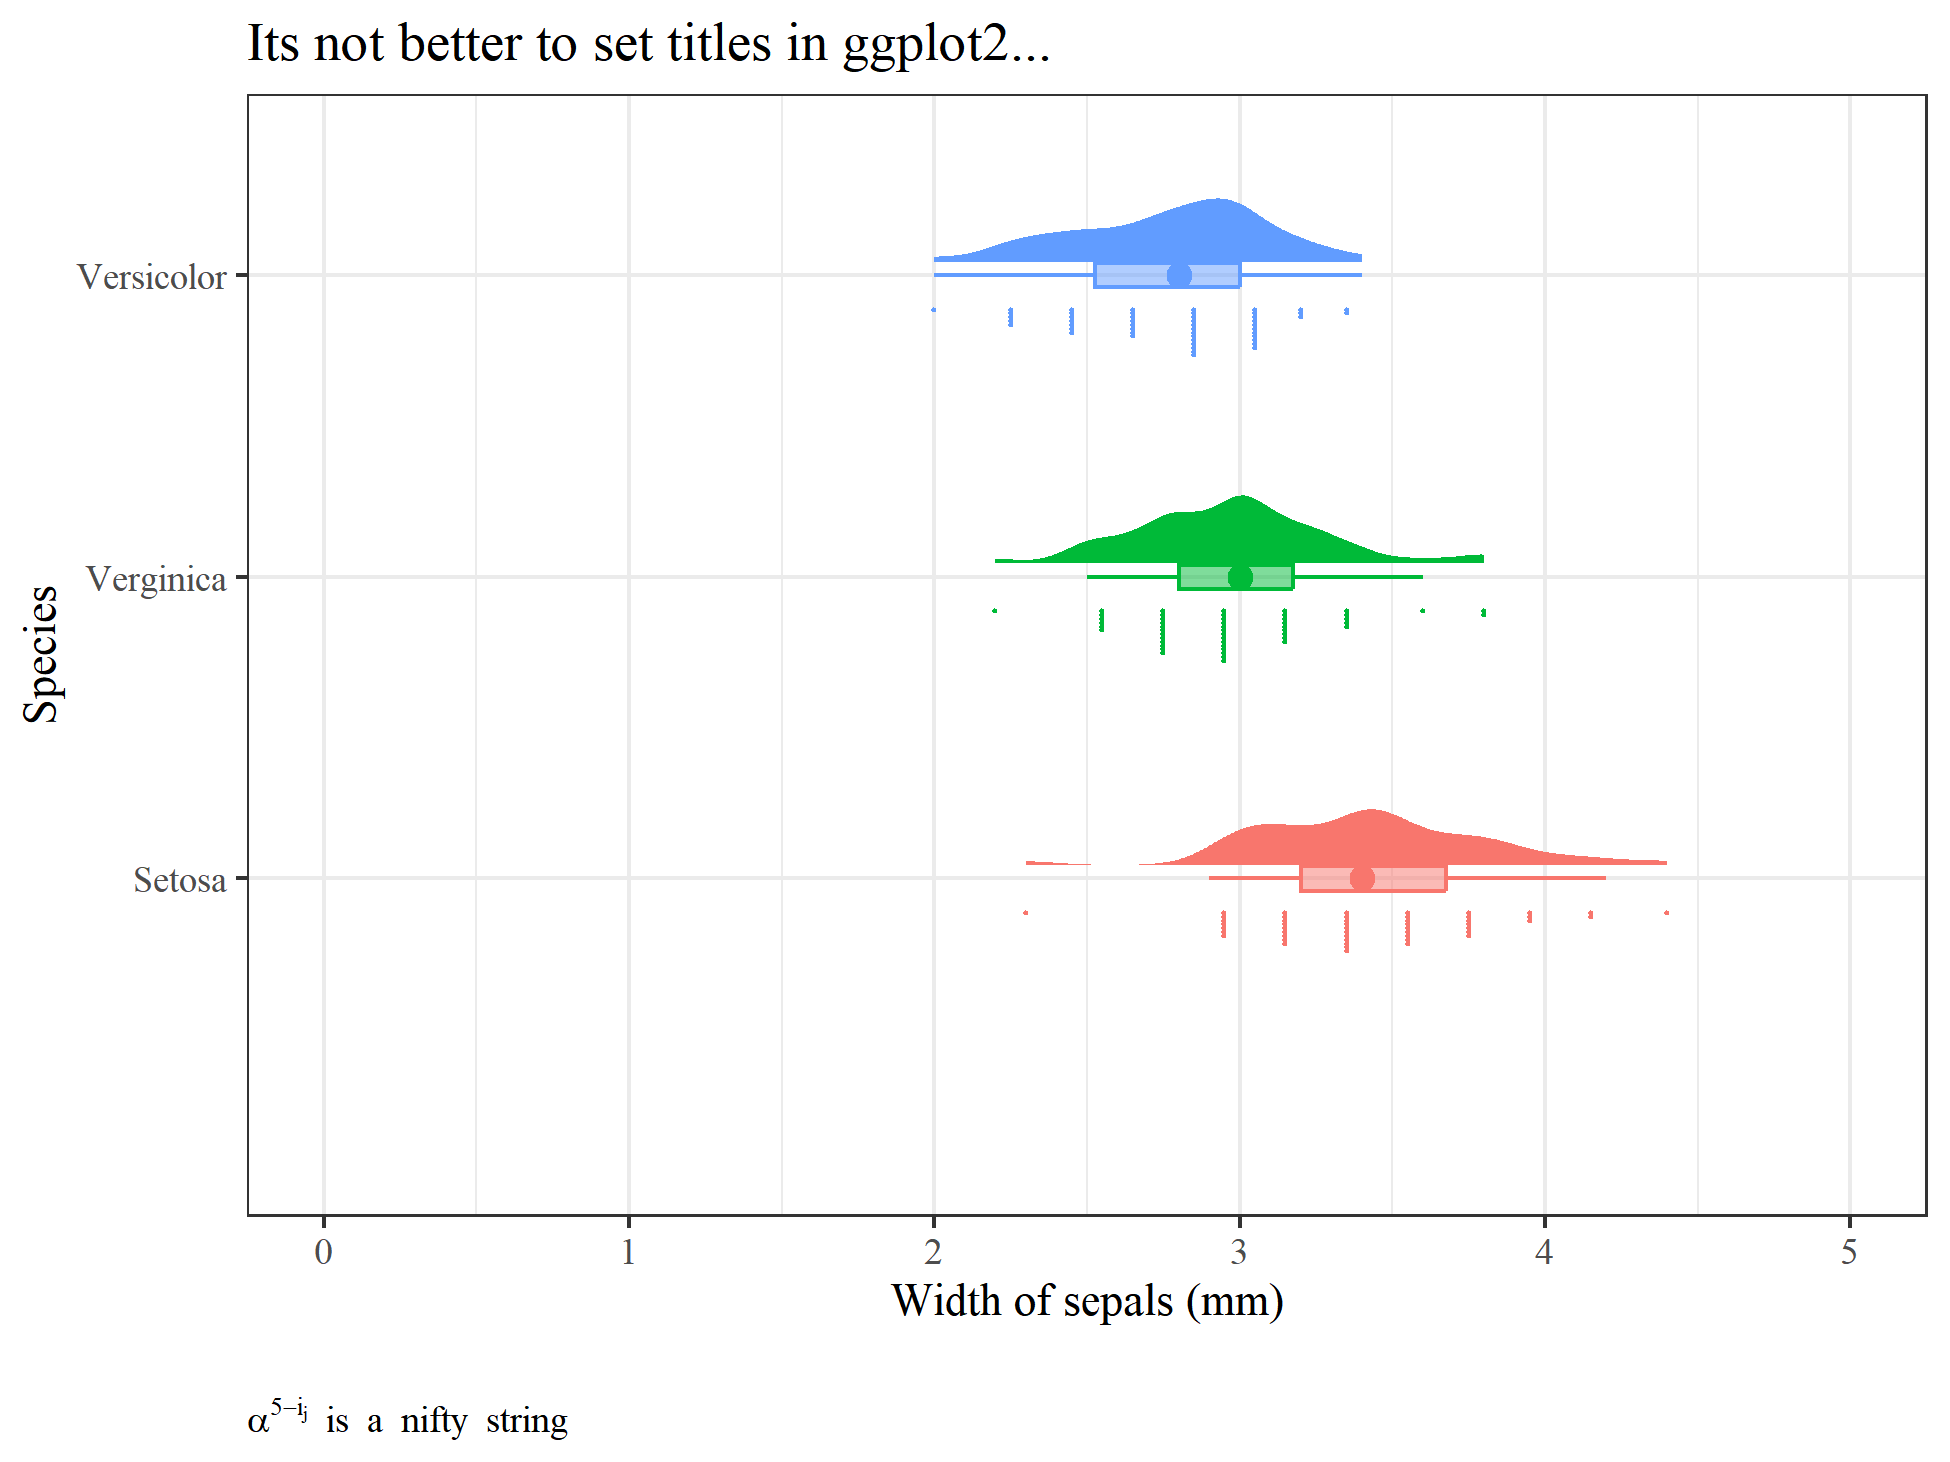
\includegraphics[width=0.9\linewidth]{cookbook_files/figure-latex/raincloud_call-1} 

}

\caption{Raincloud plot(!)}\label{fig:raincloud_call}
\end{figure}

\(~\)\\

\hypertarget{mixed-model-specification}{%
\subsubsection{Mixed model
specification}\label{mixed-model-specification}}

\(~\)\\

Lorem ipsum dolor sit amet, consectetur adipiscing elit. Maecenas et
justo non erat lobortis tincidunt. In et nunc sollicitudin, pellentesque
neque sit amet, blandit mauris. Praesent nunc urna, mattis non risus eu,
egestas bibendum nunc. Mauris et hendrerit purus. Morbi posuere nibh
erat, vel dignissim nisl fermentum sed. Vivamus nisi tellus, placerat
vitae accumsan nec, tincidunt ac leo. Phasellus sed dolor et massa
placerat sodales. Nulla facilisi. Sed sed justo nec lacus egestas
malesuada hendrerit quis ligula. Vestibulum in purus mattis, elementum
quam sit amet, eleifend lorem. Nunc dictum ligula ante, sit amet auctor
nisi aliquet non. Donec ullamcorper ultrices molestie.

Nunc sodales, massa ut vehicula auctor, augue felis faucibus urna, et
semper libero tortor accumsan magna. Proin non tortor quis erat tempor
fermentum et ut tortor. Praesent elementum tristique sapien a interdum.
Aenean sit amet mi a sapien semper ullamcorper. Phasellus quis enim
tempor, porttitor odio eu, faucibus libero. Nullam eu eros vitae eros
dictum luctus. Mauris congue ante vel laoreet eleifend.

Nunc lobortis sapien ac eros venenatis commodo. Vestibulum a venenatis
enim. Sed sit amet lectus gravida quam mollis porttitor eu ut elit.
Etiam dolor massa, dignissim et facilisis vitae, congue ac sem. Proin
sed sem condimentum, tincidunt sapien eget, accumsan dolor. Aenean
varius mi ligula, nec scelerisque ligula dignissim ac. Cras ex magna,
feugiat sed libero sed, vestibulum condimentum risus. Sed pretium
maximus est, quis imperdiet purus consectetur vestibulum. Phasellus
mattis sapien ante, convallis facilisis mi posuere quis. Maecenas id
magna scelerisque, ultrices sem viverra, ornare lectus. Ut consectetur
eleifend tortor sagittis venenatis. Cras quis lorem et odio tristique
gravida. Sed sapien justo, euismod id ligula quis, fringilla egestas
nulla. Aenean molestie felis ut aliquam scelerisque. Maecenas id ligula
ultricies, tristique sem eu, eleifend est. Cras tempor feugiat nibh sit
amet efficitur.

These are some texts.

\begin{figure}[H]
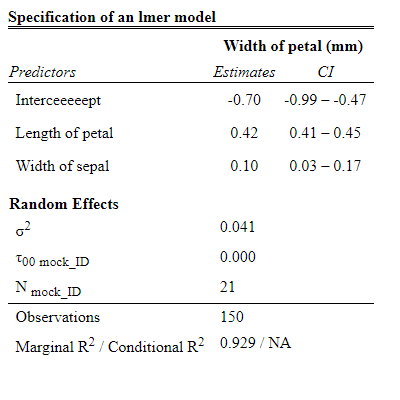
\includegraphics[width = 30em]{figure/webshot.png}
\centering
\caption{Ezt nem az R készítette}
\label{fig:webshot_sjPlot}
\end{figure}

Cashycashing\ldots.

plottyplotting\ldots{}

\begin{figure}[H]

{\centering 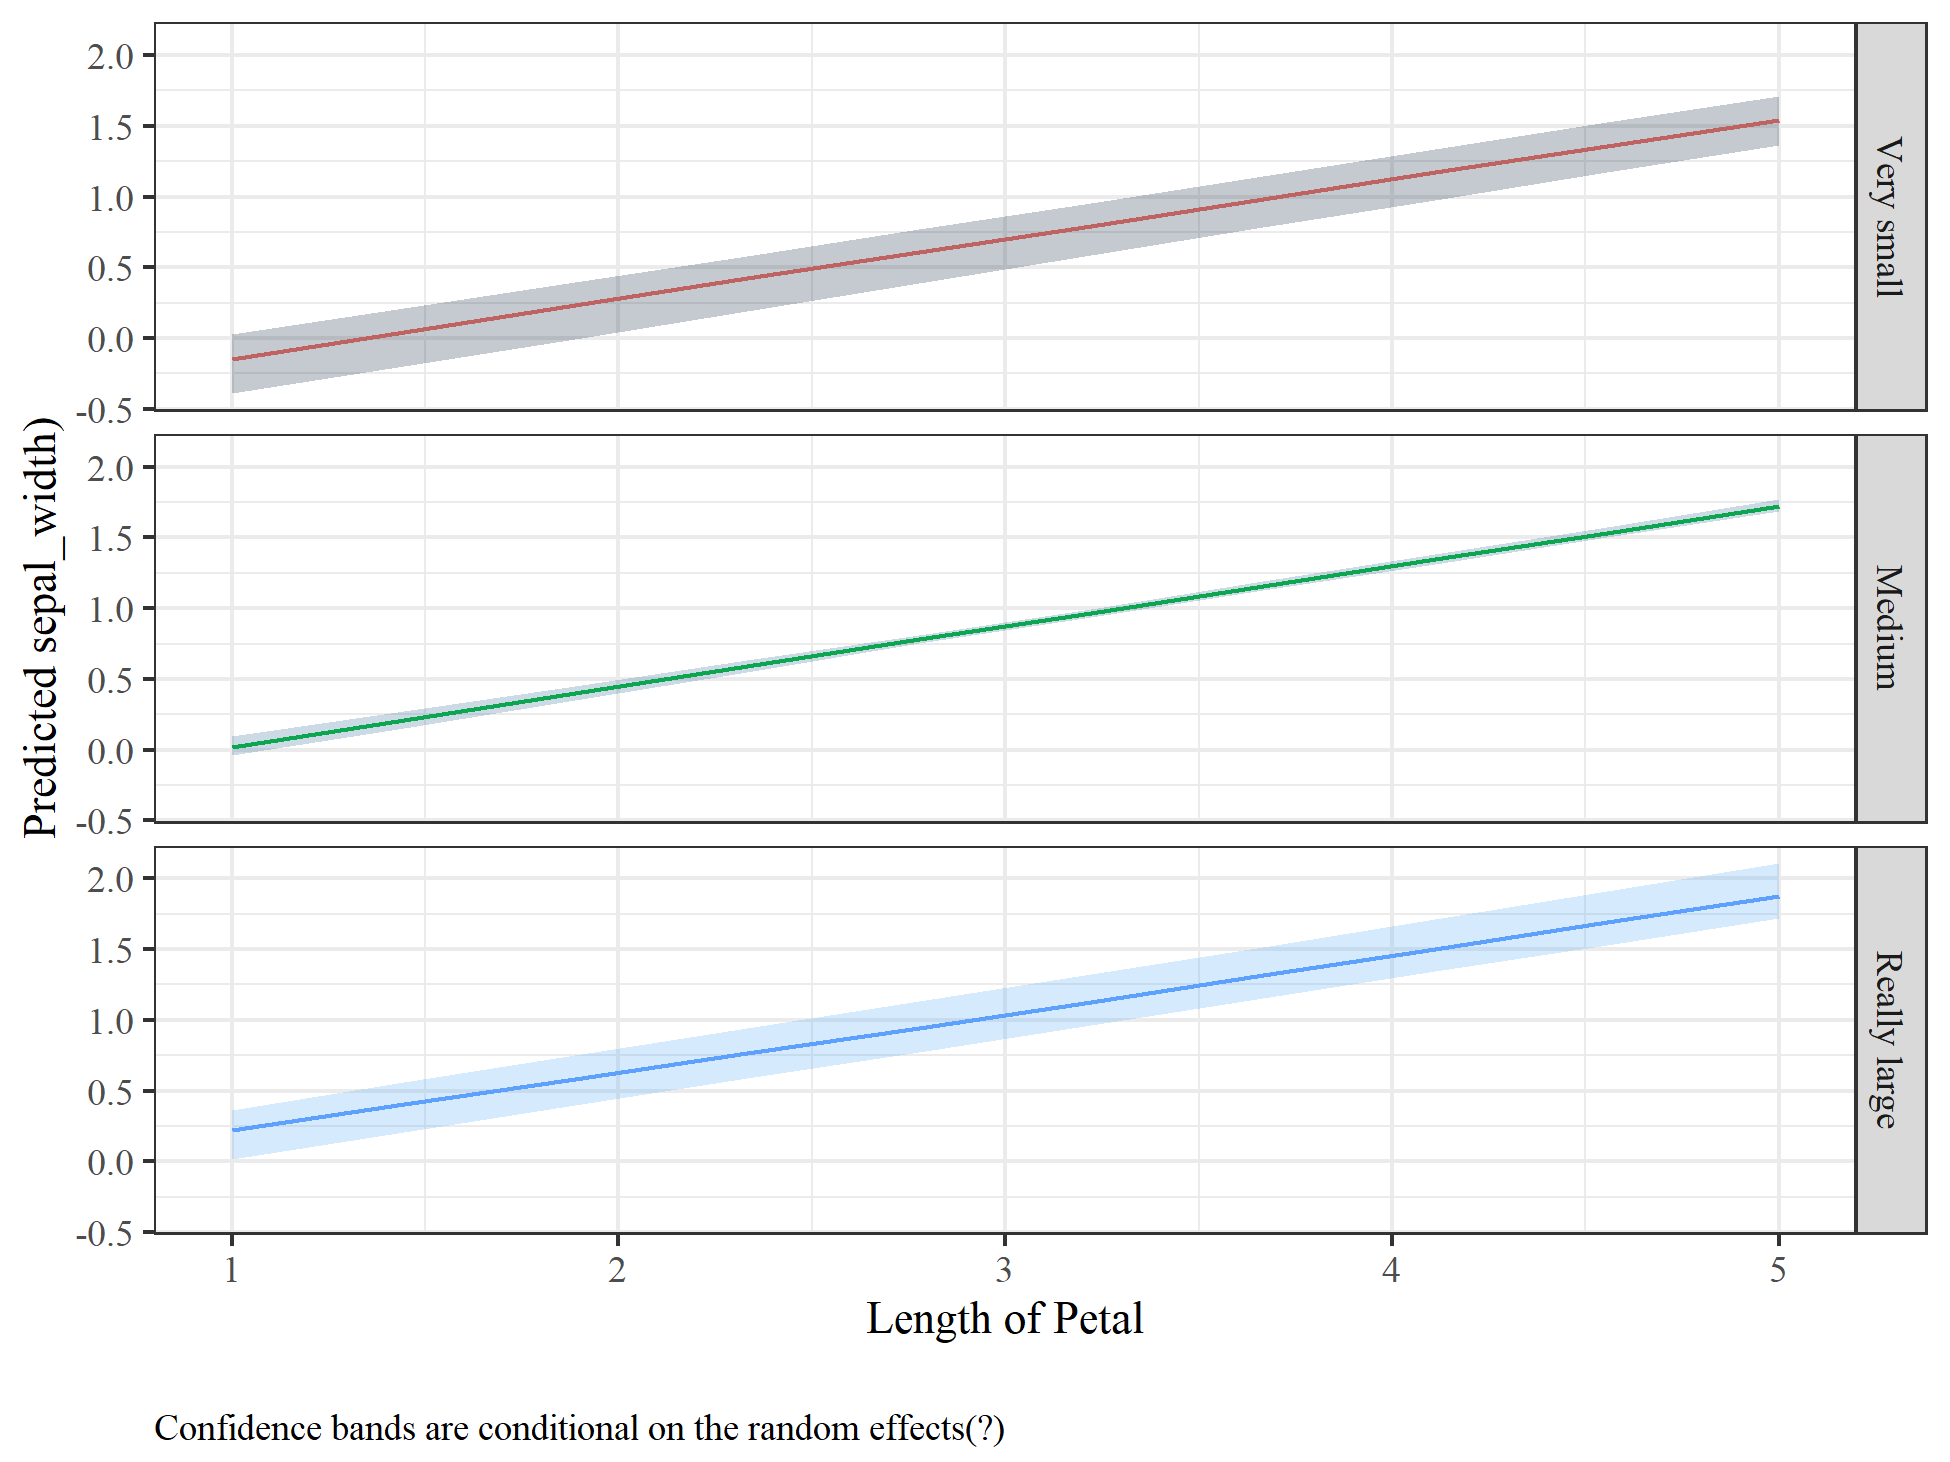
\includegraphics[width=0.9\linewidth]{cookbook_files/figure-latex/lmer_predictions-1} 

}

\caption{lmer predictions with bootstrap and labelled facets}\label{fig:lmer_predictions}
\end{figure}

\begin{figure}[H]

{\centering 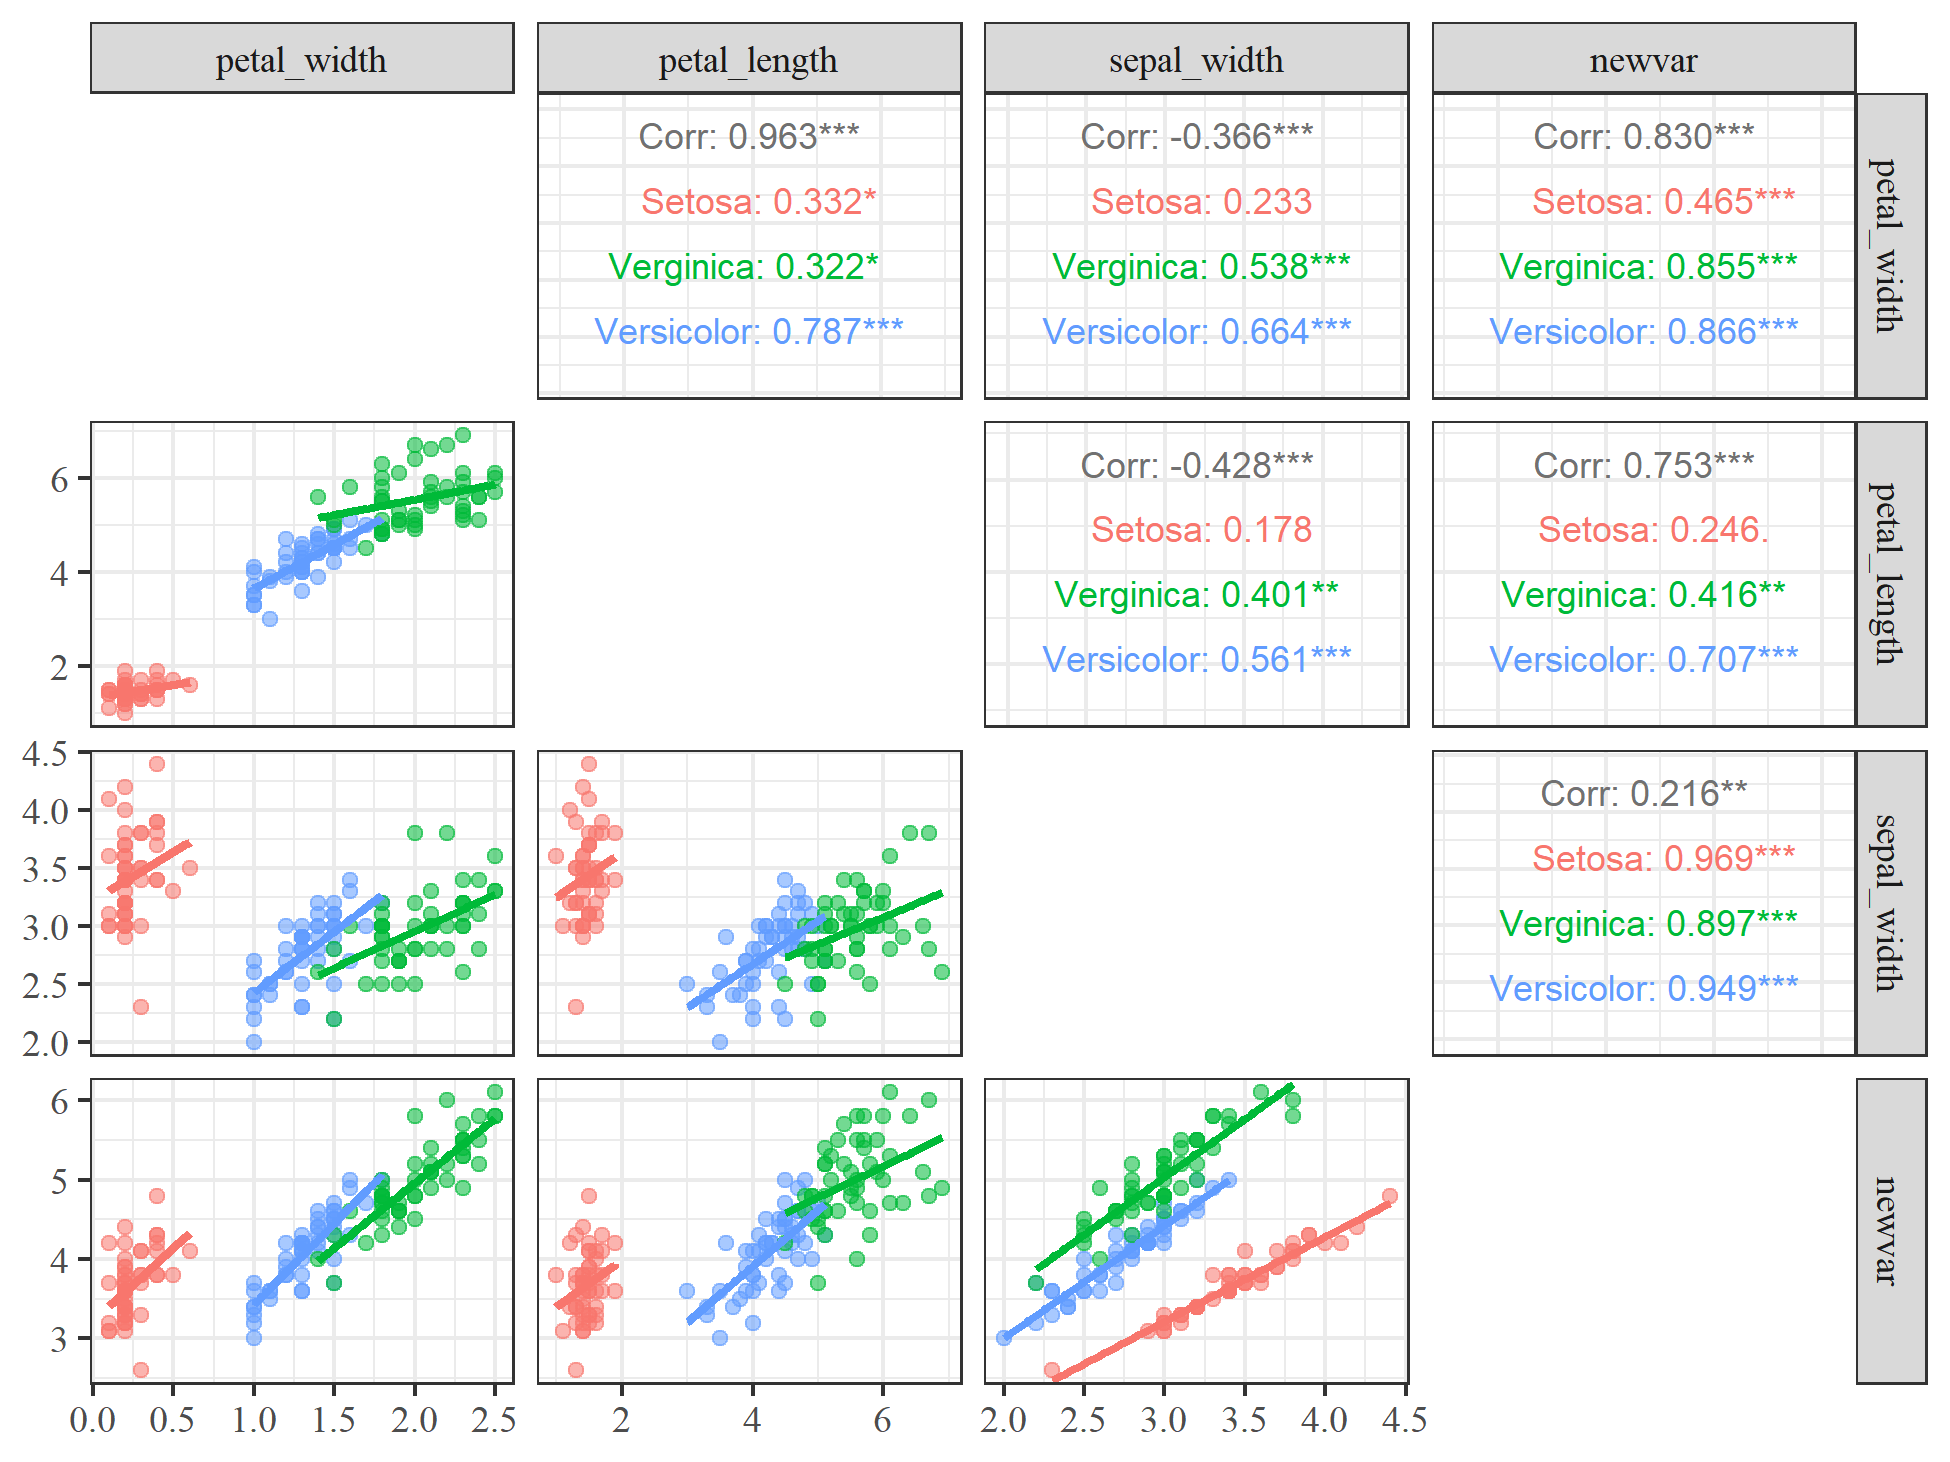
\includegraphics[width=0.9\linewidth]{cookbook_files/figure-latex/ggpairs_plot-1} 

}

\caption{Especially Cool 'pairs' plot}\label{fig:ggpairs_plot}
\end{figure}

\FloatBarrier
\newpage

\hypertarget{cyl}{%
\subsubsection{cyl}\label{cyl}}

\hypertarget{table}{%
\paragraph{Table}\label{table}}

 
  \providecommand{\huxb}[2]{\arrayrulecolor[RGB]{#1}\global\arrayrulewidth=#2pt}
  \providecommand{\huxvb}[2]{\color[RGB]{#1}\vrule width #2pt}
  \providecommand{\huxtpad}[1]{\rule{0pt}{#1}}
  \providecommand{\huxbpad}[1]{\rule[-#1]{0pt}{#1}}

\begin{table}[h]
\begin{centerbox}
\begin{threeparttable}
\captionsetup{justification=centering,singlelinecheck=off}
\caption{Frequency of cyl categories}
 \label{tab:unnamed-chunk-14}
\setlength{\tabcolsep}{0pt}
\begin{tabularx}{0.95\textwidth}{p{0.475\textwidth} p{0.475\textwidth}}


\hhline{>{\huxb{0, 0, 0}{0.8}}->{\huxb{0, 0, 0}{0.8}}-}
\arrayrulecolor{black}

\multicolumn{1}{!{\huxvb{0, 0, 0}{0.8}}m{0.475\textwidth}!{\huxvb{0, 0, 0}{0.8}}}{\cellcolor[RGB]{204, 204, 204}\hspace{6pt}\parbox[c]{0.475\textwidth-6pt-6pt}{\huxtpad{6pt + 1em}\raggedright \textbf{
}\huxbpad{6pt}}} &
\multicolumn{1}{m{0.475\textwidth}!{\huxvb{0, 0, 0}{0.8}}}{\cellcolor[RGB]{204, 204, 204}\hspace{6pt}\parbox[c]{0.475\textwidth-6pt-6pt}{\huxtpad{6pt + 1em}\centering \textbf{\textbf{N = 32}
}\huxbpad{6pt}}} \tabularnewline[-0.5pt]


\hhline{>{\huxb{0, 0, 0}{0.8}}->{\huxb{0, 0, 0}{0.8}}-}
\arrayrulecolor{black}

\multicolumn{1}{!{\huxvb{0, 0, 0}{0.8}}m{0.475\textwidth}!{\huxvb{0, 0, 0}{0.8}}}{\cellcolor[RGB]{242, 242, 242}\hspace{6pt}\parbox[c]{0.475\textwidth-6pt-6pt}{\huxtpad{6pt + 1em}\raggedright \textbf{cyl}\huxbpad{6pt}}} &
\multicolumn{1}{m{0.475\textwidth}!{\huxvb{0, 0, 0}{0.8}}}{\cellcolor[RGB]{242, 242, 242}\hspace{6pt}\parbox[c]{0.475\textwidth-6pt-6pt}{\huxtpad{6pt + 1em}\centering \huxbpad{6pt}}} \tabularnewline[-0.5pt]


\hhline{>{\huxb{0, 0, 0}{0.8}}->{\huxb{0, 0, 0}{0.8}}-}
\arrayrulecolor{black}

\multicolumn{1}{!{\huxvb{0, 0, 0}{0.8}}m{0.475\textwidth}!{\huxvb{0, 0, 0}{0.8}}}{\cellcolor[RGB]{230, 230, 230}\hspace{6pt}\parbox[c]{0.475\textwidth-6pt-6pt}{\huxtpad{6pt + 1em}\raggedright \textit{4}\huxbpad{6pt}}} &
\multicolumn{1}{m{0.475\textwidth}!{\huxvb{0, 0, 0}{0.8}}}{\cellcolor[RGB]{230, 230, 230}\hspace{6pt}\parbox[c]{0.475\textwidth-6pt-6pt}{\huxtpad{6pt + 1em}\centering 11 (34\%)\huxbpad{6pt}}} \tabularnewline[-0.5pt]


\hhline{>{\huxb{0, 0, 0}{0.8}}->{\huxb{0, 0, 0}{0.8}}-}
\arrayrulecolor{black}

\multicolumn{1}{!{\huxvb{0, 0, 0}{0.8}}m{0.475\textwidth}!{\huxvb{0, 0, 0}{0.8}}}{\cellcolor[RGB]{242, 242, 242}\hspace{6pt}\parbox[c]{0.475\textwidth-6pt-6pt}{\huxtpad{6pt + 1em}\raggedright \textit{6}\huxbpad{6pt}}} &
\multicolumn{1}{m{0.475\textwidth}!{\huxvb{0, 0, 0}{0.8}}}{\cellcolor[RGB]{242, 242, 242}\hspace{6pt}\parbox[c]{0.475\textwidth-6pt-6pt}{\huxtpad{6pt + 1em}\centering 7 (22\%)\huxbpad{6pt}}} \tabularnewline[-0.5pt]


\hhline{>{\huxb{0, 0, 0}{0.8}}->{\huxb{0, 0, 0}{0.8}}-}
\arrayrulecolor{black}

\multicolumn{1}{!{\huxvb{0, 0, 0}{0.8}}m{0.475\textwidth}!{\huxvb{0, 0, 0}{0.8}}}{\cellcolor[RGB]{230, 230, 230}\hspace{6pt}\parbox[c]{0.475\textwidth-6pt-6pt}{\huxtpad{6pt + 1em}\raggedright \textit{8}\huxbpad{6pt}}} &
\multicolumn{1}{m{0.475\textwidth}!{\huxvb{0, 0, 0}{0.8}}}{\cellcolor[RGB]{230, 230, 230}\hspace{6pt}\parbox[c]{0.475\textwidth-6pt-6pt}{\huxtpad{6pt + 1em}\centering 14 (44\%)\huxbpad{6pt}}} \tabularnewline[-0.5pt]


\hhline{>{\huxb{0, 0, 0}{0.8}}->{\huxb{0, 0, 0}{0.8}}-}
\arrayrulecolor{black}
\end{tabularx}
\end{threeparttable}\par\end{centerbox}

\end{table}
 

\hypertarget{figures}{%
\paragraph{Figures}\label{figures}}

\begin{figure}[h]
\begin{multicols}{2}
\begin{figure}[H]
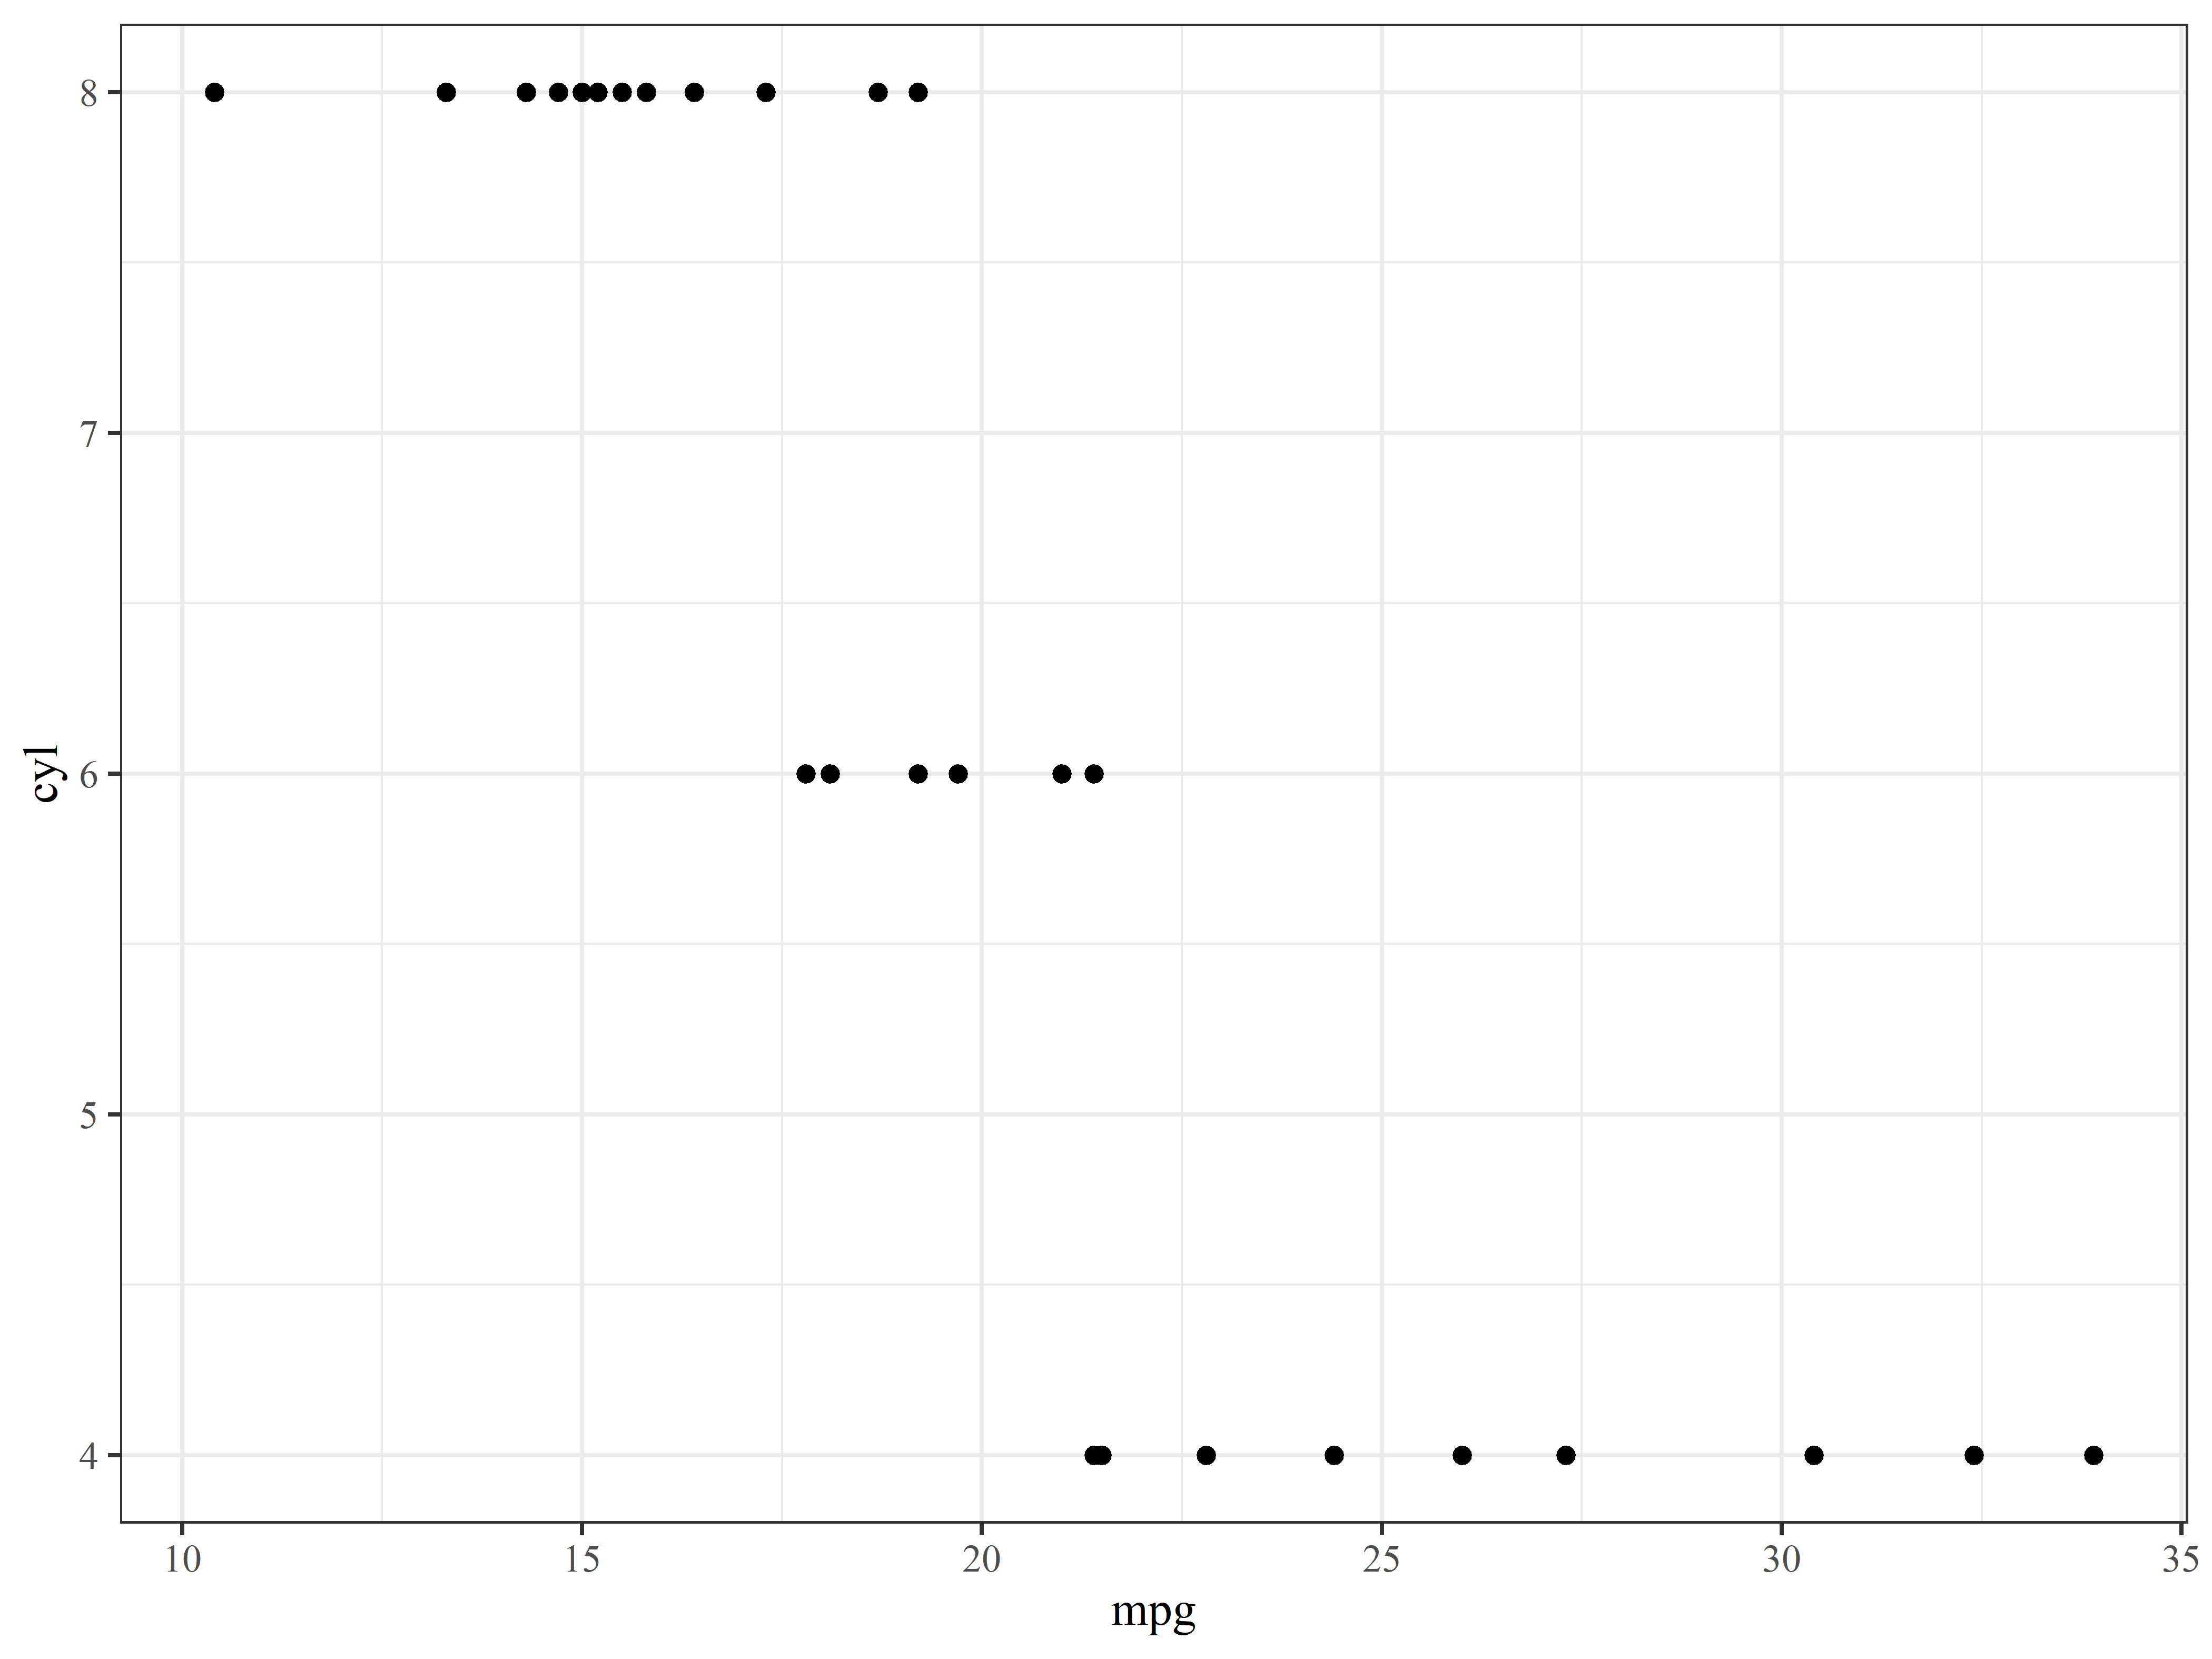
\includegraphics[width = \linewidth]{cookbook_files/figure-latex/cyl-fig1-1}
\caption{Bal oldali ábra}
\label{fig:bar2_a2}
\end{figure}

\columnbreak

\begin{figure}[H]
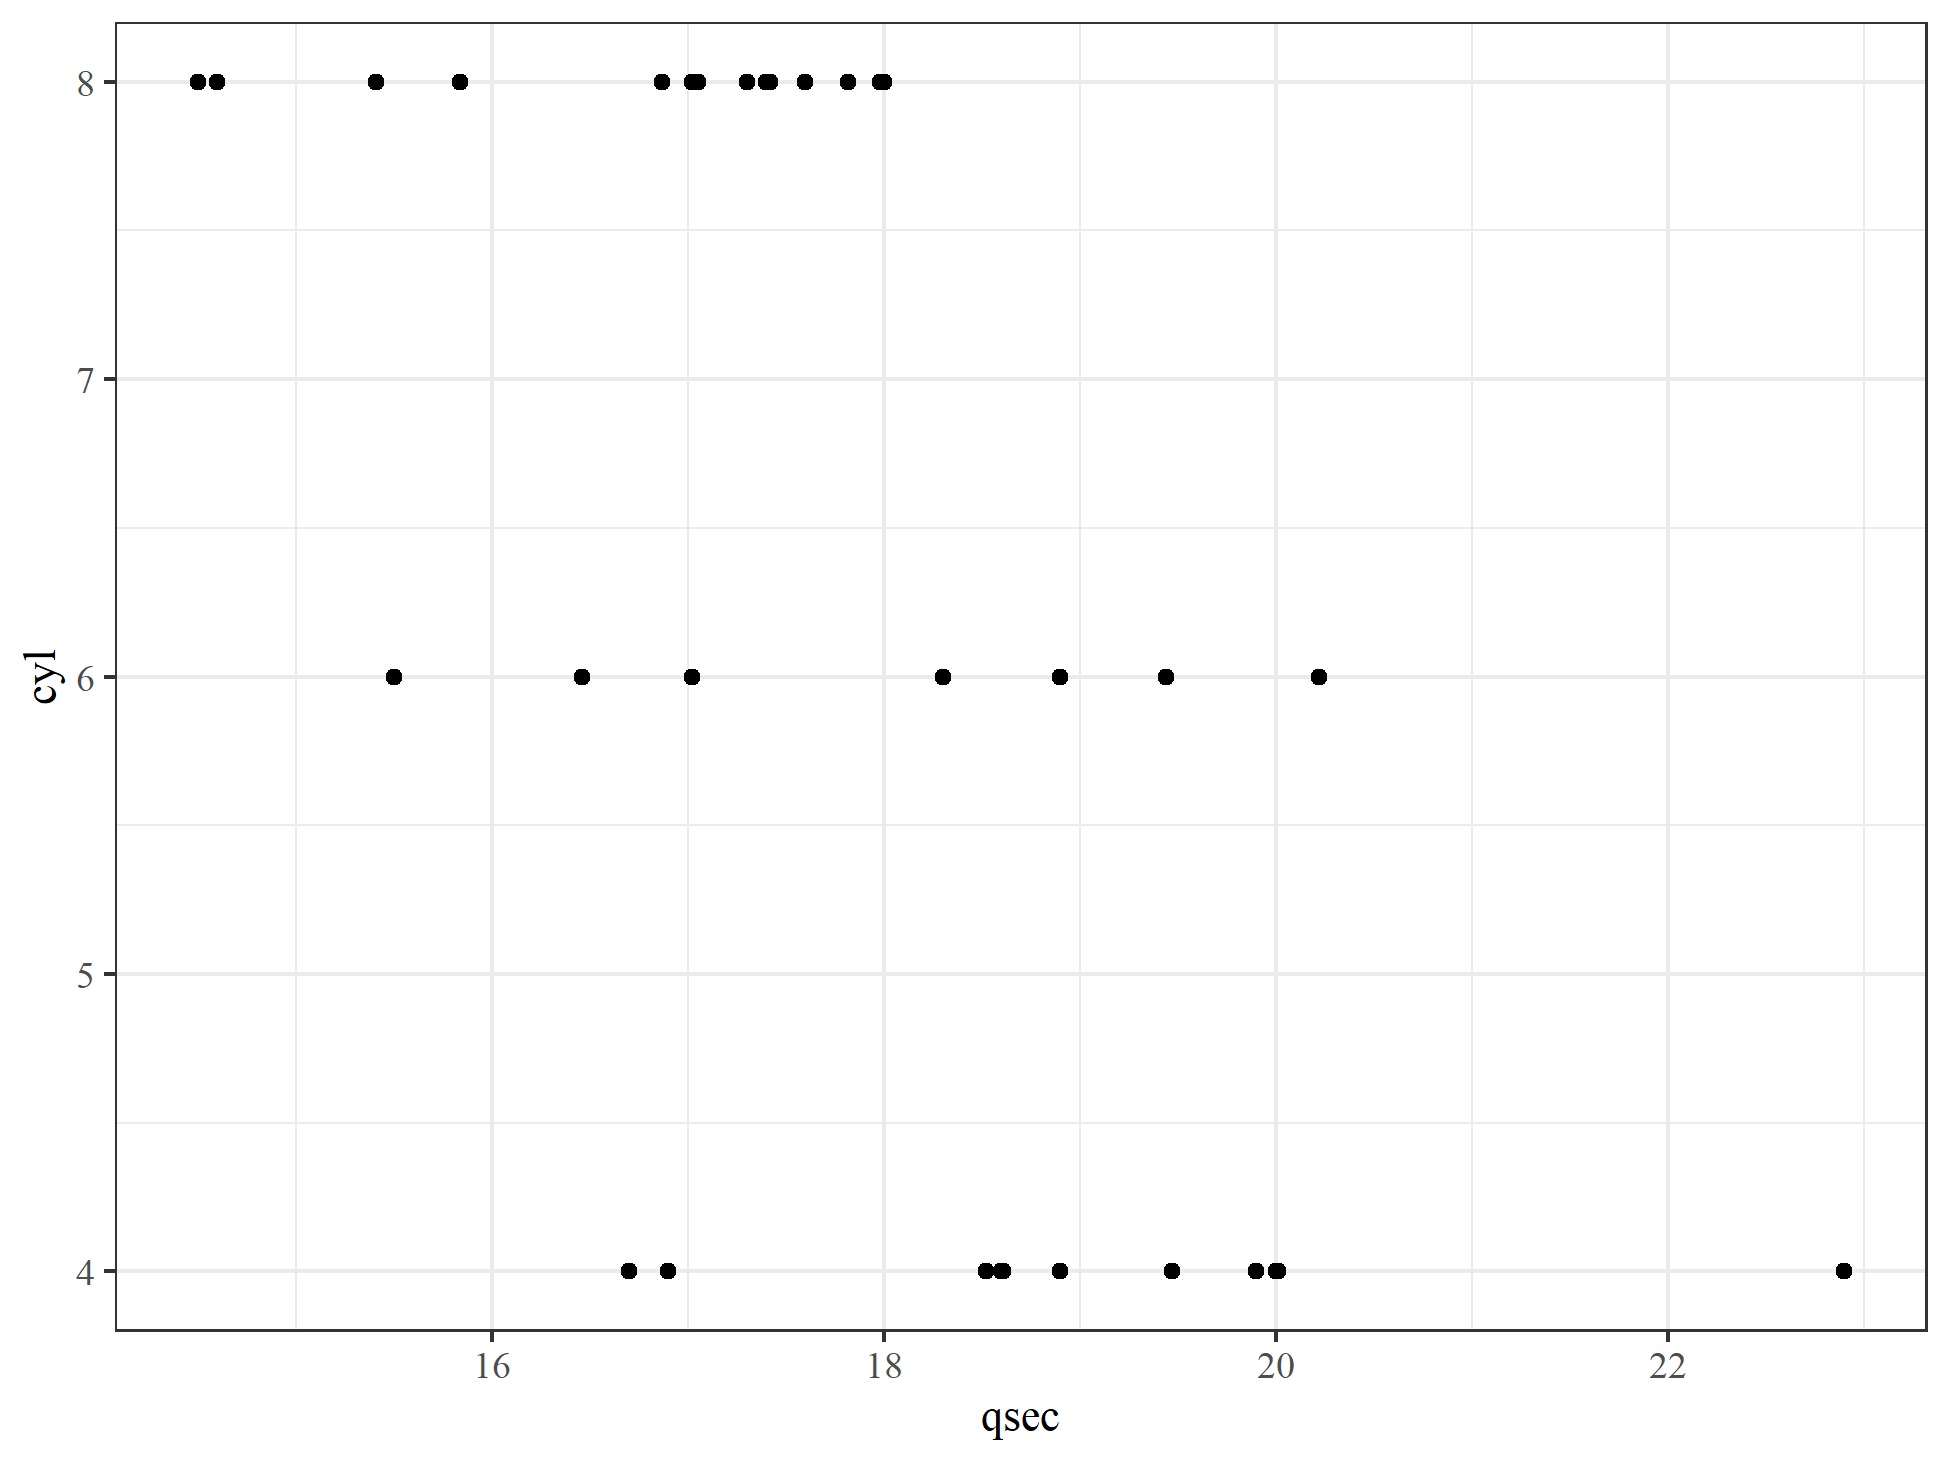
\includegraphics[width = \linewidth]{cookbook_files/figure-latex/cyl-fig1-2}
\centering
\caption{Jobb oldali ábra}
\label{fig:bar2_b2}
\end{figure}
\end{multicols}
\end{figure}

És még hivatkozni is tudunk a(z) \ref{fig:param_plot12}. ábrára.

\hypertarget{gear}{%
\subsubsection{gear}\label{gear}}

\hypertarget{table-1}{%
\paragraph{Table}\label{table-1}}

 
  \providecommand{\huxb}[2]{\arrayrulecolor[RGB]{#1}\global\arrayrulewidth=#2pt}
  \providecommand{\huxvb}[2]{\color[RGB]{#1}\vrule width #2pt}
  \providecommand{\huxtpad}[1]{\rule{0pt}{#1}}
  \providecommand{\huxbpad}[1]{\rule[-#1]{0pt}{#1}}

\begin{table}[h]
\begin{centerbox}
\begin{threeparttable}
\captionsetup{justification=centering,singlelinecheck=off}
\caption{Frequency of gear categories}
 \label{tab:unnamed-chunk-18}
\setlength{\tabcolsep}{0pt}
\begin{tabularx}{0.95\textwidth}{p{0.475\textwidth} p{0.475\textwidth}}


\hhline{>{\huxb{0, 0, 0}{0.8}}->{\huxb{0, 0, 0}{0.8}}-}
\arrayrulecolor{black}

\multicolumn{1}{!{\huxvb{0, 0, 0}{0.8}}m{0.475\textwidth}!{\huxvb{0, 0, 0}{0.8}}}{\cellcolor[RGB]{204, 204, 204}\hspace{6pt}\parbox[c]{0.475\textwidth-6pt-6pt}{\huxtpad{6pt + 1em}\raggedright \textbf{
}\huxbpad{6pt}}} &
\multicolumn{1}{m{0.475\textwidth}!{\huxvb{0, 0, 0}{0.8}}}{\cellcolor[RGB]{204, 204, 204}\hspace{6pt}\parbox[c]{0.475\textwidth-6pt-6pt}{\huxtpad{6pt + 1em}\centering \textbf{\textbf{N = 32}
}\huxbpad{6pt}}} \tabularnewline[-0.5pt]


\hhline{>{\huxb{0, 0, 0}{0.8}}->{\huxb{0, 0, 0}{0.8}}-}
\arrayrulecolor{black}

\multicolumn{1}{!{\huxvb{0, 0, 0}{0.8}}m{0.475\textwidth}!{\huxvb{0, 0, 0}{0.8}}}{\cellcolor[RGB]{242, 242, 242}\hspace{6pt}\parbox[c]{0.475\textwidth-6pt-6pt}{\huxtpad{6pt + 1em}\raggedright \textbf{gear}\huxbpad{6pt}}} &
\multicolumn{1}{m{0.475\textwidth}!{\huxvb{0, 0, 0}{0.8}}}{\cellcolor[RGB]{242, 242, 242}\hspace{6pt}\parbox[c]{0.475\textwidth-6pt-6pt}{\huxtpad{6pt + 1em}\centering \huxbpad{6pt}}} \tabularnewline[-0.5pt]


\hhline{>{\huxb{0, 0, 0}{0.8}}->{\huxb{0, 0, 0}{0.8}}-}
\arrayrulecolor{black}

\multicolumn{1}{!{\huxvb{0, 0, 0}{0.8}}m{0.475\textwidth}!{\huxvb{0, 0, 0}{0.8}}}{\cellcolor[RGB]{230, 230, 230}\hspace{6pt}\parbox[c]{0.475\textwidth-6pt-6pt}{\huxtpad{6pt + 1em}\raggedright \textit{3}\huxbpad{6pt}}} &
\multicolumn{1}{m{0.475\textwidth}!{\huxvb{0, 0, 0}{0.8}}}{\cellcolor[RGB]{230, 230, 230}\hspace{6pt}\parbox[c]{0.475\textwidth-6pt-6pt}{\huxtpad{6pt + 1em}\centering 15 (47\%)\huxbpad{6pt}}} \tabularnewline[-0.5pt]


\hhline{>{\huxb{0, 0, 0}{0.8}}->{\huxb{0, 0, 0}{0.8}}-}
\arrayrulecolor{black}

\multicolumn{1}{!{\huxvb{0, 0, 0}{0.8}}m{0.475\textwidth}!{\huxvb{0, 0, 0}{0.8}}}{\cellcolor[RGB]{242, 242, 242}\hspace{6pt}\parbox[c]{0.475\textwidth-6pt-6pt}{\huxtpad{6pt + 1em}\raggedright \textit{4}\huxbpad{6pt}}} &
\multicolumn{1}{m{0.475\textwidth}!{\huxvb{0, 0, 0}{0.8}}}{\cellcolor[RGB]{242, 242, 242}\hspace{6pt}\parbox[c]{0.475\textwidth-6pt-6pt}{\huxtpad{6pt + 1em}\centering 12 (38\%)\huxbpad{6pt}}} \tabularnewline[-0.5pt]


\hhline{>{\huxb{0, 0, 0}{0.8}}->{\huxb{0, 0, 0}{0.8}}-}
\arrayrulecolor{black}

\multicolumn{1}{!{\huxvb{0, 0, 0}{0.8}}m{0.475\textwidth}!{\huxvb{0, 0, 0}{0.8}}}{\cellcolor[RGB]{230, 230, 230}\hspace{6pt}\parbox[c]{0.475\textwidth-6pt-6pt}{\huxtpad{6pt + 1em}\raggedright \textit{5}\huxbpad{6pt}}} &
\multicolumn{1}{m{0.475\textwidth}!{\huxvb{0, 0, 0}{0.8}}}{\cellcolor[RGB]{230, 230, 230}\hspace{6pt}\parbox[c]{0.475\textwidth-6pt-6pt}{\huxtpad{6pt + 1em}\centering 5 (16\%)\huxbpad{6pt}}} \tabularnewline[-0.5pt]


\hhline{>{\huxb{0, 0, 0}{0.8}}->{\huxb{0, 0, 0}{0.8}}-}
\arrayrulecolor{black}
\end{tabularx}
\end{threeparttable}\par\end{centerbox}

\end{table}
 

\hypertarget{figures-1}{%
\paragraph{Figures}\label{figures-1}}

\begin{figure}[h]
\begin{multicols}{2}
\begin{figure}[H]
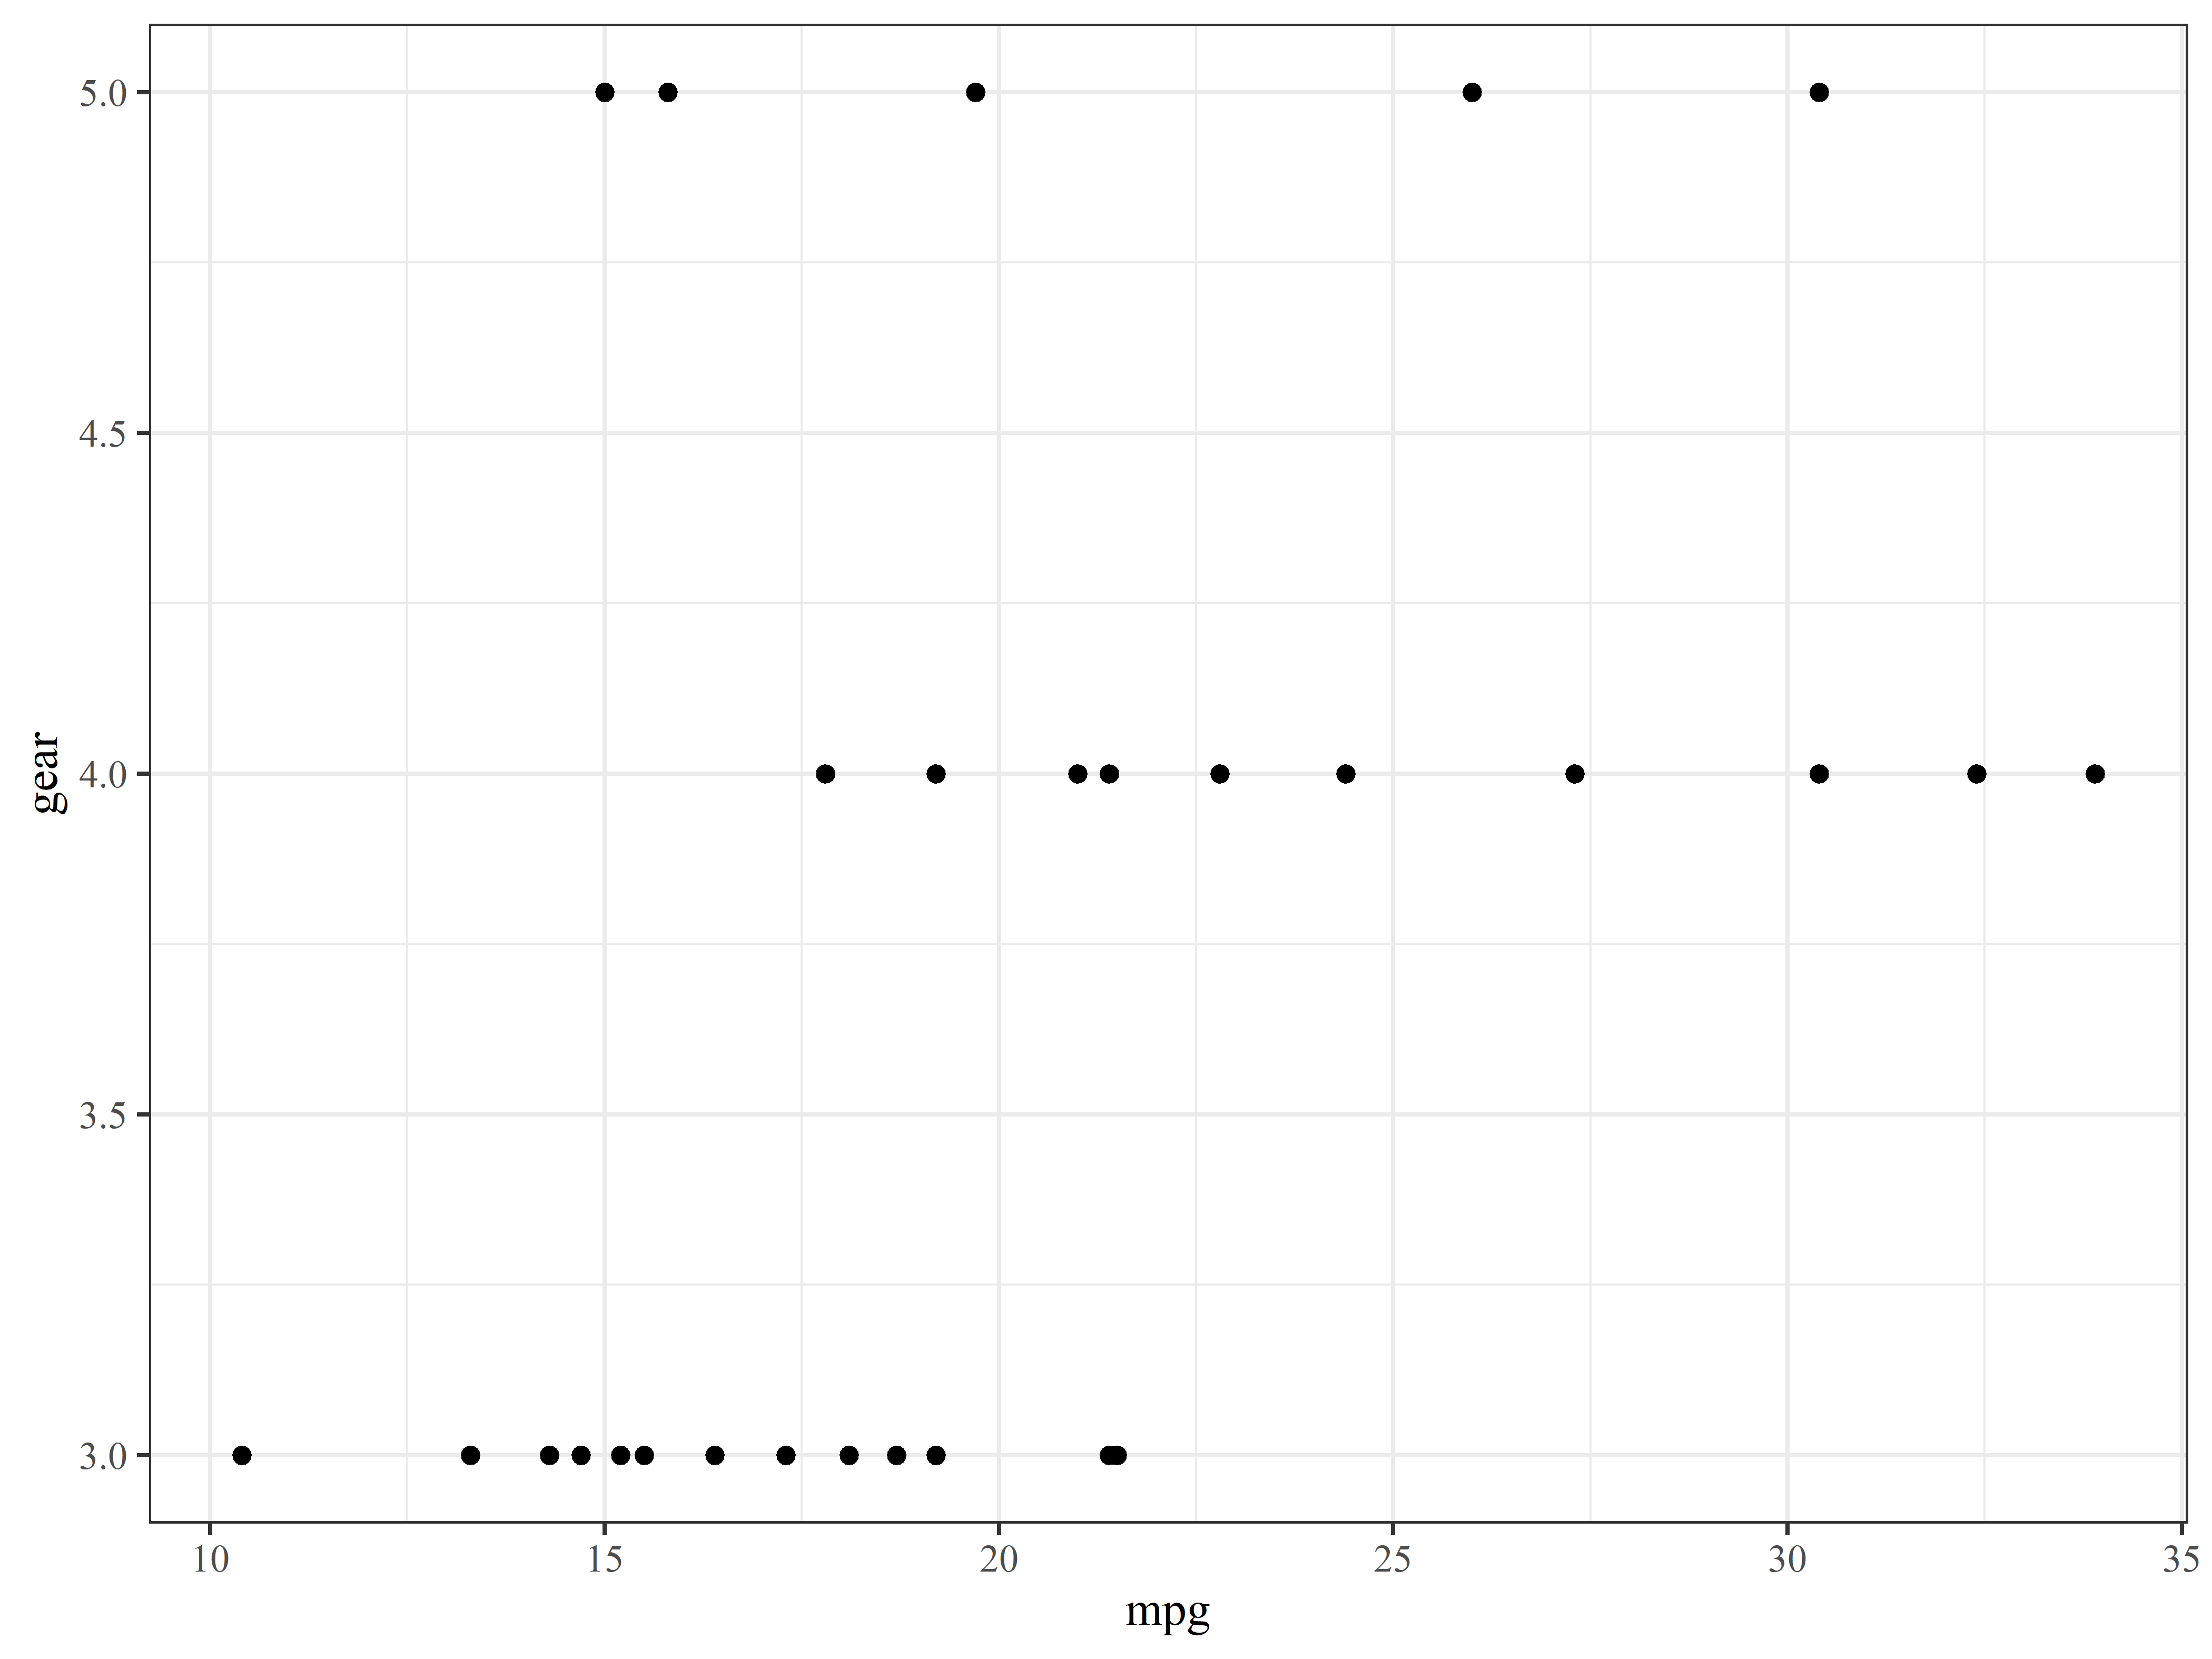
\includegraphics[width = \linewidth]{cookbook_files/figure-latex/gear-fig1-1}
\caption{Bal oldali ábra}
\label{fig:bar2_a4}
\end{figure}

\columnbreak

\begin{figure}[H]
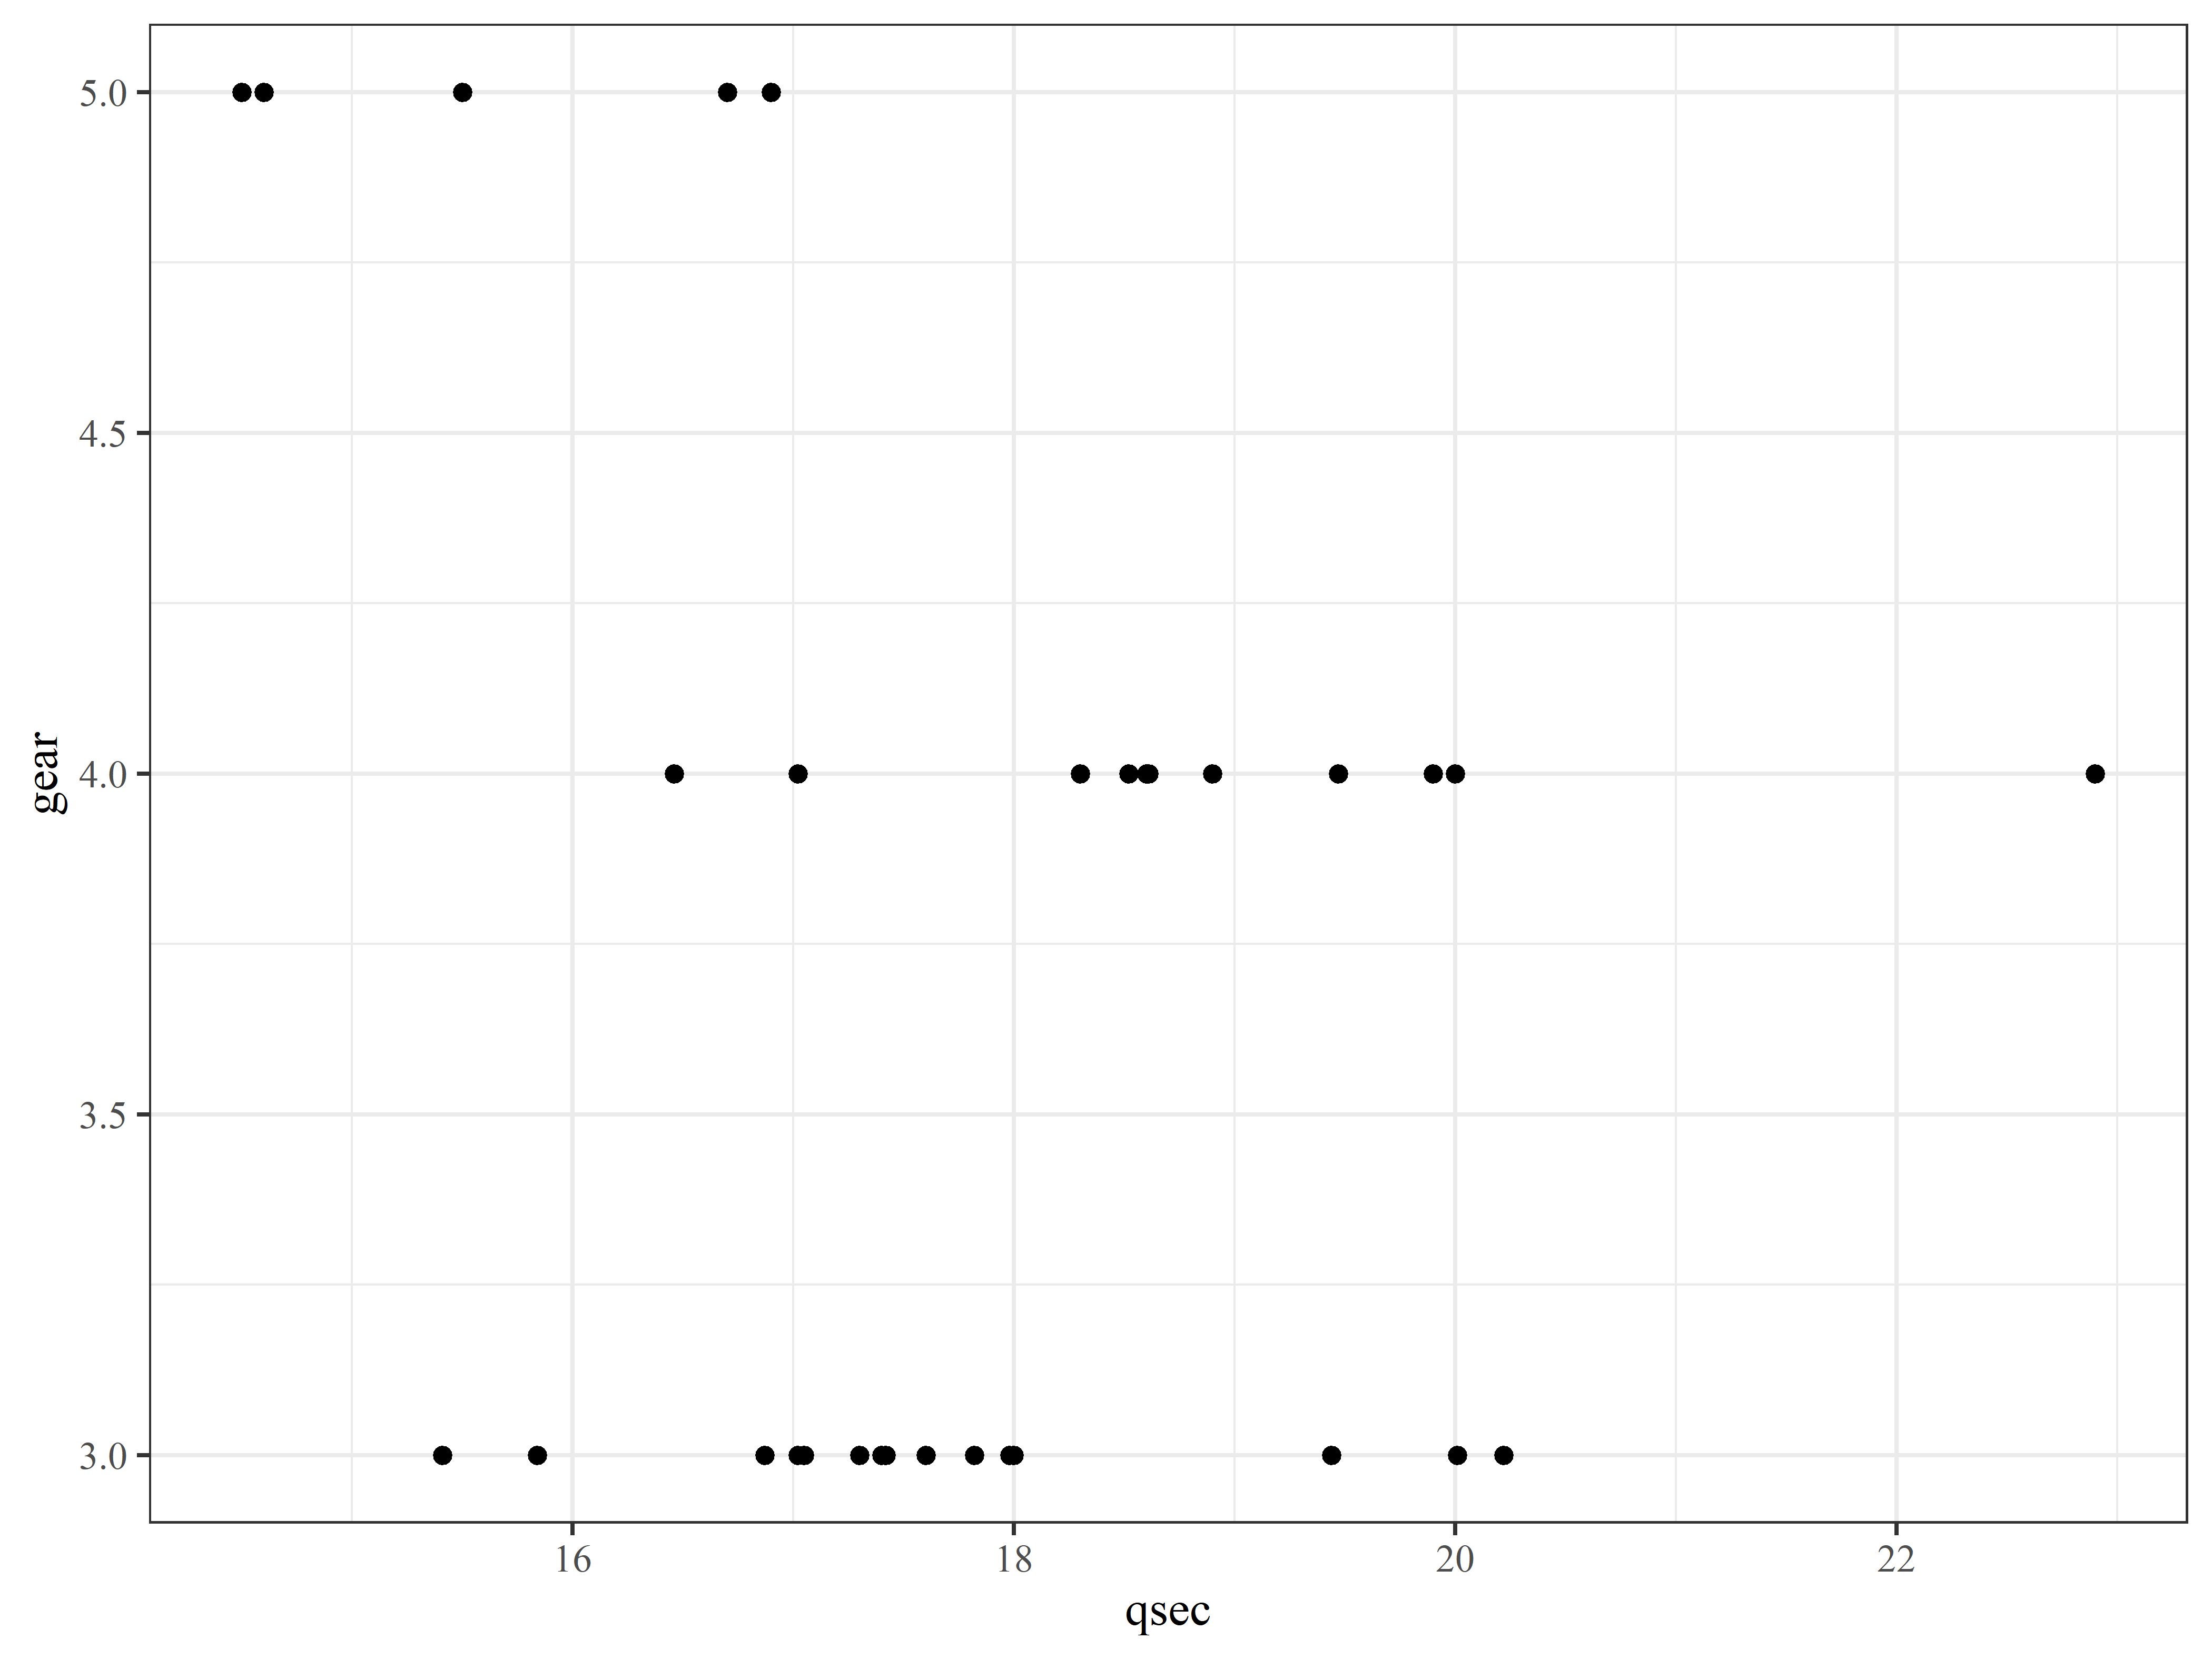
\includegraphics[width = \linewidth]{cookbook_files/figure-latex/gear-fig1-2}
\centering
\caption{Jobb oldali ábra}
\label{fig:bar2_b4}
\end{figure}
\end{multicols}
\end{figure}

És még hivatkozni is tudunk a(z) \ref{fig:param_plot14}. ábrára.

\hypertarget{carb}{%
\subsubsection{carb}\label{carb}}

\hypertarget{table-2}{%
\paragraph{Table}\label{table-2}}

 
  \providecommand{\huxb}[2]{\arrayrulecolor[RGB]{#1}\global\arrayrulewidth=#2pt}
  \providecommand{\huxvb}[2]{\color[RGB]{#1}\vrule width #2pt}
  \providecommand{\huxtpad}[1]{\rule{0pt}{#1}}
  \providecommand{\huxbpad}[1]{\rule[-#1]{0pt}{#1}}

\begin{table}[h]
\begin{centerbox}
\begin{threeparttable}
\captionsetup{justification=centering,singlelinecheck=off}
\caption{Frequency of carb categories}
 \label{tab:unnamed-chunk-22}
\setlength{\tabcolsep}{0pt}
\begin{tabularx}{0.95\textwidth}{p{0.475\textwidth} p{0.475\textwidth}}


\hhline{>{\huxb{0, 0, 0}{0.8}}->{\huxb{0, 0, 0}{0.8}}-}
\arrayrulecolor{black}

\multicolumn{1}{!{\huxvb{0, 0, 0}{0.8}}m{0.475\textwidth}!{\huxvb{0, 0, 0}{0.8}}}{\cellcolor[RGB]{204, 204, 204}\hspace{6pt}\parbox[c]{0.475\textwidth-6pt-6pt}{\huxtpad{6pt + 1em}\raggedright \textbf{
}\huxbpad{6pt}}} &
\multicolumn{1}{m{0.475\textwidth}!{\huxvb{0, 0, 0}{0.8}}}{\cellcolor[RGB]{204, 204, 204}\hspace{6pt}\parbox[c]{0.475\textwidth-6pt-6pt}{\huxtpad{6pt + 1em}\centering \textbf{\textbf{N = 32}
}\huxbpad{6pt}}} \tabularnewline[-0.5pt]


\hhline{>{\huxb{0, 0, 0}{0.8}}->{\huxb{0, 0, 0}{0.8}}-}
\arrayrulecolor{black}

\multicolumn{1}{!{\huxvb{0, 0, 0}{0.8}}m{0.475\textwidth}!{\huxvb{0, 0, 0}{0.8}}}{\cellcolor[RGB]{242, 242, 242}\hspace{6pt}\parbox[c]{0.475\textwidth-6pt-6pt}{\huxtpad{6pt + 1em}\raggedright \textbf{carb}\huxbpad{6pt}}} &
\multicolumn{1}{m{0.475\textwidth}!{\huxvb{0, 0, 0}{0.8}}}{\cellcolor[RGB]{242, 242, 242}\hspace{6pt}\parbox[c]{0.475\textwidth-6pt-6pt}{\huxtpad{6pt + 1em}\centering \huxbpad{6pt}}} \tabularnewline[-0.5pt]


\hhline{>{\huxb{0, 0, 0}{0.8}}->{\huxb{0, 0, 0}{0.8}}-}
\arrayrulecolor{black}

\multicolumn{1}{!{\huxvb{0, 0, 0}{0.8}}m{0.475\textwidth}!{\huxvb{0, 0, 0}{0.8}}}{\cellcolor[RGB]{230, 230, 230}\hspace{6pt}\parbox[c]{0.475\textwidth-6pt-6pt}{\huxtpad{6pt + 1em}\raggedright \textit{1}\huxbpad{6pt}}} &
\multicolumn{1}{m{0.475\textwidth}!{\huxvb{0, 0, 0}{0.8}}}{\cellcolor[RGB]{230, 230, 230}\hspace{6pt}\parbox[c]{0.475\textwidth-6pt-6pt}{\huxtpad{6pt + 1em}\centering 7 (22\%)\huxbpad{6pt}}} \tabularnewline[-0.5pt]


\hhline{>{\huxb{0, 0, 0}{0.8}}->{\huxb{0, 0, 0}{0.8}}-}
\arrayrulecolor{black}

\multicolumn{1}{!{\huxvb{0, 0, 0}{0.8}}m{0.475\textwidth}!{\huxvb{0, 0, 0}{0.8}}}{\cellcolor[RGB]{242, 242, 242}\hspace{6pt}\parbox[c]{0.475\textwidth-6pt-6pt}{\huxtpad{6pt + 1em}\raggedright \textit{2}\huxbpad{6pt}}} &
\multicolumn{1}{m{0.475\textwidth}!{\huxvb{0, 0, 0}{0.8}}}{\cellcolor[RGB]{242, 242, 242}\hspace{6pt}\parbox[c]{0.475\textwidth-6pt-6pt}{\huxtpad{6pt + 1em}\centering 10 (31\%)\huxbpad{6pt}}} \tabularnewline[-0.5pt]


\hhline{>{\huxb{0, 0, 0}{0.8}}->{\huxb{0, 0, 0}{0.8}}-}
\arrayrulecolor{black}

\multicolumn{1}{!{\huxvb{0, 0, 0}{0.8}}m{0.475\textwidth}!{\huxvb{0, 0, 0}{0.8}}}{\cellcolor[RGB]{230, 230, 230}\hspace{6pt}\parbox[c]{0.475\textwidth-6pt-6pt}{\huxtpad{6pt + 1em}\raggedright \textit{3}\huxbpad{6pt}}} &
\multicolumn{1}{m{0.475\textwidth}!{\huxvb{0, 0, 0}{0.8}}}{\cellcolor[RGB]{230, 230, 230}\hspace{6pt}\parbox[c]{0.475\textwidth-6pt-6pt}{\huxtpad{6pt + 1em}\centering 3 (9.4\%)\huxbpad{6pt}}} \tabularnewline[-0.5pt]


\hhline{>{\huxb{0, 0, 0}{0.8}}->{\huxb{0, 0, 0}{0.8}}-}
\arrayrulecolor{black}

\multicolumn{1}{!{\huxvb{0, 0, 0}{0.8}}m{0.475\textwidth}!{\huxvb{0, 0, 0}{0.8}}}{\cellcolor[RGB]{242, 242, 242}\hspace{6pt}\parbox[c]{0.475\textwidth-6pt-6pt}{\huxtpad{6pt + 1em}\raggedright \textit{4}\huxbpad{6pt}}} &
\multicolumn{1}{m{0.475\textwidth}!{\huxvb{0, 0, 0}{0.8}}}{\cellcolor[RGB]{242, 242, 242}\hspace{6pt}\parbox[c]{0.475\textwidth-6pt-6pt}{\huxtpad{6pt + 1em}\centering 10 (31\%)\huxbpad{6pt}}} \tabularnewline[-0.5pt]


\hhline{>{\huxb{0, 0, 0}{0.8}}->{\huxb{0, 0, 0}{0.8}}-}
\arrayrulecolor{black}

\multicolumn{1}{!{\huxvb{0, 0, 0}{0.8}}m{0.475\textwidth}!{\huxvb{0, 0, 0}{0.8}}}{\cellcolor[RGB]{230, 230, 230}\hspace{6pt}\parbox[c]{0.475\textwidth-6pt-6pt}{\huxtpad{6pt + 1em}\raggedright \textit{6}\huxbpad{6pt}}} &
\multicolumn{1}{m{0.475\textwidth}!{\huxvb{0, 0, 0}{0.8}}}{\cellcolor[RGB]{230, 230, 230}\hspace{6pt}\parbox[c]{0.475\textwidth-6pt-6pt}{\huxtpad{6pt + 1em}\centering 1 (3.1\%)\huxbpad{6pt}}} \tabularnewline[-0.5pt]


\hhline{>{\huxb{0, 0, 0}{0.8}}->{\huxb{0, 0, 0}{0.8}}-}
\arrayrulecolor{black}

\multicolumn{1}{!{\huxvb{0, 0, 0}{0.8}}m{0.475\textwidth}!{\huxvb{0, 0, 0}{0.8}}}{\cellcolor[RGB]{242, 242, 242}\hspace{6pt}\parbox[c]{0.475\textwidth-6pt-6pt}{\huxtpad{6pt + 1em}\raggedright \textit{8}\huxbpad{6pt}}} &
\multicolumn{1}{m{0.475\textwidth}!{\huxvb{0, 0, 0}{0.8}}}{\cellcolor[RGB]{242, 242, 242}\hspace{6pt}\parbox[c]{0.475\textwidth-6pt-6pt}{\huxtpad{6pt + 1em}\centering 1 (3.1\%)\huxbpad{6pt}}} \tabularnewline[-0.5pt]


\hhline{>{\huxb{0, 0, 0}{0.8}}->{\huxb{0, 0, 0}{0.8}}-}
\arrayrulecolor{black}
\end{tabularx}
\end{threeparttable}\par\end{centerbox}

\end{table}
 

\hypertarget{figures-2}{%
\paragraph{Figures}\label{figures-2}}

\begin{figure}[h]
\begin{multicols}{2}
\begin{figure}[H]
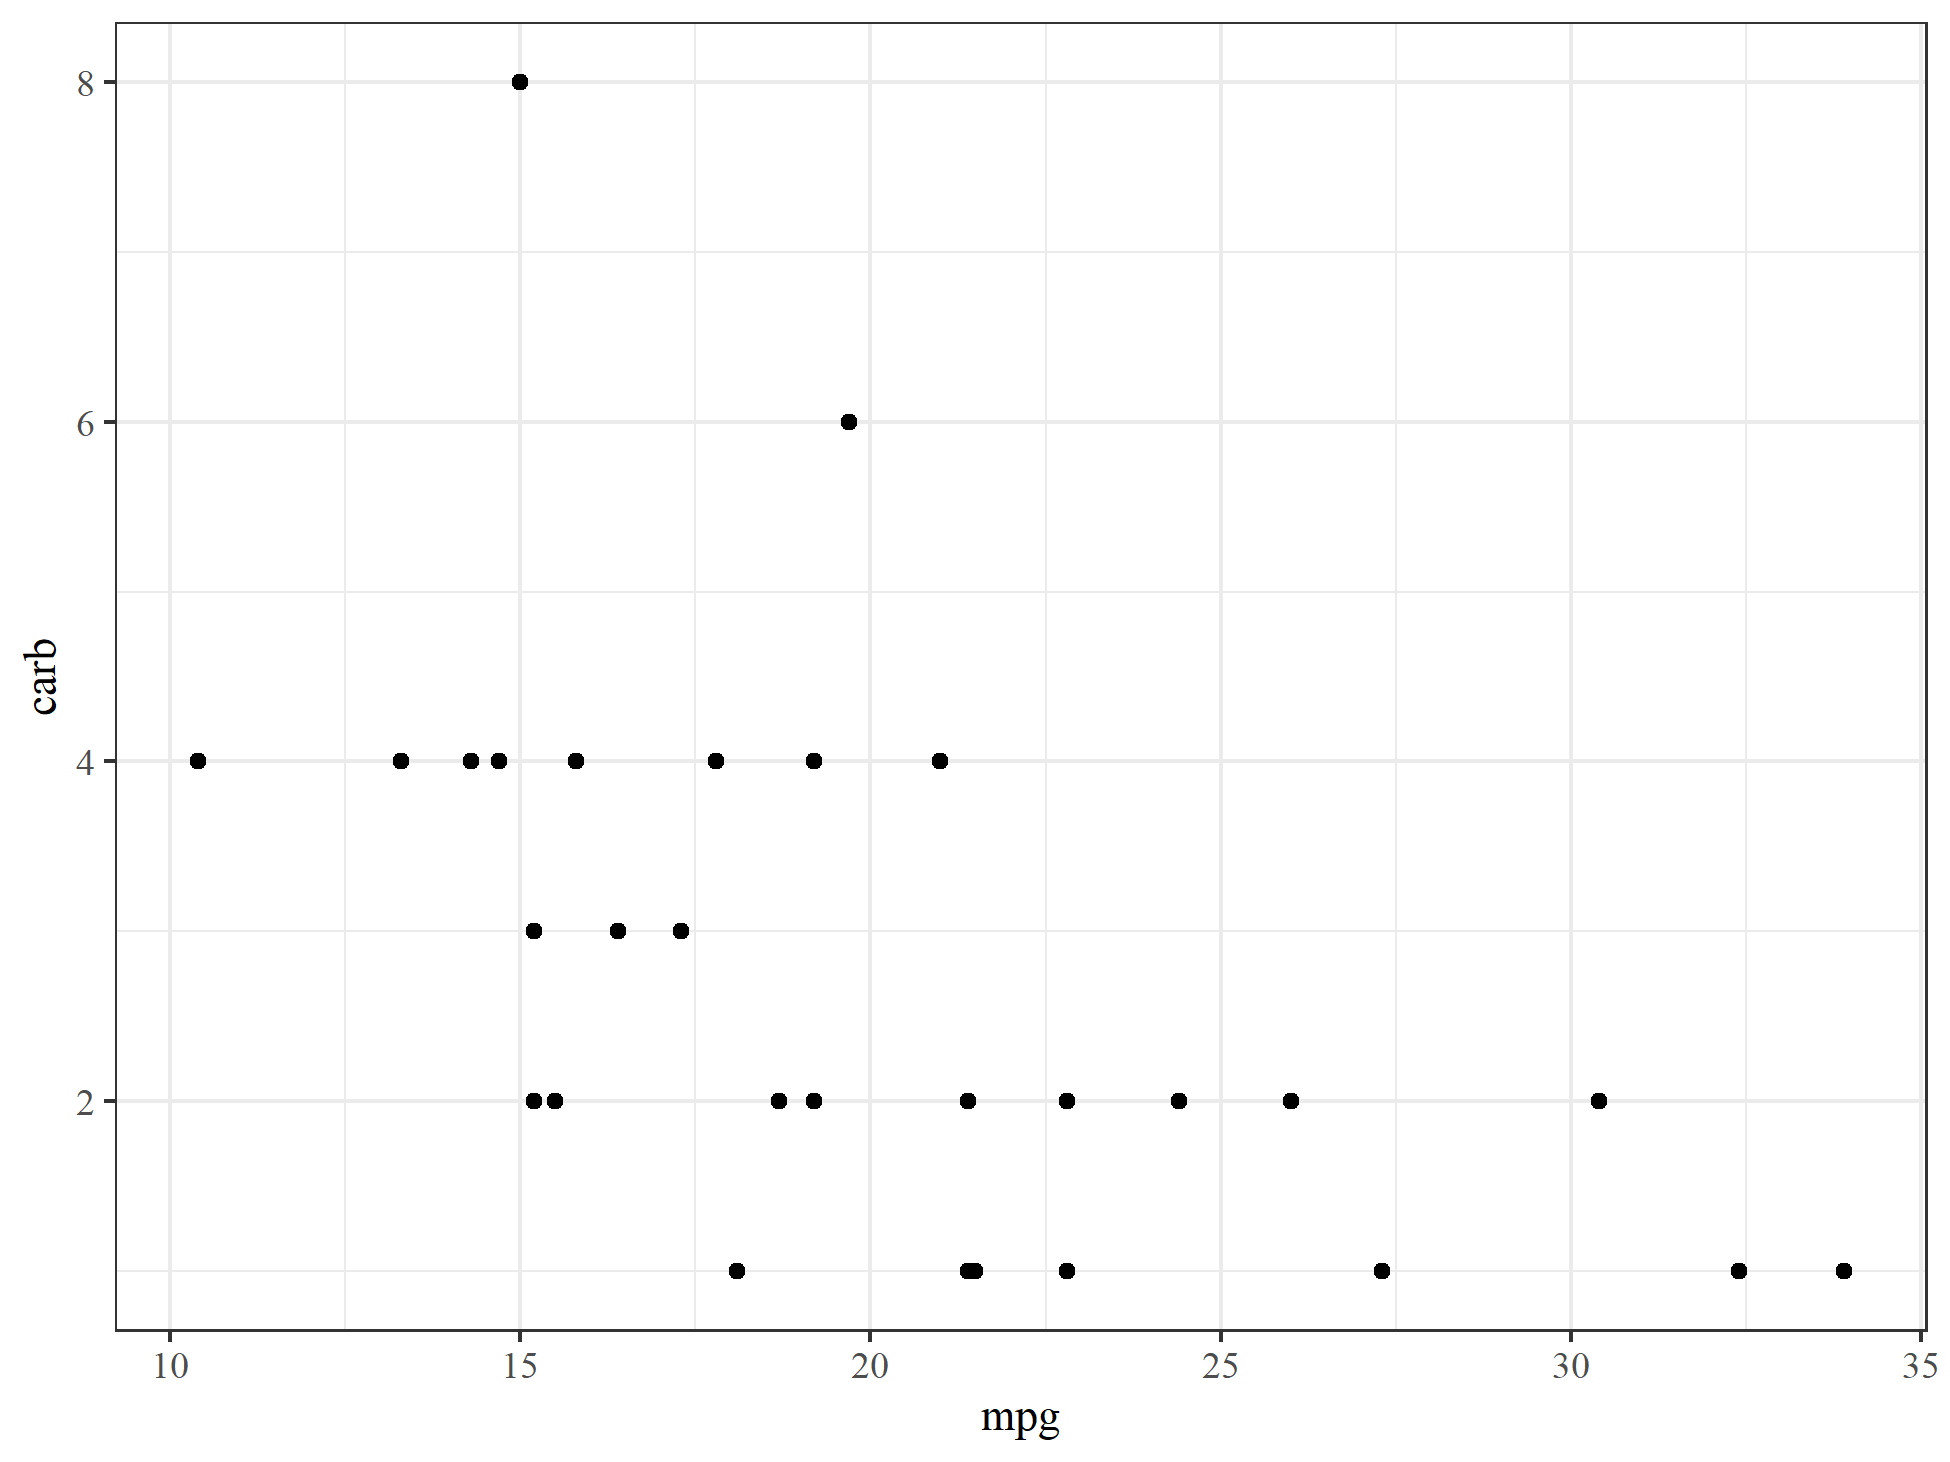
\includegraphics[width = \linewidth]{cookbook_files/figure-latex/carb-fig1-1}
\caption{Bal oldali ábra}
\label{fig:bar2_a6}
\end{figure}

\columnbreak

\begin{figure}[H]
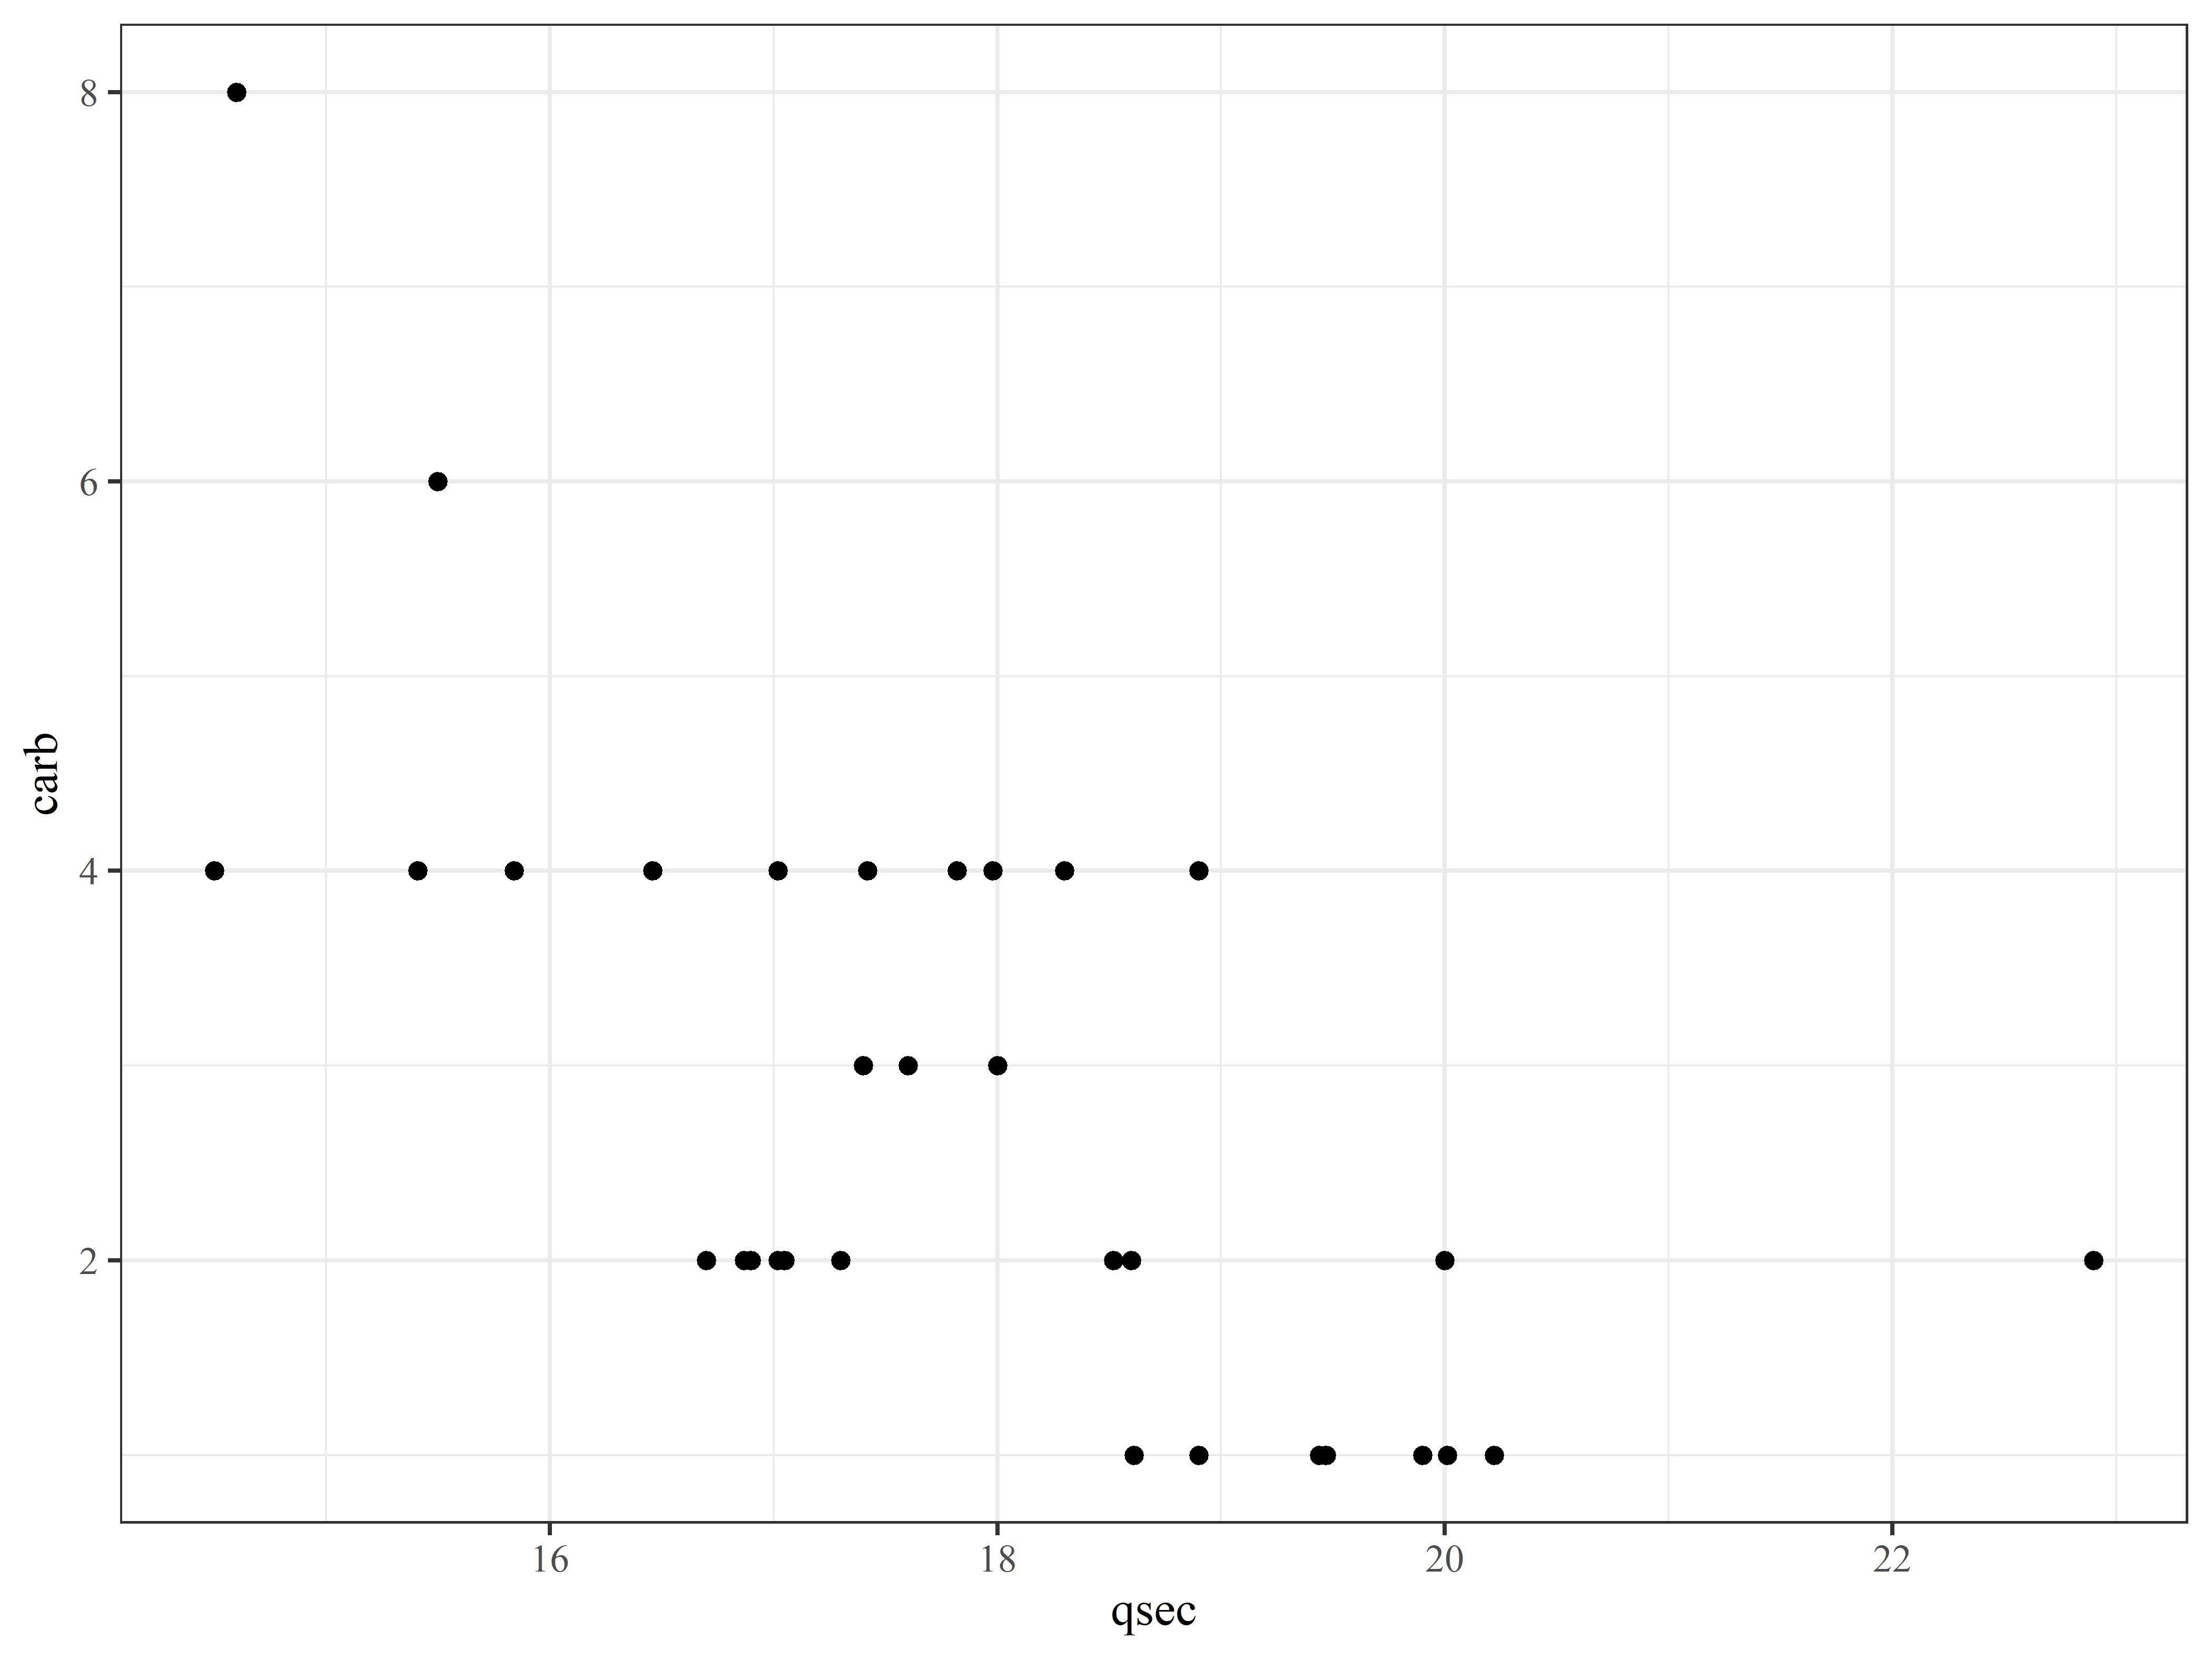
\includegraphics[width = \linewidth]{cookbook_files/figure-latex/carb-fig1-2}
\centering
\caption{Jobb oldali ábra}
\label{fig:bar2_b6}
\end{figure}
\end{multicols}
\end{figure}

És még hivatkozni is tudunk a(z) \ref{fig:param_plot16}. ábrára.

\begin{figure}[H]

{\centering 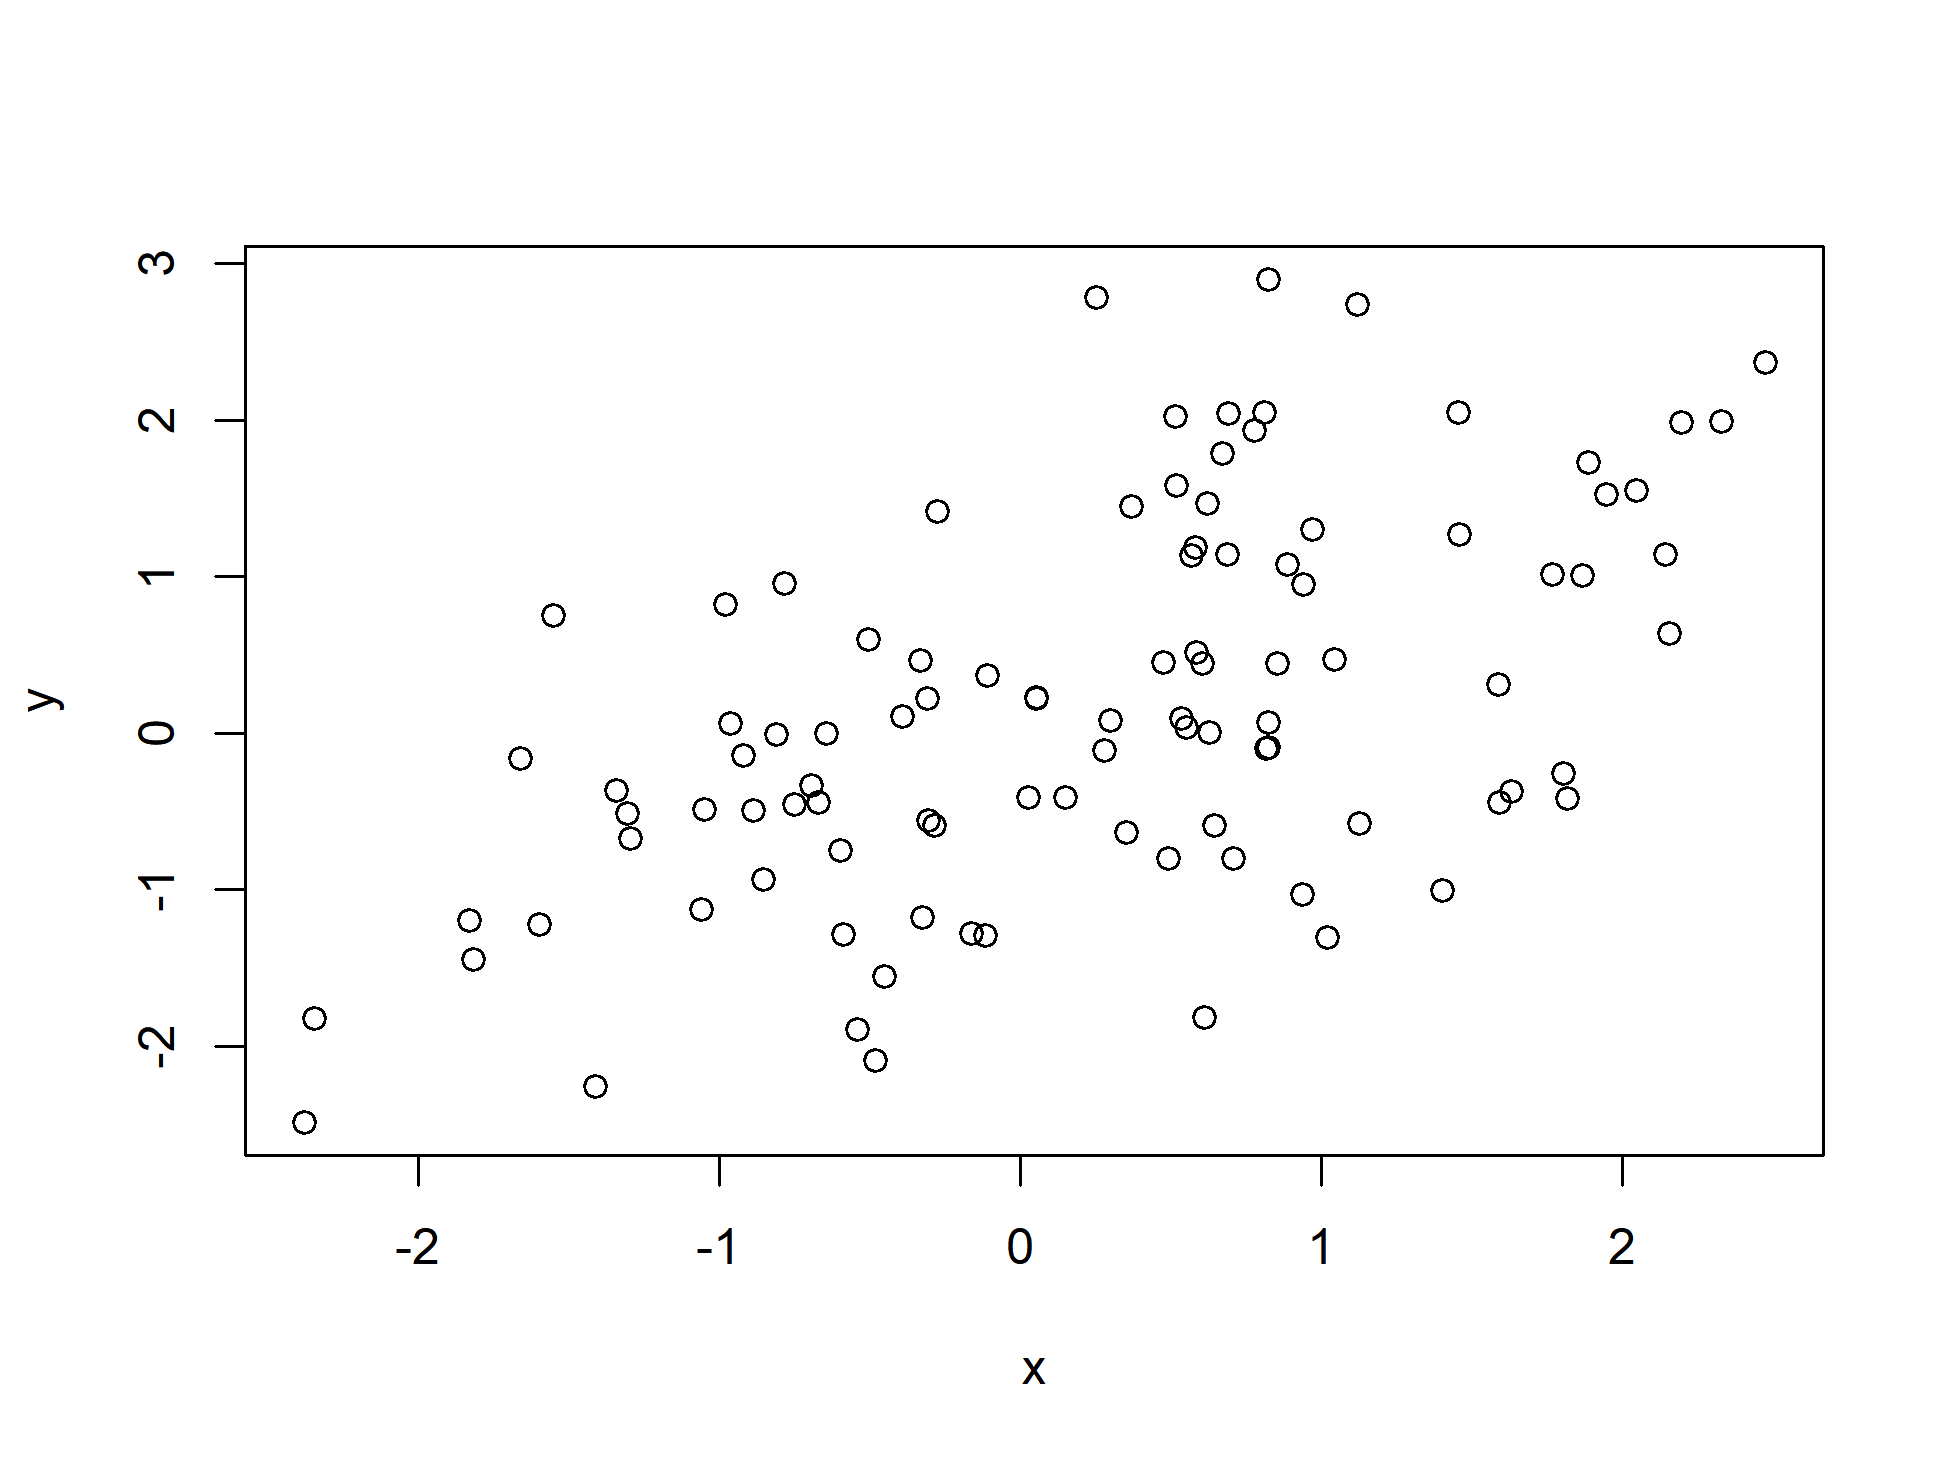
\includegraphics[width=0.9\linewidth]{cookbook_files/figure-latex/referenced_chunk-1} 

}

\caption{Executive graph for executive thoughts}\label{fig:referenced_chunk}
\end{figure}

\hypertarget{notes}{%
\section{Notes}\label{notes}}

The MD5 checksum of the database used:

\begin{verbatim}
## C:/OneDrive_DKM/-/Dinamikus Kiválóság Menedzsment - General/Stats_R/R/MartysCookbook/inst/extdata/Iris.xls 
##                                                                         "1ed4b9d5418675e017479de339aff352"
\end{verbatim}

Other information regarding the compilation of this document:

Analyses were conducted using the R Statistical language (version 4.3.0;
R Core Team, 2023) on Windows 10 x64 (build 19045), using the packages
lme4 (version 1.1.33; Bates D et al., 2015), Matrix (version 1.5.4.1;
Bates D et al., 2023), effects (version 4.2.2; Fox J, Weisberg S, 2019),
carData (version 3.0.5; Fox J et al., 2022), lubridate (version 1.9.2;
Grolemund G, Wickham H, 2011), DHARMa (version 0.4.6; Hartig F, 2022),
huxtable (version 5.5.2; Hugh-Jones D, 2022), labelled (version 2.11.0;
Larmarange J, 2023), emmeans (version 1.8.6; Lenth R, 2023), nlme
(version 3.1.162; Pinheiro J et al., 2023), gtsummary (version 1.7.1;
Sjoberg D et al., 2021), ggplot2 (version 3.4.2; Wickham H, 2016),
readxl (version 1.4.2; Wickham H, Bryan J, 2023), roxygen2 (version
7.2.3; Wickham H et al., 2022), dplyr (version 1.1.2; Wickham H et al.,
2023) and knitr (version 1.43; Xie Y, 2023).

\hypertarget{references}{%
\subsection{References}\label{references}}

\begin{itemize}
\tightlist
\item
  Bates D, Mächler M, Bolker B, Walker S (2015). ``Fitting Linear
  Mixed-Effects Models Using lme4.'' \emph{Journal of Statistical
  Software}, \emph{67}(1), 1-48. .
\item
  Bates D, Maechler M, Jagan M (2023). \emph{Matrix: Sparse and Dense
  Matrix Classes and Methods}. R package version 1.5-4.1,
  \url{https://CRAN.R-project.org/package=Matrix}.
\item
  Fox J, Weisberg S (2019). \emph{An R Companion to Applied Regression},
  3rd edition. Sage, Thousand Oaks CA.
  \url{https://socialsciences.mcmaster.ca/jfox/Books/Companion/index.html}.
\item
  Fox J, Weisberg S, Price B (2022). \emph{carData: Companion to Applied
  Regression Data Sets}. R package version 3.0-5,
  \url{https://CRAN.R-project.org/package=carData}.
\item
  Grolemund G, Wickham H (2011). ``Dates and Times Made Easy with
  lubridate.'' \emph{Journal of Statistical Software}, \emph{40}(3),
  1-25. \url{https://www.jstatsoft.org/v40/i03/}.
\item
  Hartig F (2022). \emph{DHARMa: Residual Diagnostics for Hierarchical
  (Multi-Level / Mixed) Regression Models}. R package version 0.4.6,
  \url{https://CRAN.R-project.org/package=DHARMa}.
\item
  Hugh-Jones D (2022). \emph{huxtable: Easily Create and Style Tables
  for LaTeX, HTML and Other Formats}. R package version 5.5.2,
  \url{https://CRAN.R-project.org/package=huxtable}.
\item
  Larmarange J (2023). \emph{labelled: Manipulating Labelled Data}. R
  package version 2.11.0,
  \url{https://CRAN.R-project.org/package=labelled}.
\item
  Lenth R (2023). \emph{emmeans: Estimated Marginal Means, aka
  Least-Squares Means}. R package version 1.8.6,
  \url{https://CRAN.R-project.org/package=emmeans}.
\item
  Pinheiro J, Bates D, R Core Team (2023). \emph{nlme: Linear and
  Nonlinear Mixed Effects Models}. R package version 3.1-162,
  \url{https://CRAN.R-project.org/package=nlme}.
\item
  R Core Team (2023). \emph{R: A Language and Environment for
  Statistical Computing}. R Foundation for Statistical Computing,
  Vienna, Austria. \url{https://www.R-project.org/}.
\item
  Sjoberg D, Whiting K, Curry M, Lavery J, Larmarange J (2021).
  ``Reproducible Summary Tables with the gtsummary Package.'' \emph{The
  R Journal}, \emph{13}, 570-580. ,
  \url{https://doi.org/10.32614/RJ-2021-053}.
\item
  Wickham H (2016). \emph{ggplot2: Elegant Graphics for Data Analysis}.
  Springer-Verlag New York. ISBN 978-3-319-24277-4,
  \url{https://ggplot2.tidyverse.org}.
\item
  Wickham H, Bryan J (2023). \emph{readxl: Read Excel Files}. R package
  version 1.4.2, \url{https://CRAN.R-project.org/package=readxl}.
\item
  Wickham H, Danenberg P, Csárdi G, Eugster M (2022). \emph{roxygen2:
  In-Line Documentation for R}. R package version 7.2.3,
  \url{https://CRAN.R-project.org/package=roxygen2}.
\item
  Wickham H, François R, Henry L, Müller K, Vaughan D (2023).
  \emph{dplyr: A Grammar of Data Manipulation}. R package version 1.1.2,
  \url{https://CRAN.R-project.org/package=dplyr}.
\item
  Xie Y (2023). \emph{knitr: A General-Purpose Package for Dynamic
  Report Generation in R}. R package version 1.43,
  \url{https://yihui.org/knitr/}.
\end{itemize}

This document was compiled at:

\begin{verbatim}
[1] "2023-06-09 13:55:45 CEST"
\end{verbatim}

\hypertarget{appendix}{%
\section{Appendix}\label{appendix}}

This is how put all your code into an appendix.

\begin{Shaded}
\begin{Highlighting}[]
\CommentTok{\# https://dotcms.com/docs/latest/markdown{-}syntax  }
\CommentTok{\# https://yihui.org/knitr/options/ }
\CommentTok{\# https://zbib.org/}
\CommentTok{\# https://www.r{-}bloggers.com/2019/09/first{-}world{-}problems{-}very{-}long{-}rmarkdown{-}documents/ }


\CommentTok{\# \# For citations insert this into the yaml header (without spaces)}
\CommentTok{\# \# And make a book.bib file to the location of the mother .rmd}
\CommentTok{\# bibliography: book.bib}
\CommentTok{\# biblio{-}style: apalike}
\CommentTok{\# link{-}citations: yes}

\FunctionTok{source}\NormalTok{(here}\SpecialCharTok{::}\FunctionTok{here}\NormalTok{(}\StringTok{"inst"}\NormalTok{,}\StringTok{"functions"}\NormalTok{,}\StringTok{"load\_stuff.r"}\NormalTok{))}

\NormalTok{knitr}\SpecialCharTok{::}\NormalTok{opts\_chunk}\SpecialCharTok{$}\FunctionTok{set}\NormalTok{(}
    \AttributeTok{echo =} \ConstantTok{FALSE}\NormalTok{,                           }\CommentTok{\# Ne mutassa a kódokat}
    \AttributeTok{cached =} \ConstantTok{FALSE}\NormalTok{,                 }\DocumentationTok{\#\#\#!!!  \# Ne cache{-}eljen}
    \AttributeTok{warning =} \ConstantTok{FALSE}\NormalTok{,                        }\CommentTok{\# Ne írja ki a warningokat}
    \AttributeTok{message =} \ConstantTok{FALSE}\NormalTok{, }
    \AttributeTok{fig.align =} \StringTok{\textquotesingle{}center\textquotesingle{}}\NormalTok{,                   }\CommentTok{\# Ábra középre rendezése}
    \AttributeTok{out.width =} \StringTok{\textquotesingle{}90\%\textquotesingle{}}\NormalTok{,                      }\CommentTok{\# Ábra szélessége, alter.: \#fig.fullwidth = TRUE,}
    \AttributeTok{fig.asp =}\NormalTok{ .}\DecValTok{75}\NormalTok{,                          }\CommentTok{\# Ábra Hossz/szélesség}
    \AttributeTok{tidy.opts =} \FunctionTok{list}\NormalTok{(}\AttributeTok{width.cutoff =} \DecValTok{60}\NormalTok{),    }\CommentTok{\# legyenek 60 karakter szélességűre tördelve}
    \AttributeTok{tidy =} \StringTok{"styler"}\NormalTok{,                        }\CommentTok{\# legyenek clean codingra megformázva}
    \AttributeTok{dev =} \StringTok{\textquotesingle{}png\textquotesingle{}}\NormalTok{,}\CommentTok{\#\textquotesingle{}tiff\textquotesingle{},                            \# PNG legyen az alapértelmezett képformátum}
    \AttributeTok{compression =} \StringTok{\textquotesingle{}lzw\textquotesingle{}}\NormalTok{,}
    \AttributeTok{dpi =} \DecValTok{300}\NormalTok{,                              }\CommentTok{\# a PNG képek elég jó minőségűek legyenek}
    \AttributeTok{fig.pos =} \StringTok{\textquotesingle{}H\textquotesingle{}}                           \CommentTok{\# nem próbálja az ábrákat az oldal tetejére tenni}
\NormalTok{  )}


\NormalTok{graphics\_path }\OtherTok{\textless{}{-}} \StringTok{"../inst/figure/"}            \CommentTok{\# a máshonnan származó ábrák elérési útja}
\NormalTok{graphics\_output\_path }\OtherTok{\textless{}{-}} \StringTok{"cookbook\_files/figure{-}latex/"} \CommentTok{\# az itt generált ábrák elérési útja}

\FunctionTok{options}\NormalTok{(}\AttributeTok{scipen =} \DecValTok{1}\NormalTok{) }\CommentTok{\# Require 5 instead of 4 for scientific notation (eg. for p{-}values)}
\FunctionTok{options}\NormalTok{(}\AttributeTok{digits =} \DecValTok{3}\NormalTok{) }\CommentTok{\# default no. of digits (!) }
\FunctionTok{options}\NormalTok{(}\AttributeTok{encoding =} \StringTok{"UTF{-}8"}\NormalTok{) }

\FunctionTok{plot}\NormalTok{(x,y)}

\FunctionTok{save.image}\NormalTok{( }\AttributeTok{file =}\NormalTok{ here}\SpecialCharTok{::}\FunctionTok{here}\NormalTok{(}\StringTok{"inst"}\NormalTok{,}\StringTok{"states"}\NormalTok{, }\StringTok{"before\_chap1.Rdata"}\NormalTok{))}

\NormalTok{valtozok }\OtherTok{\textless{}{-}} \FunctionTok{c}\NormalTok{(}\StringTok{"cyl"}\NormalTok{, }\StringTok{"gear"}\NormalTok{, }\StringTok{"carb"}\NormalTok{)}
\NormalTok{out }\OtherTok{\textless{}{-}} \ConstantTok{NULL}

\ControlFlowTok{for}\NormalTok{ (i }\ControlFlowTok{in} \DecValTok{1}\SpecialCharTok{:}\FunctionTok{length}\NormalTok{(valtozok)) \{}
\NormalTok{  out }\OtherTok{\textless{}{-}} \FunctionTok{c}\NormalTok{(out, }\FunctionTok{paste0}\NormalTok{(}\StringTok{"}\SpecialCharTok{\textbackslash{}n}\StringTok{\#\#\# "}\NormalTok{, valtozok[i], }\StringTok{"}\SpecialCharTok{\textbackslash{}n}\StringTok{"}\NormalTok{)) }\CommentTok{\# Defining "title"}
\NormalTok{  params }\OtherTok{\textless{}{-}} \FunctionTok{list}\NormalTok{(}\AttributeTok{x              =}\NormalTok{ valtozok[i],}
                 \AttributeTok{top\_level      =} \DecValTok{4}\NormalTok{,}
                 \AttributeTok{figname\_prefix =}\NormalTok{ valtozok[i])}
\NormalTok{  out }\OtherTok{\textless{}{-}} \FunctionTok{c}\NormalTok{(out,}
\NormalTok{           knitr}\SpecialCharTok{::}\FunctionTok{knit\_child}\NormalTok{(here}\SpecialCharTok{::}\FunctionTok{here}\NormalTok{(}\StringTok{"inst"}\NormalTok{,}\StringTok{\textquotesingle{}cyclic\_chap2.Rmd\textquotesingle{}}\NormalTok{),}
                             \AttributeTok{quiet =}\NormalTok{ T))}
\NormalTok{\}}
\NormalTok{out }\OtherTok{\textless{}{-}} \FunctionTok{paste}\NormalTok{(out, }\AttributeTok{collapse =} \StringTok{"}\SpecialCharTok{\textbackslash{}n}\StringTok{"}\NormalTok{)}

\FunctionTok{set.seed}\NormalTok{(}\DecValTok{12345}\NormalTok{)}

\NormalTok{x }\OtherTok{\textless{}{-}} \FunctionTok{rnorm}\NormalTok{(}\DecValTok{100}\NormalTok{)}
\NormalTok{y }\OtherTok{\textless{}{-}} \FloatTok{0.5} \SpecialCharTok{*}\NormalTok{ x }\SpecialCharTok{+} \FunctionTok{rnorm}\NormalTok{(}\DecValTok{100}\NormalTok{)}

\FunctionTok{plot}\NormalTok{(x,y, }\AttributeTok{main =} \StringTok{"Important plot to reference before its compiled"}\NormalTok{)}

\NormalTok{tools}\SpecialCharTok{::}\FunctionTok{md5sum}\NormalTok{(here}\SpecialCharTok{::}\FunctionTok{here}\NormalTok{(}\StringTok{"inst"}\NormalTok{,}\StringTok{"extdata"}\NormalTok{,}\StringTok{"Iris.xls"}\NormalTok{))}
\NormalTok{knitr}\SpecialCharTok{::}\NormalTok{opts\_chunk}\SpecialCharTok{$}\FunctionTok{set}\NormalTok{(}\AttributeTok{comment =} \ConstantTok{NA}\NormalTok{)}
\FunctionTok{sessionInfo}\NormalTok{() }\SpecialCharTok{\%\textgreater{}\%}\NormalTok{ report}\SpecialCharTok{::}\FunctionTok{report}\NormalTok{() }\SpecialCharTok{\%\textgreater{}\%} \FunctionTok{cat}\NormalTok{()}

\FunctionTok{Sys.time}\NormalTok{()}
\FunctionTok{save.image}\NormalTok{(}\AttributeTok{file =}\NormalTok{ here}\SpecialCharTok{::}\FunctionTok{here}\NormalTok{(}\StringTok{"inst"}\NormalTok{,}\StringTok{"states"}\NormalTok{,}\StringTok{"cookbook\_out.Rdata"}\NormalTok{))}



\FunctionTok{source}\NormalTok{(here}\SpecialCharTok{::}\FunctionTok{here}\NormalTok{(}\StringTok{"inst"}\NormalTok{,}\StringTok{"functions"}\NormalTok{,}\StringTok{"load\_stuff.r"}\NormalTok{))}
\FunctionTok{load}\NormalTok{( }\AttributeTok{file =}\NormalTok{ here}\SpecialCharTok{::}\FunctionTok{here}\NormalTok{(}\StringTok{"inst"}\NormalTok{,}\StringTok{"states"}\NormalTok{, }\StringTok{"before\_chap1.Rdata"}\NormalTok{))}

\NormalTok{graphics\_output\_path }\OtherTok{\textless{}{-}} \StringTok{"cookbook\_files/figure{-}latex/"} \CommentTok{\# az itt generált ábrák elérési útja}

\CommentTok{\# This is an example of factor releveling snatched from}
\CommentTok{\# https://www.tutorialspoint.com/r/r\_factors.htm}

\NormalTok{data\_f }\OtherTok{\textless{}{-}} \FunctionTok{c}\NormalTok{(}\StringTok{"East"}\NormalTok{,}\StringTok{"West"}\NormalTok{,}\StringTok{"East"}\NormalTok{,}\StringTok{"North"}\NormalTok{,}\StringTok{"North"}\NormalTok{,}\StringTok{"East"}\NormalTok{,}\StringTok{"West"}\NormalTok{,}
   \StringTok{"West"}\NormalTok{,}\StringTok{"West"}\NormalTok{,}\StringTok{"East"}\NormalTok{,}\StringTok{"North"}\NormalTok{)}
\CommentTok{\# Create the factors}
\NormalTok{factor\_data }\OtherTok{\textless{}{-}} \FunctionTok{factor}\NormalTok{(data\_f)}
\FunctionTok{print}\NormalTok{(factor\_data)}

\CommentTok{\# Apply the factor function with required order of the level.}
\NormalTok{new\_order\_data }\OtherTok{\textless{}{-}} \FunctionTok{factor}\NormalTok{(factor\_data,}\AttributeTok{levels =} \FunctionTok{c}\NormalTok{(}\StringTok{"East"}\NormalTok{,}\StringTok{"West"}\NormalTok{,}\StringTok{"North"}\NormalTok{))}
\FunctionTok{print}\NormalTok{(new\_order\_data)}



\CommentTok{\# First subplot}
\NormalTok{fig\_1a }\OtherTok{\textless{}{-}} 
\NormalTok{data }\SpecialCharTok{\%\textgreater{}\%}
  \FunctionTok{ggplot}\NormalTok{( }\FunctionTok{aes}\NormalTok{( }\AttributeTok{x =}\NormalTok{ species\_no,}
               \AttributeTok{y =}\NormalTok{ petal\_width)) }\SpecialCharTok{+}
  \CommentTok{\# Theme}
\NormalTok{  theme\_default\_ggplot }\SpecialCharTok{+}
  \CommentTok{\# Layers}
  \FunctionTok{geom\_point}\NormalTok{() }\SpecialCharTok{+}
  \CommentTok{\# axis wrangling}
  \FunctionTok{scale\_y\_continuous}\NormalTok{( }
    \CommentTok{\# setting up a custom log transform ( the pre{-}defined results in error somehow...)}
    \AttributeTok{trans =}\NormalTok{ scales}\SpecialCharTok{::}\FunctionTok{trans\_new}\NormalTok{(}\StringTok{"expmar"}\NormalTok{, exp,}
            \ControlFlowTok{function}\NormalTok{(x)\{}
                \CommentTok{\#print(paste("isq",x))  \#debug statement}
\NormalTok{                x }\OtherTok{\textless{}{-}}\FunctionTok{ifelse}\NormalTok{(x}\SpecialCharTok{\textless{}}\DecValTok{0}\NormalTok{, }\DecValTok{0}\NormalTok{, x)}
                \FunctionTok{log}\NormalTok{(x)}
\NormalTok{              \})}
\NormalTok{  ) }\SpecialCharTok{+}
  \CommentTok{\# description(s)}
  \FunctionTok{labs}\NormalTok{( }\AttributeTok{x =} \StringTok{"Species on this axis wahaha"}\NormalTok{,}
        \AttributeTok{y =} \StringTok{"log transformed variable"}\NormalTok{)}


\CommentTok{\# Second subplot}
\NormalTok{fig\_1b }\OtherTok{\textless{}{-}} 
\NormalTok{data }\SpecialCharTok{\%\textgreater{}\%}
  \FunctionTok{ggplot}\NormalTok{( }\FunctionTok{aes}\NormalTok{( }\AttributeTok{x =}\NormalTok{ species\_no,}
               \AttributeTok{y =}\NormalTok{ petal\_width)) }\SpecialCharTok{+}
  \CommentTok{\# Theme}
\NormalTok{  theme\_default\_ggplot }\SpecialCharTok{+}
  \FunctionTok{theme}\NormalTok{( }\AttributeTok{legend.position=}\StringTok{"bottom"}\NormalTok{) }\SpecialCharTok{+} \CommentTok{\# custom legend position if needed}
  \CommentTok{\# Layers}
  \FunctionTok{geom\_point}\NormalTok{() }\SpecialCharTok{+}
  \CommentTok{\# axis wrangling}
  \FunctionTok{scale\_y\_continuous}\NormalTok{( }
    \AttributeTok{limits =} \FunctionTok{c}\NormalTok{( }\DecValTok{0}\NormalTok{,}\FloatTok{3.3}\NormalTok{),}
    \AttributeTok{breaks =} \FunctionTok{c}\NormalTok{( }\DecValTok{0}\NormalTok{, .}\DecValTok{6}\NormalTok{, }\DecValTok{1}\NormalTok{, }\FloatTok{1.8}\NormalTok{, }\FloatTok{2.6}\NormalTok{)}
\NormalTok{  ) }\SpecialCharTok{+}
  \CommentTok{\# description(s)}
  \FunctionTok{labs}\NormalTok{( }\AttributeTok{x =} \StringTok{"Species on the other copy of the axis wahaha"}\NormalTok{,}
        \AttributeTok{y =} \StringTok{"variable on original scale"}\NormalTok{)}

\CommentTok{\# Demonstrating arranging plots}
\NormalTok{fig\_1comp }\OtherTok{\textless{}{-}} 
\NormalTok{  ggpubr}\SpecialCharTok{::}\FunctionTok{ggarrange}\NormalTok{(fig\_1a, fig\_1b, }
          \CommentTok{\#labels = c("", ""), \# if you\textquotesingle{}d like to omit the labels}
          \AttributeTok{labels =} \StringTok{"AUTO"}\NormalTok{,}
          \AttributeTok{ncol =} \DecValTok{2}\NormalTok{, }\AttributeTok{nrow =} \DecValTok{1}\NormalTok{)}

\CommentTok{\# calling the plot}
\NormalTok{(fig\_1comp)}


\NormalTok{data\_local }\OtherTok{\textless{}{-}} \FunctionTok{data.frame}\NormalTok{( }\AttributeTok{x =} \FunctionTok{rnorm}\NormalTok{(}\DecValTok{100}\NormalTok{)) }\SpecialCharTok{\%\textgreater{}\%}
                \FunctionTok{mutate}\NormalTok{(}\AttributeTok{y =}\NormalTok{ x }\SpecialCharTok{*} \FloatTok{0.5} \SpecialCharTok{+} \FunctionTok{rnorm}\NormalTok{(}\DecValTok{100}\NormalTok{))}

\NormalTok{data\_local }\SpecialCharTok{\%\textgreater{}\%}
  \FunctionTok{ggplot}\NormalTok{( }\FunctionTok{aes}\NormalTok{(}\AttributeTok{x=}\NormalTok{x,}\AttributeTok{y=}\NormalTok{y)) }\SpecialCharTok{+}
\NormalTok{    theme\_default\_ggplot }\SpecialCharTok{+}
    \FunctionTok{geom\_point}\NormalTok{()}

\FunctionTok{hist}\NormalTok{(data\_local}\SpecialCharTok{$}\NormalTok{x)}



\FunctionTok{tbl\_summary}\NormalTok{( data, }\AttributeTok{by =}\NormalTok{ species\_char) }\SpecialCharTok{\%\textgreater{}\%} 
  \FunctionTok{martys\_table\_style}\NormalTok{(}\AttributeTok{caption. =} 
                       \StringTok{"Plot without much thought or meaning"}\NormalTok{) }\SpecialCharTok{\%\textgreater{}\%} 
  \CommentTok{\# You can \textquotesingle{}overwrite\textquotesingle{} setting which don\textquotesingle{}t conflict your defaults}
  \FunctionTok{set\_font\_size}\NormalTok{(}\DecValTok{7}\NormalTok{) }\SpecialCharTok{\%\textgreater{}\%}
  \DocumentationTok{\#\#\#\#\#\# row\_spec(0, bold = T, font\_size = 7)\# \%\textgreater{}\% \# Dis crashes the whole thing}
   \FunctionTok{set\_width}\NormalTok{(.}\DecValTok{4}\NormalTok{)}


\FunctionTok{head}\NormalTok{(mtcars) }\SpecialCharTok{\%\textgreater{}\%}
  \FunctionTok{martys\_table\_style}\NormalTok{(}\AttributeTok{caption. =} \StringTok{"Dis be the second table"}\NormalTok{)}



\CommentTok{\# Calling the plot}
\NormalTok{plot. }\OtherTok{\textless{}{-}} 
\NormalTok{  data }\SpecialCharTok{\%\textgreater{}\%}
    \FunctionTok{ggplot}\NormalTok{( }\FunctionTok{aes}\NormalTok{(}\AttributeTok{x =}\NormalTok{ species\_char, }\AttributeTok{y =}\NormalTok{ sepal\_width, }
                \AttributeTok{color =}\NormalTok{ species\_char, }\AttributeTok{fill =}\NormalTok{ species\_char)) }\SpecialCharTok{+} 
\NormalTok{    theme\_default\_ggplot }\SpecialCharTok{+}
    \CommentTok{\# half smoothed density}
\NormalTok{    ggdist}\SpecialCharTok{::}\FunctionTok{stat\_halfeye}\NormalTok{(}
      \DocumentationTok{\#\# bandwidth}
      \AttributeTok{adjust =} \FloatTok{0.6}\NormalTok{,}
      \AttributeTok{justification =} \SpecialCharTok{{-}}\NormalTok{.}\DecValTok{2}\NormalTok{,}
      \AttributeTok{.width =} \DecValTok{0}\NormalTok{,}
      \AttributeTok{width =}\NormalTok{ .}\DecValTok{25}
\NormalTok{    ) }\SpecialCharTok{+} 
    \CommentTok{\# Boxplot}
    \FunctionTok{geom\_boxplot}\NormalTok{( }\AttributeTok{width =}\NormalTok{ .}\DecValTok{08}\NormalTok{,}
                  \CommentTok{\# remove outliers from boxplot}
                  \AttributeTok{outlier.color =} \ConstantTok{NA}\NormalTok{,}
                  \AttributeTok{alpha =}\NormalTok{ .}\DecValTok{5}\NormalTok{) }\SpecialCharTok{+}
    \CommentTok{\# Dotplot}
\NormalTok{    ggdist}\SpecialCharTok{::}\FunctionTok{stat\_dots}\NormalTok{(}
      \AttributeTok{side =} \StringTok{"left"}\NormalTok{, }
      \AttributeTok{dotsize =}\NormalTok{ .}\DecValTok{1}\NormalTok{, }
      \AttributeTok{justification =} \FloatTok{1.12}\NormalTok{, }
      \AttributeTok{binwidth =}\NormalTok{ .}\DecValTok{125}
\NormalTok{    ) }\SpecialCharTok{+}
    \FunctionTok{labs}\NormalTok{( }
      \CommentTok{\# coord\_flip doesn\textquotesingle{}t affect this ;)}
      \AttributeTok{x =} \StringTok{"Species"}\NormalTok{,}
      \AttributeTok{y =} \StringTok{"Width of sepals (mm)"}\NormalTok{,}
      \CommentTok{\# Including latex, see https://cran.r{-}project.org/web/packages/latex2exp/vignettes/using{-}latex2exp.html}
      \AttributeTok{caption =}\NormalTok{ latex2exp}\SpecialCharTok{::}\FunctionTok{TeX}\NormalTok{(r}\StringTok{"($   }\SpecialCharTok{\textbackslash{}a}\StringTok{lpha\^{}\{5{-}i\_j\}\textbackslash{} is\textbackslash{} a\textbackslash{} nifty\textbackslash{} string   $)"}\NormalTok{),}
      \AttributeTok{title =} \StringTok{"Its not better to set titles in ggplot2..."}
\NormalTok{      ) }\SpecialCharTok{+}
    \FunctionTok{scale\_y\_continuous}\NormalTok{( }
      \AttributeTok{breaks =} \FunctionTok{c}\NormalTok{(}\DecValTok{0}\NormalTok{,}\DecValTok{1}\NormalTok{,}\DecValTok{2}\NormalTok{,}\DecValTok{3}\NormalTok{,}\DecValTok{4}\NormalTok{,}\DecValTok{5}\NormalTok{), }
      \AttributeTok{limits =} \FunctionTok{c}\NormalTok{(}\DecValTok{0}\NormalTok{,}\DecValTok{5}\NormalTok{)) }\SpecialCharTok{+}
    \FunctionTok{coord\_flip}\NormalTok{()}


\NormalTok{(plot.)}


\FunctionTok{library}\NormalTok{(lme4)}

\NormalTok{mod }\OtherTok{\textless{}{-}} \FunctionTok{lmer}\NormalTok{(}
\NormalTok{  petal\_width }\SpecialCharTok{\textasciitilde{}}
\NormalTok{    petal\_length }\SpecialCharTok{+}
\NormalTok{    sepal\_width }\SpecialCharTok{+}
\NormalTok{    (}\DecValTok{1} \SpecialCharTok{|}\NormalTok{ mock\_ID),}
\NormalTok{  data}
\NormalTok{)}


\CommentTok{\#Output is in html...}
\NormalTok{sjPlot}\SpecialCharTok{::}\FunctionTok{tab\_model}\NormalTok{(mod,}
    \CommentTok{\# transform = "exp", \# makes stuff multiplicative}
    \AttributeTok{digits.re =} \DecValTok{3}\NormalTok{,}
    \AttributeTok{show.reflvl =} \ConstantTok{TRUE}\NormalTok{,}
    \AttributeTok{pred.labels =} \FunctionTok{list}\NormalTok{(}
      \StringTok{\textasciigrave{}}\AttributeTok{(Intercept)}\StringTok{\textasciigrave{}} \OtherTok{=} \StringTok{"Interceeeeept"}\NormalTok{,}
      \AttributeTok{petal\_length  =} \StringTok{"Length of petal"}\NormalTok{,}
      \AttributeTok{sepal\_width   =} \StringTok{"Width of sepal"}
\NormalTok{    ),}
    \AttributeTok{dv.labels =} \StringTok{"Width of petal (mm)"}\NormalTok{,}
    \AttributeTok{df.method =} \StringTok{"kr"}\NormalTok{, }\CommentTok{\# makes it somewhat more conservative I guess}
    \AttributeTok{title =} \StringTok{"Specification of an lmer model"}
\NormalTok{    , }\AttributeTok{show.p =} \ConstantTok{FALSE} \CommentTok{\# if you\textquotesingle{}re also skeptical of p{-}values}
\NormalTok{    , }\AttributeTok{bootstrap =} \ConstantTok{TRUE}
\NormalTok{    , }\AttributeTok{iterations =} \DecValTok{100} \CommentTok{\# actually works for lmer(!)}
\NormalTok{    , }\AttributeTok{file =}\NormalTok{ here}\SpecialCharTok{::}\FunctionTok{here}\NormalTok{(}\StringTok{"inst"}\NormalTok{,}\StringTok{"stuff"}\NormalTok{,}\StringTok{"temp.html"}\NormalTok{) }\CommentTok{\# have to export temporarily}
\NormalTok{  )}


  \CommentTok{\# The "webshot2" stuff needs to be done \textquotesingle{}invisibly\textquotesingle{} or else it }
  \CommentTok{\# spawns a copy of the previous image  }
\FunctionTok{invisible}\NormalTok{(\{}
  \CommentTok{\#taking a \textquotesingle{}snapshot\textquotesingle{} of the html and converting it to .png}
\NormalTok{  webshot2}\SpecialCharTok{::}\FunctionTok{webshot}\NormalTok{(}\AttributeTok{url=}\NormalTok{here}\SpecialCharTok{::}\FunctionTok{here}\NormalTok{(}\StringTok{"inst"}\NormalTok{,}\StringTok{"stuff"}\NormalTok{,}\StringTok{"temp.html"}\NormalTok{), }
                    \AttributeTok{cliprect =} \FunctionTok{c}\NormalTok{(}\DecValTok{0}\NormalTok{,}\DecValTok{0}\NormalTok{,}\DecValTok{400}\NormalTok{,}\DecValTok{400}\NormalTok{),}
                    \AttributeTok{file =}\NormalTok{ here}\SpecialCharTok{::}\FunctionTok{here}\NormalTok{(}\StringTok{"inst"}\NormalTok{,}\StringTok{"figure"}\NormalTok{,}\StringTok{"webshot.png"}\NormalTok{))}
\NormalTok{\})}



\CommentTok{\# How to predict an lmer model\textquotesingle{}s main effects based on bootstrap}
\CommentTok{\# slow as it gets if you like it pretty, introducing cache}

\NormalTok{CRANK }\OtherTok{\textless{}{-}} \DecValTok{30}

\NormalTok{pred }\OtherTok{\textless{}{-}} \FunctionTok{expand.grid}\NormalTok{(}
  \AttributeTok{petal\_length =} \FunctionTok{seq}\NormalTok{(}\DecValTok{1}\NormalTok{, }\DecValTok{5}\NormalTok{, }\AttributeTok{length.out =} \DecValTok{10}\NormalTok{),}
  \AttributeTok{sepal\_width  =} \FunctionTok{seq}\NormalTok{(}\DecValTok{1}\NormalTok{, }\DecValTok{5}\NormalTok{, }\AttributeTok{length.out =} \DecValTok{3}\NormalTok{)}
\NormalTok{)}

\NormalTok{pred\_out }\OtherTok{\textless{}{-}}\NormalTok{ ciTools}\SpecialCharTok{::}\FunctionTok{add\_ci}\NormalTok{(pred, mod,}
  \AttributeTok{includeRanef =} \ConstantTok{FALSE}\NormalTok{, }\AttributeTok{type =} \StringTok{"boot"}\NormalTok{,}
  \AttributeTok{nSims =}\NormalTok{ CRANK }\CommentTok{\# crank up in production}
\NormalTok{)}

\CommentTok{\# fig.show=\textquotesingle{}hide\textquotesingle{}}

\NormalTok{plot\_lmeoutpred }\OtherTok{\textless{}{-}} 
\NormalTok{  pred\_out }\SpecialCharTok{\%\textgreater{}\%}
    \FunctionTok{mutate}\NormalTok{( }
      \CommentTok{\# Recoding into factor the facetting value, labels will be based on the labels...}
      \AttributeTok{sepal\_width2 =} \FunctionTok{factor}\NormalTok{( sepal\_width, }\AttributeTok{labels =} \FunctionTok{c}\NormalTok{(}\StringTok{"Very small"}\NormalTok{, }
                                                     \StringTok{"Medium"}\NormalTok{, }
                                                     \StringTok{"Really large"}\NormalTok{))) }\SpecialCharTok{\%\textgreater{}\%}
    \FunctionTok{ggplot}\NormalTok{( }\FunctionTok{aes}\NormalTok{(}\AttributeTok{x =}\NormalTok{ petal\_length, }\AttributeTok{y =}\NormalTok{ pred, }
                \AttributeTok{group =}\NormalTok{ sepal\_width2, }\AttributeTok{color =}\NormalTok{ sepal\_width2}
\NormalTok{                , }\AttributeTok{fill =}\NormalTok{ sepal\_width)) }\SpecialCharTok{+}
\NormalTok{    theme\_default\_ggplot }\SpecialCharTok{+}
    \FunctionTok{geom\_line}\NormalTok{() }\SpecialCharTok{+}
    \FunctionTok{geom\_ribbon}\NormalTok{(}\AttributeTok{mapping =} \FunctionTok{aes}\NormalTok{( }\AttributeTok{ymin =}\NormalTok{ LCB0}\FloatTok{.025}\NormalTok{, }
                               \AttributeTok{ymax =}\NormalTok{ UCB0}\FloatTok{.975}\NormalTok{), }
                \AttributeTok{alpha =}\NormalTok{ .}\DecValTok{25}\NormalTok{, }
                \AttributeTok{colour =} \ConstantTok{NA}\NormalTok{) }\SpecialCharTok{+}
    \FunctionTok{facet\_grid}\NormalTok{( }\AttributeTok{facets =} \FunctionTok{c}\NormalTok{(}\StringTok{"sepal\_width2"}\NormalTok{), }\AttributeTok{labeller =}\NormalTok{ label\_value) }\SpecialCharTok{+}
    \FunctionTok{labs}\NormalTok{( }\AttributeTok{x =} \StringTok{"Length of Petal"}\NormalTok{,}
          \AttributeTok{y =} \StringTok{"Predicted sepal\_width)"}\NormalTok{,}
          \AttributeTok{caption =} \StringTok{"Confidence bands are conditional on the random effects(?)"}\NormalTok{)}

\NormalTok{plot\_lmeoutpred}

\CommentTok{\#|fig.cap="lmer predictions with bootstrap and labelled facets", }
\CommentTok{\#|fig.keep =\textquotesingle{}all\textquotesingle{}}
\CommentTok{\#|}

\NormalTok{(plot\_lmeoutpred)}


\CommentTok{\# The below is an analogue of pairs()}

\NormalTok{plot\_ggpairs }\OtherTok{\textless{}{-}} 
\NormalTok{  data }\SpecialCharTok{\%\textgreater{}\%}
    \FunctionTok{select}\NormalTok{(}\FunctionTok{c}\NormalTok{(}
      \StringTok{"petal\_width"}\NormalTok{,  }\StringTok{"petal\_length"}\NormalTok{, }\StringTok{"sepal\_width"}\NormalTok{, }\StringTok{"newvar"}\NormalTok{, }\StringTok{"species\_char"}
\NormalTok{    )) }\SpecialCharTok{\%\textgreater{}\%}
\NormalTok{    GGally}\SpecialCharTok{::}\FunctionTok{ggpairs}\NormalTok{( .,  }
             \FunctionTok{aes}\NormalTok{(}\AttributeTok{color =}\NormalTok{ species\_char, }\AttributeTok{alpha =} \FloatTok{0.5}\NormalTok{),}
             \AttributeTok{columns =} \DecValTok{1}\SpecialCharTok{:}\DecValTok{4}\NormalTok{,}
             \AttributeTok{upper =} \FunctionTok{list}\NormalTok{(}\AttributeTok{continuous =}\NormalTok{ GGally}\SpecialCharTok{::}\FunctionTok{wrap}\NormalTok{(}\StringTok{"cor"}\NormalTok{, }\AttributeTok{size =} \DecValTok{3}\NormalTok{)),}
             \AttributeTok{diag =}  \FunctionTok{list}\NormalTok{(}\AttributeTok{continuous =} \StringTok{"blankDiag"}\NormalTok{),}
             \AttributeTok{lower =} \FunctionTok{list}\NormalTok{(}\AttributeTok{continuous =}\NormalTok{ GGally}\SpecialCharTok{::}\FunctionTok{wrap}\NormalTok{( }\StringTok{"smooth"}\NormalTok{, }
                                                     \AttributeTok{se =} \ConstantTok{FALSE}\NormalTok{, }
                                                     \AttributeTok{method =} \StringTok{"lm"}\NormalTok{)),}
             \AttributeTok{progress =} \ConstantTok{FALSE}\NormalTok{) }\SpecialCharTok{+}
\NormalTok{      theme\_default\_ggplot}


\NormalTok{(plot\_ggpairs)}


\CommentTok{\# \#\# Doesn\textquotesingle{}t work in pdf output(?)}
\CommentTok{\# }
\CommentTok{\# library(leaflet)}
\CommentTok{\# }
\CommentTok{\# leaflet(width = "100\%") \%\textgreater{}\%}
\CommentTok{\#   addProviderTiles("CartoDB.Positron") \%\textgreater{}\%}
\CommentTok{\#   setView(lat = {-}27.45, lng = 153.075, 10) \%\textgreater{}\%}
\CommentTok{\#   addMarkers(lat = {-}27.45321, lng = 153.0919745, label = "ACC") \%\textgreater{}\%}
\CommentTok{\#   addMarkers(lat = {-}27.452607, lng = 153.029548, label = "MLA") \%\textgreater{}\%}
\CommentTok{\#   addMarkers(lat = {-}27.589169, lng = 153.107316, label = "Teys")}

\DocumentationTok{\#\# Magic mode of failure.... }
\CommentTok{\# source(here::here("inst","functions","load\_stuff.r"))}
\CommentTok{\# a \textless{}{-} search() \%\textgreater{}\% data.frame(loaded\_packages = .) }
\CommentTok{\# save(a, file = "omgomgomgomg2.rdata")}

\DocumentationTok{\#\# MOTHERf... auto{-}prioritized this chunk and libraries were not loaded. }
\DocumentationTok{\#\# Setting up ref. fixed the issue.}

\NormalTok{fortunes}\SpecialCharTok{::}\FunctionTok{read.fortunes}\NormalTok{() }\SpecialCharTok{\%\textgreater{}\%} 
\NormalTok{  .[}\DecValTok{1}\SpecialCharTok{:}\DecValTok{50}\NormalTok{,}\FunctionTok{c}\NormalTok{(}\DecValTok{2}\NormalTok{,}\DecValTok{1}\NormalTok{)] }\SpecialCharTok{\%\textgreater{}\%}
  \CommentTok{\# Sometimes you have to specify everything if you want to deviate}
  \CommentTok{\# from the standard look (here: do a longtable)}
  \FunctionTok{kable}\NormalTok{(}\AttributeTok{format =} \StringTok{"latex"}\NormalTok{, }
                    \AttributeTok{longtable =} \ConstantTok{TRUE}\NormalTok{, }\CommentTok{\# Doesn\textquotesingle{}t work with scale\_down}
                    \AttributeTok{booktabs =} \ConstantTok{TRUE}\NormalTok{,}
                    \AttributeTok{linesep =} \StringTok{""}\NormalTok{,}
                    \AttributeTok{caption =} \StringTok{"Wise R sayings"}\NormalTok{,}
                    \AttributeTok{align =} \StringTok{"c"}\NormalTok{) }\SpecialCharTok{\%\textgreater{}\%}
  \FunctionTok{row\_spec}\NormalTok{(}\DecValTok{0}\NormalTok{, }\AttributeTok{bold =}\NormalTok{ T) }\SpecialCharTok{\%\textgreater{}\%}
  \FunctionTok{kable\_styling}\NormalTok{( }\AttributeTok{position =} \StringTok{"center"}\NormalTok{,}
                 \AttributeTok{latex\_options =} \FunctionTok{c}\NormalTok{(}\StringTok{"striped"}\NormalTok{,}\StringTok{"repeat\_header"}
                                   \CommentTok{\#,"scale\_down"}
\NormalTok{                                   ),}
                 \AttributeTok{stripe\_color =} \StringTok{"gray!05"}\NormalTok{) }\SpecialCharTok{\%\textgreater{}\%}
  \FunctionTok{landscape}\NormalTok{() }\SpecialCharTok{\%\textgreater{}\%}
  \FunctionTok{column\_spec}\NormalTok{(}\AttributeTok{column =} \DecValTok{2}\NormalTok{, }\AttributeTok{width =} \StringTok{"50em"}\NormalTok{) }\SpecialCharTok{\%\textgreater{}\%}
  \FunctionTok{kable\_styling}\NormalTok{(}\AttributeTok{font\_size =} \DecValTok{7}\NormalTok{)}



\CommentTok{\# Defining stuff, including the renaming scheme, and the structure of the output}


\FunctionTok{source}\NormalTok{(here}\SpecialCharTok{::}\FunctionTok{here}\NormalTok{(}\StringTok{"inst"}\NormalTok{,}\StringTok{"functions"}\NormalTok{,}\StringTok{"load\_stuff.r"}\NormalTok{)) }\CommentTok{\# for independent compilation}
\FunctionTok{load}\NormalTok{( }\AttributeTok{file =}\NormalTok{ here}\SpecialCharTok{::}\FunctionTok{here}\NormalTok{(}\StringTok{"inst"}\NormalTok{,}\StringTok{"states"}\NormalTok{, }\StringTok{"before\_chap2.Rdata"}\NormalTok{))}

\NormalTok{graphics\_output\_path }\OtherTok{\textless{}{-}} \StringTok{"cookbook\_files/figure{-}latex/"} \CommentTok{\# az itt generált ábrák elérési útja}

\ControlFlowTok{if}\NormalTok{(}\SpecialCharTok{!}\FunctionTok{exists}\NormalTok{(}\StringTok{"child\_counter"}\NormalTok{)) \{}
\NormalTok{  child\_counter }\OtherTok{\textless{}{-}} \DecValTok{1}
\NormalTok{\} }\ControlFlowTok{else}\NormalTok{ \{}
\NormalTok{  child\_counter }\OtherTok{\textless{}{-}}\NormalTok{ child\_counter }\SpecialCharTok{+} \DecValTok{1}
\NormalTok{\}}

\ControlFlowTok{if}\NormalTok{(}\SpecialCharTok{!}\FunctionTok{exists}\NormalTok{(}\StringTok{"params"}\NormalTok{)) \{}
\NormalTok{    params }\OtherTok{\textless{}{-}} \FunctionTok{list}\NormalTok{(}\AttributeTok{x              =} \StringTok{"cyl"}\NormalTok{,}
                   \AttributeTok{top\_level      =} \DecValTok{4}\NormalTok{,}
                   \AttributeTok{figname\_prefix =} \StringTok{"cyl"}
\NormalTok{    )}
\NormalTok{    \}}

\NormalTok{knitr}\SpecialCharTok{::}\NormalTok{opts\_chunk}\SpecialCharTok{$}\FunctionTok{set}\NormalTok{(}\AttributeTok{fig.process =} \ControlFlowTok{function}\NormalTok{(x) \{}
\NormalTok{  x2 }\OtherTok{=} \FunctionTok{sub}\NormalTok{(}\FunctionTok{paste0}\NormalTok{(knitr}\SpecialCharTok{::}\NormalTok{opts\_current}\SpecialCharTok{$}\FunctionTok{get}\NormalTok{(}\StringTok{"label"}\NormalTok{), }\StringTok{\textquotesingle{}{-}\textquotesingle{}}\NormalTok{), }\StringTok{\textquotesingle{}\textquotesingle{}}\NormalTok{, x, }\AttributeTok{fixed =}\NormalTok{ T)}
  \ControlFlowTok{if}\NormalTok{ (}\FunctionTok{file.rename}\NormalTok{(x, x2)) x2 }\ControlFlowTok{else}\NormalTok{ x}
\NormalTok{\})}

\NormalTok{my }\OtherTok{\textless{}{-}} \FunctionTok{list}\NormalTok{()}
\NormalTok{my}\SpecialCharTok{$}\NormalTok{table }\OtherTok{\textless{}{-}} \FunctionTok{t}\NormalTok{(}\FunctionTok{table}\NormalTok{(params}\SpecialCharTok{$}\NormalTok{x))}
\FunctionTok{rownames}\NormalTok{(my}\SpecialCharTok{$}\NormalTok{table) }\OtherTok{\textless{}{-}} \FunctionTok{c}\NormalTok{(}\StringTok{"Darabszámok"}\NormalTok{)}

\NormalTok{mtcars[[params}\SpecialCharTok{$}\NormalTok{x]] }\SpecialCharTok{\%\textgreater{}\%}
\NormalTok{  as.data.frame }\SpecialCharTok{\%\textgreater{}\%}
  \StringTok{\textasciigrave{}}\AttributeTok{colnames\textless{}{-}}\StringTok{\textasciigrave{}}\NormalTok{(params}\SpecialCharTok{$}\NormalTok{x) }\SpecialCharTok{\%\textgreater{}\%}
  \FunctionTok{tbl\_summary}\NormalTok{() }\SpecialCharTok{\%\textgreater{}\%}
  \FunctionTok{martys\_table\_style}\NormalTok{(}\AttributeTok{caption. =} \FunctionTok{paste0}\NormalTok{(}\StringTok{"Frequency of "}\NormalTok{,params}\SpecialCharTok{$}\NormalTok{x,}\StringTok{" categories"}\NormalTok{))}

\NormalTok{child\_counter }\OtherTok{\textless{}{-}}\NormalTok{ child\_counter }\SpecialCharTok{+} \DecValTok{1}

\NormalTok{mtcars }\SpecialCharTok{\%\textgreater{}\%}
  \FunctionTok{ggplot}\NormalTok{( }\FunctionTok{aes}\NormalTok{(}\AttributeTok{x =}\NormalTok{ mpg,}
          \AttributeTok{y =}\NormalTok{ .data[[params}\SpecialCharTok{$}\NormalTok{x]])) }\SpecialCharTok{+}
\NormalTok{  theme\_default\_ggplot }\SpecialCharTok{+}
  \FunctionTok{geom\_point}\NormalTok{()}

\NormalTok{mtcars }\SpecialCharTok{\%\textgreater{}\%}
  \FunctionTok{ggplot}\NormalTok{( }\FunctionTok{aes}\NormalTok{(}\AttributeTok{x =}\NormalTok{ qsec,}
          \AttributeTok{y =}\NormalTok{ .data[[params}\SpecialCharTok{$}\NormalTok{x]])) }\SpecialCharTok{+}
\NormalTok{  theme\_default\_ggplot }\SpecialCharTok{+}
  \FunctionTok{geom\_point}\NormalTok{()}

\FunctionTok{rm}\NormalTok{(my)}

\NormalTok{knitr}\SpecialCharTok{::}\NormalTok{opts\_chunk}\SpecialCharTok{$}\FunctionTok{set}\NormalTok{(}\AttributeTok{fig.process =} \ConstantTok{NULL}\NormalTok{)}

\CommentTok{\# Defining stuff, including the renaming scheme, and the structure of the output}


\FunctionTok{source}\NormalTok{(here}\SpecialCharTok{::}\FunctionTok{here}\NormalTok{(}\StringTok{"inst"}\NormalTok{,}\StringTok{"functions"}\NormalTok{,}\StringTok{"load\_stuff.r"}\NormalTok{)) }\CommentTok{\# for independent compilation}
\FunctionTok{load}\NormalTok{( }\AttributeTok{file =}\NormalTok{ here}\SpecialCharTok{::}\FunctionTok{here}\NormalTok{(}\StringTok{"inst"}\NormalTok{,}\StringTok{"states"}\NormalTok{, }\StringTok{"before\_chap2.Rdata"}\NormalTok{))}

\NormalTok{graphics\_output\_path }\OtherTok{\textless{}{-}} \StringTok{"cookbook\_files/figure{-}latex/"} \CommentTok{\# az itt generált ábrák elérési útja}

\ControlFlowTok{if}\NormalTok{(}\SpecialCharTok{!}\FunctionTok{exists}\NormalTok{(}\StringTok{"child\_counter"}\NormalTok{)) \{}
\NormalTok{  child\_counter }\OtherTok{\textless{}{-}} \DecValTok{1}
\NormalTok{\} }\ControlFlowTok{else}\NormalTok{ \{}
\NormalTok{  child\_counter }\OtherTok{\textless{}{-}}\NormalTok{ child\_counter }\SpecialCharTok{+} \DecValTok{1}
\NormalTok{\}}

\ControlFlowTok{if}\NormalTok{(}\SpecialCharTok{!}\FunctionTok{exists}\NormalTok{(}\StringTok{"params"}\NormalTok{)) \{}
\NormalTok{    params }\OtherTok{\textless{}{-}} \FunctionTok{list}\NormalTok{(}\AttributeTok{x              =} \StringTok{"cyl"}\NormalTok{,}
                   \AttributeTok{top\_level      =} \DecValTok{4}\NormalTok{,}
                   \AttributeTok{figname\_prefix =} \StringTok{"cyl"}
\NormalTok{    )}
\NormalTok{    \}}

\NormalTok{knitr}\SpecialCharTok{::}\NormalTok{opts\_chunk}\SpecialCharTok{$}\FunctionTok{set}\NormalTok{(}\AttributeTok{fig.process =} \ControlFlowTok{function}\NormalTok{(x) \{}
\NormalTok{  x2 }\OtherTok{=} \FunctionTok{sub}\NormalTok{(}\FunctionTok{paste0}\NormalTok{(knitr}\SpecialCharTok{::}\NormalTok{opts\_current}\SpecialCharTok{$}\FunctionTok{get}\NormalTok{(}\StringTok{"label"}\NormalTok{), }\StringTok{\textquotesingle{}{-}\textquotesingle{}}\NormalTok{), }\StringTok{\textquotesingle{}\textquotesingle{}}\NormalTok{, x, }\AttributeTok{fixed =}\NormalTok{ T)}
  \ControlFlowTok{if}\NormalTok{ (}\FunctionTok{file.rename}\NormalTok{(x, x2)) x2 }\ControlFlowTok{else}\NormalTok{ x}
\NormalTok{\})}

\NormalTok{my }\OtherTok{\textless{}{-}} \FunctionTok{list}\NormalTok{()}
\NormalTok{my}\SpecialCharTok{$}\NormalTok{table }\OtherTok{\textless{}{-}} \FunctionTok{t}\NormalTok{(}\FunctionTok{table}\NormalTok{(params}\SpecialCharTok{$}\NormalTok{x))}
\FunctionTok{rownames}\NormalTok{(my}\SpecialCharTok{$}\NormalTok{table) }\OtherTok{\textless{}{-}} \FunctionTok{c}\NormalTok{(}\StringTok{"Darabszámok"}\NormalTok{)}

\NormalTok{mtcars[[params}\SpecialCharTok{$}\NormalTok{x]] }\SpecialCharTok{\%\textgreater{}\%}
\NormalTok{  as.data.frame }\SpecialCharTok{\%\textgreater{}\%}
  \StringTok{\textasciigrave{}}\AttributeTok{colnames\textless{}{-}}\StringTok{\textasciigrave{}}\NormalTok{(params}\SpecialCharTok{$}\NormalTok{x) }\SpecialCharTok{\%\textgreater{}\%}
  \FunctionTok{tbl\_summary}\NormalTok{() }\SpecialCharTok{\%\textgreater{}\%}
  \FunctionTok{martys\_table\_style}\NormalTok{(}\AttributeTok{caption. =} \FunctionTok{paste0}\NormalTok{(}\StringTok{"Frequency of "}\NormalTok{,params}\SpecialCharTok{$}\NormalTok{x,}\StringTok{" categories"}\NormalTok{))}

\NormalTok{child\_counter }\OtherTok{\textless{}{-}}\NormalTok{ child\_counter }\SpecialCharTok{+} \DecValTok{1}

\NormalTok{mtcars }\SpecialCharTok{\%\textgreater{}\%}
  \FunctionTok{ggplot}\NormalTok{( }\FunctionTok{aes}\NormalTok{(}\AttributeTok{x =}\NormalTok{ mpg,}
          \AttributeTok{y =}\NormalTok{ .data[[params}\SpecialCharTok{$}\NormalTok{x]])) }\SpecialCharTok{+}
\NormalTok{  theme\_default\_ggplot }\SpecialCharTok{+}
  \FunctionTok{geom\_point}\NormalTok{()}

\NormalTok{mtcars }\SpecialCharTok{\%\textgreater{}\%}
  \FunctionTok{ggplot}\NormalTok{( }\FunctionTok{aes}\NormalTok{(}\AttributeTok{x =}\NormalTok{ qsec,}
          \AttributeTok{y =}\NormalTok{ .data[[params}\SpecialCharTok{$}\NormalTok{x]])) }\SpecialCharTok{+}
\NormalTok{  theme\_default\_ggplot }\SpecialCharTok{+}
  \FunctionTok{geom\_point}\NormalTok{()}

\FunctionTok{rm}\NormalTok{(my)}

\NormalTok{knitr}\SpecialCharTok{::}\NormalTok{opts\_chunk}\SpecialCharTok{$}\FunctionTok{set}\NormalTok{(}\AttributeTok{fig.process =} \ConstantTok{NULL}\NormalTok{)}

\CommentTok{\# Defining stuff, including the renaming scheme, and the structure of the output}


\FunctionTok{source}\NormalTok{(here}\SpecialCharTok{::}\FunctionTok{here}\NormalTok{(}\StringTok{"inst"}\NormalTok{,}\StringTok{"functions"}\NormalTok{,}\StringTok{"load\_stuff.r"}\NormalTok{)) }\CommentTok{\# for independent compilation}
\FunctionTok{load}\NormalTok{( }\AttributeTok{file =}\NormalTok{ here}\SpecialCharTok{::}\FunctionTok{here}\NormalTok{(}\StringTok{"inst"}\NormalTok{,}\StringTok{"states"}\NormalTok{, }\StringTok{"before\_chap2.Rdata"}\NormalTok{))}

\NormalTok{graphics\_output\_path }\OtherTok{\textless{}{-}} \StringTok{"cookbook\_files/figure{-}latex/"} \CommentTok{\# az itt generált ábrák elérési útja}

\ControlFlowTok{if}\NormalTok{(}\SpecialCharTok{!}\FunctionTok{exists}\NormalTok{(}\StringTok{"child\_counter"}\NormalTok{)) \{}
\NormalTok{  child\_counter }\OtherTok{\textless{}{-}} \DecValTok{1}
\NormalTok{\} }\ControlFlowTok{else}\NormalTok{ \{}
\NormalTok{  child\_counter }\OtherTok{\textless{}{-}}\NormalTok{ child\_counter }\SpecialCharTok{+} \DecValTok{1}
\NormalTok{\}}

\ControlFlowTok{if}\NormalTok{(}\SpecialCharTok{!}\FunctionTok{exists}\NormalTok{(}\StringTok{"params"}\NormalTok{)) \{}
\NormalTok{    params }\OtherTok{\textless{}{-}} \FunctionTok{list}\NormalTok{(}\AttributeTok{x              =} \StringTok{"cyl"}\NormalTok{,}
                   \AttributeTok{top\_level      =} \DecValTok{4}\NormalTok{,}
                   \AttributeTok{figname\_prefix =} \StringTok{"cyl"}
\NormalTok{    )}
\NormalTok{    \}}

\NormalTok{knitr}\SpecialCharTok{::}\NormalTok{opts\_chunk}\SpecialCharTok{$}\FunctionTok{set}\NormalTok{(}\AttributeTok{fig.process =} \ControlFlowTok{function}\NormalTok{(x) \{}
\NormalTok{  x2 }\OtherTok{=} \FunctionTok{sub}\NormalTok{(}\FunctionTok{paste0}\NormalTok{(knitr}\SpecialCharTok{::}\NormalTok{opts\_current}\SpecialCharTok{$}\FunctionTok{get}\NormalTok{(}\StringTok{"label"}\NormalTok{), }\StringTok{\textquotesingle{}{-}\textquotesingle{}}\NormalTok{), }\StringTok{\textquotesingle{}\textquotesingle{}}\NormalTok{, x, }\AttributeTok{fixed =}\NormalTok{ T)}
  \ControlFlowTok{if}\NormalTok{ (}\FunctionTok{file.rename}\NormalTok{(x, x2)) x2 }\ControlFlowTok{else}\NormalTok{ x}
\NormalTok{\})}

\NormalTok{my }\OtherTok{\textless{}{-}} \FunctionTok{list}\NormalTok{()}
\NormalTok{my}\SpecialCharTok{$}\NormalTok{table }\OtherTok{\textless{}{-}} \FunctionTok{t}\NormalTok{(}\FunctionTok{table}\NormalTok{(params}\SpecialCharTok{$}\NormalTok{x))}
\FunctionTok{rownames}\NormalTok{(my}\SpecialCharTok{$}\NormalTok{table) }\OtherTok{\textless{}{-}} \FunctionTok{c}\NormalTok{(}\StringTok{"Darabszámok"}\NormalTok{)}

\NormalTok{mtcars[[params}\SpecialCharTok{$}\NormalTok{x]] }\SpecialCharTok{\%\textgreater{}\%}
\NormalTok{  as.data.frame }\SpecialCharTok{\%\textgreater{}\%}
  \StringTok{\textasciigrave{}}\AttributeTok{colnames\textless{}{-}}\StringTok{\textasciigrave{}}\NormalTok{(params}\SpecialCharTok{$}\NormalTok{x) }\SpecialCharTok{\%\textgreater{}\%}
  \FunctionTok{tbl\_summary}\NormalTok{() }\SpecialCharTok{\%\textgreater{}\%}
  \FunctionTok{martys\_table\_style}\NormalTok{(}\AttributeTok{caption. =} \FunctionTok{paste0}\NormalTok{(}\StringTok{"Frequency of "}\NormalTok{,params}\SpecialCharTok{$}\NormalTok{x,}\StringTok{" categories"}\NormalTok{))}

\NormalTok{child\_counter }\OtherTok{\textless{}{-}}\NormalTok{ child\_counter }\SpecialCharTok{+} \DecValTok{1}

\NormalTok{mtcars }\SpecialCharTok{\%\textgreater{}\%}
  \FunctionTok{ggplot}\NormalTok{( }\FunctionTok{aes}\NormalTok{(}\AttributeTok{x =}\NormalTok{ mpg,}
          \AttributeTok{y =}\NormalTok{ .data[[params}\SpecialCharTok{$}\NormalTok{x]])) }\SpecialCharTok{+}
\NormalTok{  theme\_default\_ggplot }\SpecialCharTok{+}
  \FunctionTok{geom\_point}\NormalTok{()}

\NormalTok{mtcars }\SpecialCharTok{\%\textgreater{}\%}
  \FunctionTok{ggplot}\NormalTok{( }\FunctionTok{aes}\NormalTok{(}\AttributeTok{x =}\NormalTok{ qsec,}
          \AttributeTok{y =}\NormalTok{ .data[[params}\SpecialCharTok{$}\NormalTok{x]])) }\SpecialCharTok{+}
\NormalTok{  theme\_default\_ggplot }\SpecialCharTok{+}
  \FunctionTok{geom\_point}\NormalTok{()}

\FunctionTok{rm}\NormalTok{(my)}

\NormalTok{knitr}\SpecialCharTok{::}\NormalTok{opts\_chunk}\SpecialCharTok{$}\FunctionTok{set}\NormalTok{(}\AttributeTok{fig.process =} \ConstantTok{NULL}\NormalTok{)}
\end{Highlighting}
\end{Shaded}



\end{document}
